%! Suppress = Makeatletter
%! Suppress = MultipleIncludes
%! Author = strij
%! Date = 12/01/2020

% Preamble
\documentclass[
    12pt,
    parskip=half,
    titleUppercase=false,
    titleUnderline=false,
    uppercase=false,
    captions=tableheading,
    bibliography=totoc
]{ugent2016-report}

% Packages
% Babel uses the last language as main language of the file.
\usepackage[latin,british,dutch,shorthands=off]{babel}
\usepackage{unicode-math}
\usepackage{lettrine}
\usepackage{microtype}
\usepackage[backend=biber,style=ieee]{biblatex}
\usepackage{imakeidx}
\usepackage{markdown}
\usepackage[newfloat]{minted}
\usepackage{csquotes}
\usepackage{hyperref} % Laad hyperref voor cleverref.
\usepackage[dutch,noabbrev]{cleveref}
\usepackage{adjustbox}
\usepackage{amsfonts}
\usepackage{standalone}
\usepackage{newunicodechar}
\usepackage{placeins}
\usepackage{multirow}
\usepackage{threeparttable}
\usepackage[labelsep=quad]{caption}
\usepackage{pdfpages}
%\usepackage{showframe}
\usepackage{tikz}
\usetikzlibrary{shapes,arrows,positioning,backgrounds,calc,intersections}

\renewcommand{\mkbegdispquote}[2]{\itshape}

% Gebruik dit om de afbreekpatronen zichtbaar te maken.
%\usepackage{showhyphens}

% Engelse bastaardwoorden die geen patroon hebben.
% De Nederlandse afbreekpatronen zijn sowieso oud.
\hyphenation{judge} % Geen afbreekpunten in het Engels.

% Fix woordafbrekingen met een trema.
\makeatletter
\newunicodechar{ë}{\@trema e}
\makeatother

\newfontfamily{\fallbackfont}{DejaVu Sans Mono}[Scale=1.05]
\DeclareTextFontCommand{\textfallback}{\fallbackfont}
\newunicodechar{⏎}{\textfallback{⏎}}

\hypersetup{
    linkcolor  = ugent-blue,
    citecolor  = ugent-blue,
    urlcolor   = ugent-blue,
    colorlinks = true,
}

\markdownSetup{
    headerAttributes = true,
    hybrid = true,
    fencedCode = true,
    tightLists = false,
    definitionLists = true
}

\definecolor{bg}{rgb}{0.98,0.98,0.98}
\setminted{
    bgcolor=bg,
    linenos,
    breaklines
}
\setmintedinline{bgcolor={}}

% Gebruik tabelcijfers in tabellen
\AtBeginEnvironment{tabular}{\addfontfeature{Numbers={Lining,Monospaced}}}



\title{TESTed: one judge to rule them all}
\subtitle{Een universele judge voor het beoordelen van software in een educative context}
\author{\large Niko Strijbol}
\studentnumber{01404620}

\academicyear{2019 -- 2020}

\titletext{%
Promotoren: prof.\ dr.\ Peter Dawyndt, dr.\ ir.\ Bart Mesuere \\%
Begeleiding: Charlotte Van Petegem\\%
\\%
{\small Masterproef ingediend tot het behalen van de academische graad van\\%
Master of Science in de Informatica%
}%
}

\newfontfamily\lsi[Scale=2.5]{Libertinus Serif Initials}
\renewcommand*{\LettrineFont}{\lsi}
\renewcommand{\lettrine}[3][]{#2#3}

%%%%%%
% Taalgerelateerde zaken
%%%%%%
% Zorg ervoor dat aanhalingstekens correct zijn.
\MakeOuterQuote{"}
% Vertaal "listings" als codefragmenten, niet als listing.
\SetupFloatingEnvironment{listing}{name=Codefragment}
\crefname{listing}{codefragment}{codefragmenten}

\addbibresource{main.bib}

% Commando's voor termen
\newcommand*{\term}[1]{\textit{#1}\index{#1}}
\newcommand*{\termen}[1]{\foreignlanguage{british}{\textit{#1}}\index{#1}}
\newcommand*{\english}[1]{\foreignlanguage{british}{\textit{#1}}}
\newcommand*{\latin}[1]{\foreignlanguage{latin}{\textit{#1}}}
\newcommand*{\acronym}[1]{{\addfontfeature{Letters=UppercaseSmallCaps}#1}}
\newcommand*{\version}[1]{{\addfontfeature{Numbers={Lining,Monospaced}}#1}}
\newcommand*{\unit}[1]{{\addfontfeature{Numbers={Lining}}#1}}
\newcommand*{\tested}{\acronym{TESTed}}

% Enable for index generation
%\makeindex

% Fix wrong hyphens
\babelhyphenation[dutch]{be-oor-de-lings-om-ge-ving}
\babelhyphenation[dutch]{uit-voe-rings-om-ge-ving}
\babelhyphenation[dutch]{Python}

% We don't want a big TOC, but do want it in the bookmarks
\hypersetup{bookmarksdepth=3}

% Document
\begin{document}

    \setmainfont{UGent Panno Text}

    \maketitle

    \setmainfont[Ligatures=TeX,Numbers=OldStyle,Contextuals=Alternate]{Libertinus Serif}
    \setsansfont[Ligatures=TeX,Numbers=OldStyle,Contextuals=Alternate]{Libertinus Sans}
    \setmonofont[Scale=MatchLowercase,Contextuals={Alternate}]{Jetbrains Mono}
    \setmathfont{Libertinus Math}

    \pagenumbering{roman}

    \chapter*{Samenvattingen}
    
    \begin{enumerate}
        \item De samenvatting in het Nederlands (ook voor masterproeven in het Engels, maximaal 1 pagina)
        \item Een Engelstalige "extended abstract" (min 2 pagina's max.\ 6 pagina's)
        \item Een vulgariserende samenvatting (minimaal 1 bladzijde) OK
    \end{enumerate}
    
    \chapter*{Samenvatting}

Veel programmeeroefeningen zijn niet inherent gebonden aan een programmeertaal en kunnen opgelost worden in meerdere programmeertalen.
Het manueel vertalen van oefeningen van de ene programmeertaal naar de andere is een tijdrovende bezigheid.
De focus van deze thesis is de onderzoeksvraag "Is het mogelijk om oefeningen slechts één keer op een programmeertaalonafhankelijke manier te schrijven en toch oplossingen in verschillende programmeertalen te aanvaarden?".

Als antwoord hierop introduceert de thesis \tested{}, een prototype van een judge voor het Dodona-platform, die dezelfde oefening in meerdere programmeertalen kan beoordelen.
Dodona is een online platform om programmeeroefeningen op te lossen en voorziet oplossingen in real time van feedback, zoals de juistheid.

Een kernaspect van \tested{} is het testplan.
Dit is een specificatie van hoe een oplossing voor een oefening beoordeeld moet worden.
Bij bestaande judges in Dodona gebeurt dit op een programmeertaalafhankelijke manier: jUnit in Java, een eigen formaat in Python, enz.
Het testplan bij \tested{} is programmeertaalonafhankelijk en wordt opgesteld in \acronym{JSON}.
Op deze manier wordt één testplan opgesteld, waarna de oefening kan opgelost worden in alle programmeertalen die \tested{} ondersteunt.
Momenteel zijn dat Python, Java, Haskell, C en JavaScript.

Het programmeertaalonafhankelijk zijn van het testplan verhindert niet dat een testplan geschreven kan worden dat bepaalde functionaliteit gebruikt die niet aanwezig is in elke programmeertaal.
Een voorbeeld hiervan is een testplan met klassen en objecten, dat enkel opgelost zal kunnen worden in objectgericht programmeertalen.

Een testplan bestaat uiteindelijk uit een reeks testgevallen.
Een testgeval is een invoer gekoppeld aan een uitvoer.
Als invoer ondersteunt het testplan \texttt{stdin}, functieoproepen en commandoargumenten.
De uitvoer, die beoordeeld wordt, bestaat uit \texttt{stdout}, \texttt{stderr}, exceptions, returnwaarden, aangemaakte bestanden en de exitcode van de uitvoering.

Voor de vertaling van het testplan naar testcode in de programmeertaal van de oplossing gebruikt \tested{} een sjabloonsysteem genaamd mako, gelijkaardig aan sjabloonsystemen bij webapplicaties (\acronym{ERB} bij Rails, Blade bij Laravel, enz.).
Deze sjablonen worden opgesteld bij de configuratie van een programmeertaal in \tested{}, samen met een configuratieklasse, die details over de programmeertaal bevat, zoals hoe de programmeertaal gecompileerd moet worden (dit is optioneel) en hoe ze uitgevoerd moet worden.

Doordat het testplan onafhankelijk is van de programmeertaal kunnen bij het configureren van een nieuwe programmeertaal bestaande oefeningen zonder wijziging gebruikt opgelost worden in de nieuwe programmeertaal.


%    \begin{otherlanguage}{british}
%        %! suppress = MultipleIncludes
%! suppress = TooLargeSection
%! suppress = Makeatletter
%! suppress = DuplicateDefinition
%! suppress = DiscouragedUseOfDef
\documentclass[5p,number]{elsarticle}

%\fntext[fn1]{Supervisor}

\usepackage{amsmath}
\usepackage{tikz}
\usepackage{xcolor}
\usepackage{caption}
\usepackage[newfloat]{minted}
\captionsetup[listing]{position=top}
\usepackage{standalone}
\usetikzlibrary{shapes,arrows,positioning,backgrounds,calc,intersections,calc}
\usepackage[colorlinks]{hyperref}

% Some common commands and settings for both the main file and the extended abstract.

\usepackage{fontspec}
\newcommand*{\acronym}[1]{{\addfontfeature{Letters=UppercaseSmallCaps}#1}}
\newcommand*{\tested}{\acronym{TESTed}}

\title{TESTed: One Judge to Rule Them All}

%! suppress = Makeatletter
\makeatletter
\def\ps@pprintTitle{%
\let\@oddhead\@empty
\let\@evenhead\@empty
\def\@oddfoot{\footnotesize\itshape\hfill\today}%
\let\@evenfoot\@oddfoot
}
\makeatother

\author{Niko Strijbol\fnref{fn2}}
\author{Charlotte Van Petegem\fnref{fn2}}
\author{Bart Mesuere\fnref{fn2}}
\author{Peter Dawyndt\fnref{fn2}}

%\fntext[fn1]{Ghent University}
\fntext[fn2]{Computational Biology Laboratory, Department of Applied Mathematics, Computer Science and Statistics, Faculty of Sciences, Ghent University}

\begin{document}

    \setmainfont[Ligatures=TeX,Numbers=OldStyle,Contextuals=Alternate]{Libertinus Serif}
    \setsansfont[Ligatures=TeX,Numbers=OldStyle,Contextuals=Alternate]{Libertinus Sans}
    \setmonofont[Scale=MatchLowercase,Contextuals={Alternate}]{Jetbrains Mono}

    \begin{abstract}
        Designing a good programming exercise is a time-consuming activity.
        Especially if you want to use the exercise with automated software testing.
        When another goal is to use the same exercise in multiple programming languages, the required time grows fast.
        One needs to manually write tests for the exercise in each language, although most exercises do not make use of language specific constructs.
        This article introduces \tested{}, an open source prototype of an educational software testing framework in which a test plan is written in a language-independent format.
        This allows evaluating submissions in multiple programming languages for the same exercise.
        \tested{} can be used as a standalone tool, but also integrates with Dodona, an online learning platform.
    \end{abstract}

    \maketitle

    \section{Introduction}\label{sec:introduction}

    \noindent
    Technology is becoming increasingly important in our society: digital solutions are used to solve tasks and problems in more and more domains.
    As a result of this evolution, students have to become familiar with computational thinking: translating problems from the real world into problems understood by a computer \cite{bastiaensen2017}.
    Computational thinking is broader than just programming, yet programming is a very good way to train students in computational thinking.
    However, learning to program is often perceived as difficult by students \cite{10.1145/3293881.3295779}.
    As solving exercises is beneficial to the learning process, it is important to provide students with a sufficient amount of high quality exercises.
    This imposes two challenges on educators.
    
    First, educators have to design suitable exercises: they need to take into account what concepts the students are familiar with, how long it takes to solve an exercise, etc.
    One type of programming exercises are for novices: they are intended to teach how to program, while the language details are less important.
    Another type of exercises are algorithmic exercises, in which the algorithm is the most important aspect.
    Both of these types are prime candidates for being available in multiple programming languages.
    
    Secondly, the students' submissions must be provided with high quality feedback as soon as possible.
    This feedback allows students to learn from their mistakes and improve their programming skills (and by proxy their computational thinking skills).
    To provide this feedback, exercises are often solved using automated software testing tools specifically designed for testing software in an educational context.
    One such tool, Dodona, is described in Section~\ref{sec:extended-dodona}.
    To be usable with automated testing tools, exercises also need comprehensive tests to validate submissions.
    
    Manually writing these tests in every programming language one wishes to support is time-consuming and not intellectually interesting: in most cases, it is a fairly mechanical translation from one programming language to another.
    Herein lies the focus of the \tested{} framework, introduced in Section~\ref{sec:extended-test}.
    The framework is an answer to the question if it is possible to create a framework in which an exercise is written once, but submissions for that exercise can be evaluated in multiple programming languages.

    \section{Dodona}\label{sec:extended-dodona}

    Educational software testing tools are used to provide submissions with immediate high quality feedback.
    One such tool is Dodona\footnote{\url{https://dodona.ugent.be/}}, an online platform for learning activities and programming exercises.
    It supports multiple programming languages and provides real-time automatic feedback for submissions.
    Dodona is freely available for schools and is used by multiple courses at Ghent University.

    Dodona is a modular system: the programming language specific code for evaluating a submission (the \emph{judge}) is separated from the platform.
    This judge is run in a Docker container and communicates with Dodona via a \acronym{JSON} interface, using \texttt{stdin} for the input and \texttt{stdout} for the output.
    The inputs are mainly configuration parameters, such as memory and time limits, in addition to the submission and exercise-specific configuration.
    The output of the Docker container is the feedback that results from the evaluation.
    Naturally, Dodona supports determining the correctness of a submission.
    However, the judge system is a flexible one: other types of feedback are possible.
    For example, some existing judges run a linter on the submissions, which can contain useful hints for students to improve the quality of their code.
    
    \tested{}, introduced in the next section, is implemented as a judge that fully integrates with Dodona.
    It can also be used as an independent framework, since the Dodona \acronym{JSON} interfaces are sufficiently flexible and generic.

    \section{TESTed}\label{sec:extended-test}

    \tested{} is an open source a framework for specifying the test plan of programming exercises and evaluating submissions for those exercises in multiple programming languages.
    \tested{} can be split into three distinct parts:

    \begin{itemize}
        \item The \emph{test plan} and serialization format.
        The test plan is a specification on how to evaluate a submission for a given exercise.
        Combined with the serialization format, it makes writing language-independent exercises possible.
        \item The \emph{core}, which handles input and output (in the Dodona \acronym{JSON} format), generates test code from the test plan (using the language configurations), executes the test code, evaluates its results, and generates the end-user feedback.
        \item The \emph{language configurations}: the subsystem responsible for translating the test plan into actual test code.
        By separating the language configurations from the core logic, it is easy to add support for new programming languages in \tested{}.
    \end{itemize}

    \subsection{The test plan}\label{subsec:the-test-plan}

    The test plan is a programming language independent format that specifies how a submission for an exercise must be evaluated.
    It contains elements such as the different tests, the inputs, the expected outputs, etc.
    A concrete example of a simple test plan is included in Listing~\ref{lst:testplan}.
    The structure of the test plan is heavily inspired by the Dodona \acronym{JSON} feedback format and consists of a hierarchy of the following elements:

    \begin{description}
        \item[Tabs] A tab is the top-level grouping mechanism for the tests.
        One test plan can consist of multiple tabs, which are shown as distinct tabs in the Dodona user interface.
        \item[Contexts] Each tab consists of one or more contexts.
        A context is an independent execution and evaluation of a submission.
        Each context is run in a new subprocess.
        \item[Testcase] A context consists of one or more testcases.
        A testcase is the evaluation of one input and the resulting outputs.
        We distinguish two types of testcases:
        \begin{description}
            \item[Context testcase] The testcase containing the call to the main function (or script execution).
            A context can have at most one context testcase.
            \item[Normal testcase] Testcases with other inputs, such as function calls or assignments.
        \end{description}
        \item[Test] A testcase contains multiple tests, one for every different result type.
        Currently, there are tests for \texttt{stdout}, \texttt{stderr}, return values, exceptions, generated files and exit codes.
        The testcase contains the input, while the tests contain the different expected outputs.
    \end{description}

    \begin{listing}
        \caption{
        An example test plan for a fictional exercise.
        A solution for this exercise should print \texttt{stdin} to \texttt{stdout} when executed, but also contain a \texttt{echo} function, which returns its (integer) argument.
        Both scenario's are tested in the same context in this test plan.
        In real usage, these would probably be separate contexts.
        }
        \inputminted[fontsize=\small]{json}{code/extended-plan.tson}
        \label{lst:testplan}
    \end{listing}

    An important part of the test plan that deserves further attention is the input.
    As we've mentioned, each testcase has a single input.
    There are basically two types of input: \texttt{stdin} and a statement.
    Files may also be made available to the submission, although this a feature from Dodona, not \tested{} itself.
    Since our goal is not to create a universal programming language, statements have intentionally been kept simple.
    A statement is either an expression or an assignment.
    An assignment must be understood as assigning a name to the result of an expression.
    An expression can be a function call, an identifier (referring to a variable previously created using an assignment) or a literal value.
    The arguments of a function call are also expressions.

    Additionally, \tested{} defines a serialization format for values.
    This format consists of two fields: the data type of a value and the encoding of the value.
    Since the serialization format is defined in \acronym{JSON}, as is the test plan, the encoding is simply a \acronym{JSON} type.
    For example, numerical values are encoded as a \acronym{JSON} number.
    The data type of the value is more complex: since we support multiple programming languages, we must support generic data types.
    To this end, \tested{} defines two kinds of data types:

    \begin{itemize}
        \item Basic types, which include integral numbers, rational numbers, booleans, strings, sequences, sets and maps.
        These are abstract types, and we don't concern ourselves with implementation details for these types.
        For example, all integer types in C (\texttt{int}, \texttt{long}, etc.) map to the same integral number type in the serialization format.
        \item Advanced types, which are more detailed (\texttt{int64}) or programming language specific.
        Here we do concern ourselves with implementation details.
    \end{itemize}

    All advanced types are associated with a basic type, which acts as a fallback.
    If a programming language does not support a certain advanced type, the basic fallback type will be used.
    For example, a \texttt{tuple} in Python will be considered equal to an \texttt{array} in Java, since they both have the basic type \texttt{sequence}.
    Programming languages can also indicate that there is no support for certain types (e.g.\ no support for sets in C), in which case submissions cannot be evaluated for that programming language if the exercise uses that data type.
    
    The serialization format is used for encoding return values and expressing literal values in the test plan.
    However, it is important to note that this is not a formal type system.
    While a formal type system's main goal is describing which categories of data a construct may be or receive, the type system in the serialization format is used to describe concrete values.
    For example, the test plan does not specify the definition of ``a function with return type \texttt{int64}''.
    Instead, it specifies ``a function call whose expected return value is 16, which is of type \texttt{int64}''.
    As such, \tested{} does not use nor need techniques normally associated with a type system, such as a formal type checker.

    \subsection{Running an evaluation}\label{subsec:running-an-evaluation}

    \begin{figure}
        \centering
        %! Suppress = MultipleIncludes
\documentclass[class=article,crop=false,11pt]{standalone}

\usepackage{amsmath}
\usepackage{tikz}
\usepackage{xcolor}
\usetikzlibrary{shapes,arrows,positioning,backgrounds,calc,intersections,calc}
\usepackage[top=2cm, bottom=2cm, left=2cm, right=2cm]{geometry}


\begin{document}

    \definecolor{ugent-re}{RGB}{220, 78, 40}		% vermilion			/ vermiljoen
    \definecolor{ugent-we}{RGB}{45, 140, 168}		% no match
    \definecolor{ugent-ge}{RGB}{232, 94, 113}		% rose				/ bleekrood
    \definecolor{ugent-ea}{RGB}{111, 113, 185}		% distant blue		/ verblauw
    \definecolor{ugent-pp}{RGB}{251, 126, 58}		% deep orange		/ dieporanje
    \definecolor{ugent-ps}{RGB}{113, 168, 96}		% yellow green		/ geelgroen

    \tikzstyle{node}=[draw, minimum height=1cm, align=center, fill=white,text depth=.25ex,node font=\small]
    \tikzstyle{process}=[node, rectangle]
    \tikzstyle{terminator}=[node, rectangle, rounded corners=0.5cm]
    \tikzstyle{document}=[node,tape,tape bend top=none]
    \tikzstyle{io}=[node,trapezium,trapezium left angle=70,trapezium right angle=-70,minimum width=2.5cm,trapezium stretches=true]
    \tikzstyle{nothing}=[align=center,node font=\small]
    \tikzstyle{inner}=[process,draw=gray]
    \tikzstyle{arrow}=[draw, -latex]
    \tikzstyle{ind}=[fill=ugent-we!50!white]
    \tikzstyle{pre}=[fill=ugent-ps!50!white]
    \tikzstyle{inda}=[draw=ugent-we!70!black]
    \tikzstyle{prea}=[draw=ugent-ps!70!black]
    \tikzstyle{ae}=[fill=ugent-re!50!white]
    \tikzstyle{ie}=[fill=ugent-ea!50!white]
    \tikzstyle{se}=[fill=ugent-ge!50!white]
    \tikzstyle{aea}=[draw=ugent-re!70!black]
    \tikzstyle{iea}=[draw=ugent-ea!70!black]
    \tikzstyle{sea}=[draw=ugent-ge!70!black]

    \begin{tikzpicture}
%        \draw[step=1.0,gray,thin] (0,0) grid (6,-25);

        \node[io] at (1.5,-1) (exercise) {Exercise};
        \node[io] at (4.5,-1) (dodonaIn) {Dodona};

        \node[inner,minimum width=2.75cm] at (4.5,-4) (solution) {Submission};

        % Draw submission -> compile first, since it must be behind other stuff.
        \node[process,minimum width=1.5cm,ind] at (0.75,-9.25) (co1) {Compilation};

        % These needs to be drawn first, otherwise they are on top of the
        % input node.
        \node[process,minimum width=2cm] at (1.5,-6.25) (g1) {\shortstack{Code \\ generation}};

        \draw[arrow] (0,-4-|g1.60) -- (g1.60);
        
        % Input
        \node[document, minimum width=6cm, minimum height=3.5cm,tape bend height=0.5cm] at (3, -3.25) (input) {};

        \draw[arrow] (4.0625,0|-solution.south) -- (4.0625,0|-co1.east) -- (co1.east);
        \draw[arrow] (4.0625,0|-co1.east) -- (co1.east);
        \node[process,minimum width=2cm] at (4.5,-6.25) (gn) {\shortstack{Code \\ generation}};
        \draw[arrow] (0,-4-|gn.60) -- (gn.60);

        % Draw twice
        \node[inner,minimum width=2.75cm] at (4.5,-4) {Submission};

        \node[document,minimum width=1.5cm,pre] at (5.25,-7.75) (ta) {\shortstack{Test \\ code \\ 1 \ldots{} $n$}};

        \node[document,minimum width=1.5cm] at (0.75,-7.75) (t1) {\shortstack{Test \\ code 1}};
        \draw[arrow,prea] (t1.10) -- (t1.10-|ta.west);
        \node[document,minimum width=1.5cm] at (2.825,-7.75) (tn) {\shortstack{Test \\ code $n$}};
        \draw[arrow,prea] (tn.350) -- (tn.350-|ta.west);
        
        % Other compile steps.
        \node[process,minimum width=1.5cm,ind] at (2.825,-9.25) (con) {Compilation};
        \node[process,minimum width=1.5cm,pre] at (5.25,-9.25) (coa) {Compilation};

        % Only draw the last part to prevent overlap.
        \draw[arrow] (4.0625,0|-coa.160) -- (coa.160);
        \draw[arrow] (4.0625,0|-co1.east) -- (4.0625,0|-con.340) -- (con.340);

        \node[nothing] at (0.75,-2.25) {Input};

        \node[inner,minimum width=2.75cm, minimum height=1.75cm] at (1.5,-3.625) (plan) {};
        \node[nothing] at (1.125,-3.125) {Test plan};
        \node[inner,minimum width=0.75cm,minimum height=0.75cm] at (0.75,-3.875) (c1) {$C_1$};
        \node[nothing,text height=1.5ex, text depth=.25ex] at (1.5,-3.875) {\ldots};
        \node[inner,minimum width=0.75cm,minimum height=0.75cm] at (2.25,-3.875) (cn) {$C_n$};

        \draw[arrow] (exercise.south) -- (exercise|-plan.north);

        \draw[arrow] (dodonaIn.south east) -- (dodonaIn.south east|-solution.north east);

        \node[inner,minimum width=2.75cm] at (4.5,-2.5) (config) {Configuration};

        \draw[arrow] (dodonaIn.south) -- (dodonaIn|-config.north);

        \draw[arrow] (c1) |- (g1.north|-2,-5.5) -- (g1.north);
        \draw[arrow] (cn) |- (gn.north|-12.5,-5.5) -- (gn.north);

        \draw[arrow] (g1) |- (g1|-0,-7) -| (t1);
        \draw[arrow] (gn) |- (gn|-0,-7) -| (tn);

        \draw[arrow,inda] (t1) --(co1);
        \draw[arrow,inda] (tn) --(con);
        \draw[arrow,prea] (ta) --(coa);

        \node[document,minimum width=1.5cm,ind] at (0.75,-10.625) (e1) {\shortstack{Executable \\ 1}};
        \node[document,minimum width=1.5cm,ind] at (2.825,-10.625) (en) {\shortstack{Executable \\ $n$}};
        \node[document,minimum width=1.5cm,pre] at (5.25,-10.625) (ea) {\shortstack{Executable}};

        \draw[arrow,inda] (co1) --(e1);
        \draw[arrow,inda] (con) --(en);
        \draw[arrow,prea] (coa) --(ea);

        \node[process,minimum width=2cm] at (1.5,-12.25) (u1) {Execution};
        \node[process,minimum width=2cm] at (4.5,-12.25) (un) {Execution};

        \draw[arrow,inda] (e1) |- (u1.135|-0,-11.5) -- (u1.135);
        \draw[arrow,inda] (en) |- (un.135|-0,-11.5) -- (un.135);

        \draw[arrow,prea] (ea) |- (u1.45|-0,-11.375) -- (u1.45);
        \draw[arrow,prea] (un.45|-0,-11.375) -- (un.45);

        \node[document,minimum width=2cm] at (1.5,-13.55) (r1) {\shortstack{Execution \\ result 1}};
        \node[document,minimum width=2cm] at (4.5,-13.55) (rn) {\shortstack{Execution \\ result $n$}};

        \draw[arrow] (u1) --(r1);
        \draw[arrow] (un) --(rn);

        \node[process,minimum width=2cm] at (1.5,-15) (eval1) {Evaluation};
        \node[process,minimum width=2cm] at (4.5,-15) (evaln) {Evaluation};

        \draw[arrow] (r1) --(eval1);
        \draw[arrow] (rn) --(evaln);

        \node[document, minimum width=6cm, minimum height=2.5cm,tape bend height=0.5cm] at (3,-17) (b) {};

        \node[inner,minimum width=2cm] at (1.5,-16.75) (b1) {\shortstack{Evaluation \\ result 1}};
        \node[inner,minimum width=2cm] at (4.5,-16.75) (bn) {\shortstack{Evaluation \\ result $n$}};

        \draw[arrow] (eval1) --(b1);
        \draw[arrow] (evaln) --(bn);

        \node[nothing,fill=white] at (1.75,-17.75) {Evaluation results};

        \node[io] at (3,-19.25) (dodonaOut) {Dodona};

        \draw[arrow] (b) -- (dodonaOut);

    \end{tikzpicture}

\end{document}

        \caption{
        Flow chart depicting the various steps of an evaluation in \tested{}.
        $C_1$ and $C_n$ stand for context 1 and context $n$ of the test plan.
        The two colours indicate the possible paths for the compilation step: blue for context compilation and green for batch compilation.
        }
        \label{fig:tested-flow}
    \end{figure}

    First, \tested{} is responsible for running the evaluation of a submission.
    Each evaluation runs through a list of steps, as illustrated by Figure~\ref{fig:tested-flow} and described below:

    \begin{enumerate}
        \item Dodona starts the Docker container in which \tested{} will run and makes the submission and configuration available to \tested{}.
        \tested{} itself is a Python package and can be run like other Python packages (\texttt{python -m tested}).
        \item \tested{} checks the test plan to verify that the exercise can be evaluated in the programming language of the submission.
        \item \tested{} generates the test code for each context in the test plan.
        \item \tested{} compiles the test code in one of two ways:
        \begin{description}
            \item[Batch compilation] The test code of every context is bundled and compiled together in one compilation.
            This mode results in one executable.
            \item[Context compilation] The test code for each context is compiled separately.
            For $n$ contexts, there will be $n$ compilations, resulting in $n$ executables.
        \end{description}
        Of course, this compilation step is optional.
        Note that we use the term executable to denote the output of the compilation step, although the output is not always an executable, as is the case in Java.
        \item \tested{} executes the result of the previous step (the compilation results or the test code if there is no compilation).
        Each context is executed in a new subprocess, to combat sharing information between contexts.
        \item \tested{} evaluates the collected results of the execution, which is described in Section~\ref{subsec:evaluating-the-results}.
        \item As a final step, \tested{} sends the end-user feedback to Dodona.
    \end{enumerate}
    
    One might ask why we need two compilation modes.
    The answer is performance.
    Since the evaluation of a submission happens in real-time, it is desirable to keep the evaluation short.
    One bottleneck is the compilation step, which can be quite slow in languages such as Java or Haskell.
    It is common to have test plans of 50 contexts or more, which does mean there would be 50 or more compilations.
    As a solution, we don't compile each context independently: instead we compile all contexts in one go.
    The contexts are still executed independently, however.

    \subsection{Evaluating results}\label{subsec:evaluating-the-results}
    
    \tested{} then evaluates the results of the previous execution step.
    As we've mentioned, each type of result is represented by a different test in the test plan.
    Currently, \tested{} has support for following result types: \texttt{stdout}, \texttt{stderr}, exceptions, return values, created files and the exit code.
    In most cases, the test plan would specify how a result should be evaluated for each possible type of result.
    If a result is not relevant for an exercise, \tested{} provides sane defaults (e.g.\ not specifying \texttt{stderr} means there should be no output on \texttt{stderr}; if there is output on \texttt{stderr}, the submission is considered wrong).

    Generally, there are three ways in which a result can be evaluated:
    \begin{description}
        \item[Language-specific evaluation] The evaluation code is included in the test plan, and will be integrated into the test code generated for the context.
        It is executed directly in the same subprocess as the test code.
        As a result, the evaluation code must be written in the same programming language as the submission.
        This mode is intended to evaluate programming language specific aspects or aspects not supported by \tested{}, e.g.\ evaluating values that cannot be serialized.
        \item[Programmed evaluation] The evaluation code is again included in the test plan, but is executed separately from the test code, in a separate process.
        The results of the execution pass through \tested{}: they are first serialized in the execution process and deserialized in the evaluation process.
        This means the programming language of the submission and the evaluation code can differ.
        For example, the evaluation code can be written in Python, and used to evaluate the results of submissions in Java, JavaScript, Haskell, etc.
        \item[Generic evaluation] \tested{} has built-in support for simple evaluations, like comparing a produced value against an expected value contained in the test plan.
        For example, if a function call with argument $a$ should return value $b$, there is no need to write evaluation code.
        There is support for evaluating textual results (\texttt{stdout}, \texttt{stderr} and file contents), return values, exceptions and the exit code.
        The evaluator for return values takes the data types into account.
        For example, if the test plan specifies that the return value should be a tuple, \tested{} will apply strict comparisons in languages supporting tuples (e.g.\ Python and Haskell), but loose comparisons in other languages (e.g.\ Java and JavaScript).
        This means that for Python and Haskell, only tuples will be accepted.
        In other languages, all data types with the corresponding basic type will be accepted (such as arrays and lists).
    \end{description}

    Not all modes are available for all output channels.
    For example, language-specific evaluation is only available for return values and exceptions.
    It is assumed that textual outputs (e.g.\ \texttt{stout}) are never programming language specific.

    \section{Configuring programming languages}\label{sec:configuring-programming-languages}

    Support for a programming language in \tested{} consists of three parts:

    \begin{enumerate}
        \item A configuration file
        \item A configuration class
        \item Templates
    \end{enumerate}

    The configuration file is used to record properties of the programming language, such as the file extension or which data structures are supported.

    The configuration class handles the language-specific aspects of compilation and execution.
    \tested{} expects a command to perform during those steps (e.g.\ for C, the compilation command would be along the lines of \texttt{gcc -std=c11 file1.c file2.c}).
    
    \tested{} uses the Mako templating system \cite{mako} to generate the test code and translate language independent concepts from the test plan into actual code (such as literal values).
    The templating system works similar to the one used by webapps (such as \acronym{ERB} in Rails, Blade in Laravel or \acronym{EEX} in Phoenix), but generates source code instead of \acronym{HTML}/\acronym{JSON}.
    
    Since the test plan is language independent, existing exercises require no change to work with newly added programming languages.
    
    \section{Future work}\label{sec:future-work}
    
    In this section, we briefly discuss the current limitations of the prototype and identify areas where future improvements are possible.
    
    \subsection{Test plan}\label{subsec:test-plan}

    The test plan currently does not support dynamic scheduling of contexts: which contexts are executed is decided before the execution happens.
    The test plan can be extended to allow some form of decision, for example deciding if a context should run depending on the result of the previous context.
    Related are repeated executions of the same context.
    This is useful for exercises with randomness, where the output is not deterministic.
    For example, generating a list of random numbers with a minimum and maximum constraint would need multiple runs to validate that random numbers are generated.
    
    Another aspect of the test plan are the statements and expressions.
    While these are currently intentionally simple, this does impose some limitations.
    For example, an expression with mathematical operators (\texttt{5 + 5}) is not possible.
    The expressions and statements could be extended to provide more capabilities.
    When adding more capabilities, it is also worth investigating to switch to an existing language and transpile this language to the various programming languages \tested{} supports.
    
    The test plan is also fairly verbose.
    We believe this could be alleviated by introducing a preprocessing step, that translates a more compact format (e.g.\ a \acronym{DSL} or domain specific language) to the test plan.
    A promising upcoming format is \acronym{PEML} \cite{peml}.
    We also envision different formats for different exercise types.
    For example, an IO exercise and exercise with function calls have very different test plans.
    
    \subsection{Programming paradigms}\label{subsec:programming-paradigms}

    \tested{} does not translate programming paradigms.
    For example, a given exercise might be solved using two top-level functions in Python, but would often be solved with a class in Java.
    Functional languages also have different paradigms compared to object-oriented languages.
    It might be worth researching common patterns and their equivalent in other programming languages and providing translation for those common patterns.
    
    \subsection{Performance}\label{subsec:performance}

    While performance of \tested{} is not bad, there is room for improvement.
    One area in particular are the programmed evaluations.
    Each evaluation is currently compiled and executed, even though it is common for multiple contexts to use the same evaluation code.
    These could also be compiled once and re-used.
    
    \section{Conclusion}\label{sec:conclusion}
    
    We have presented \tested{}, a judge for the Dodona platform, capable of evaluating submissions in multiple programming languages for the same exercise.
    At the moment, \tested{} supports Python, Java, Haskell, C and JavaScript.
    While there still are some limitations on the type of exercises \tested{} can evaluate, it can already be used for a variety of exercises.

    \bibliographystyle{elsarticle-num}
    \bibliography{main}

\end{document}
%    \end{otherlanguage}
    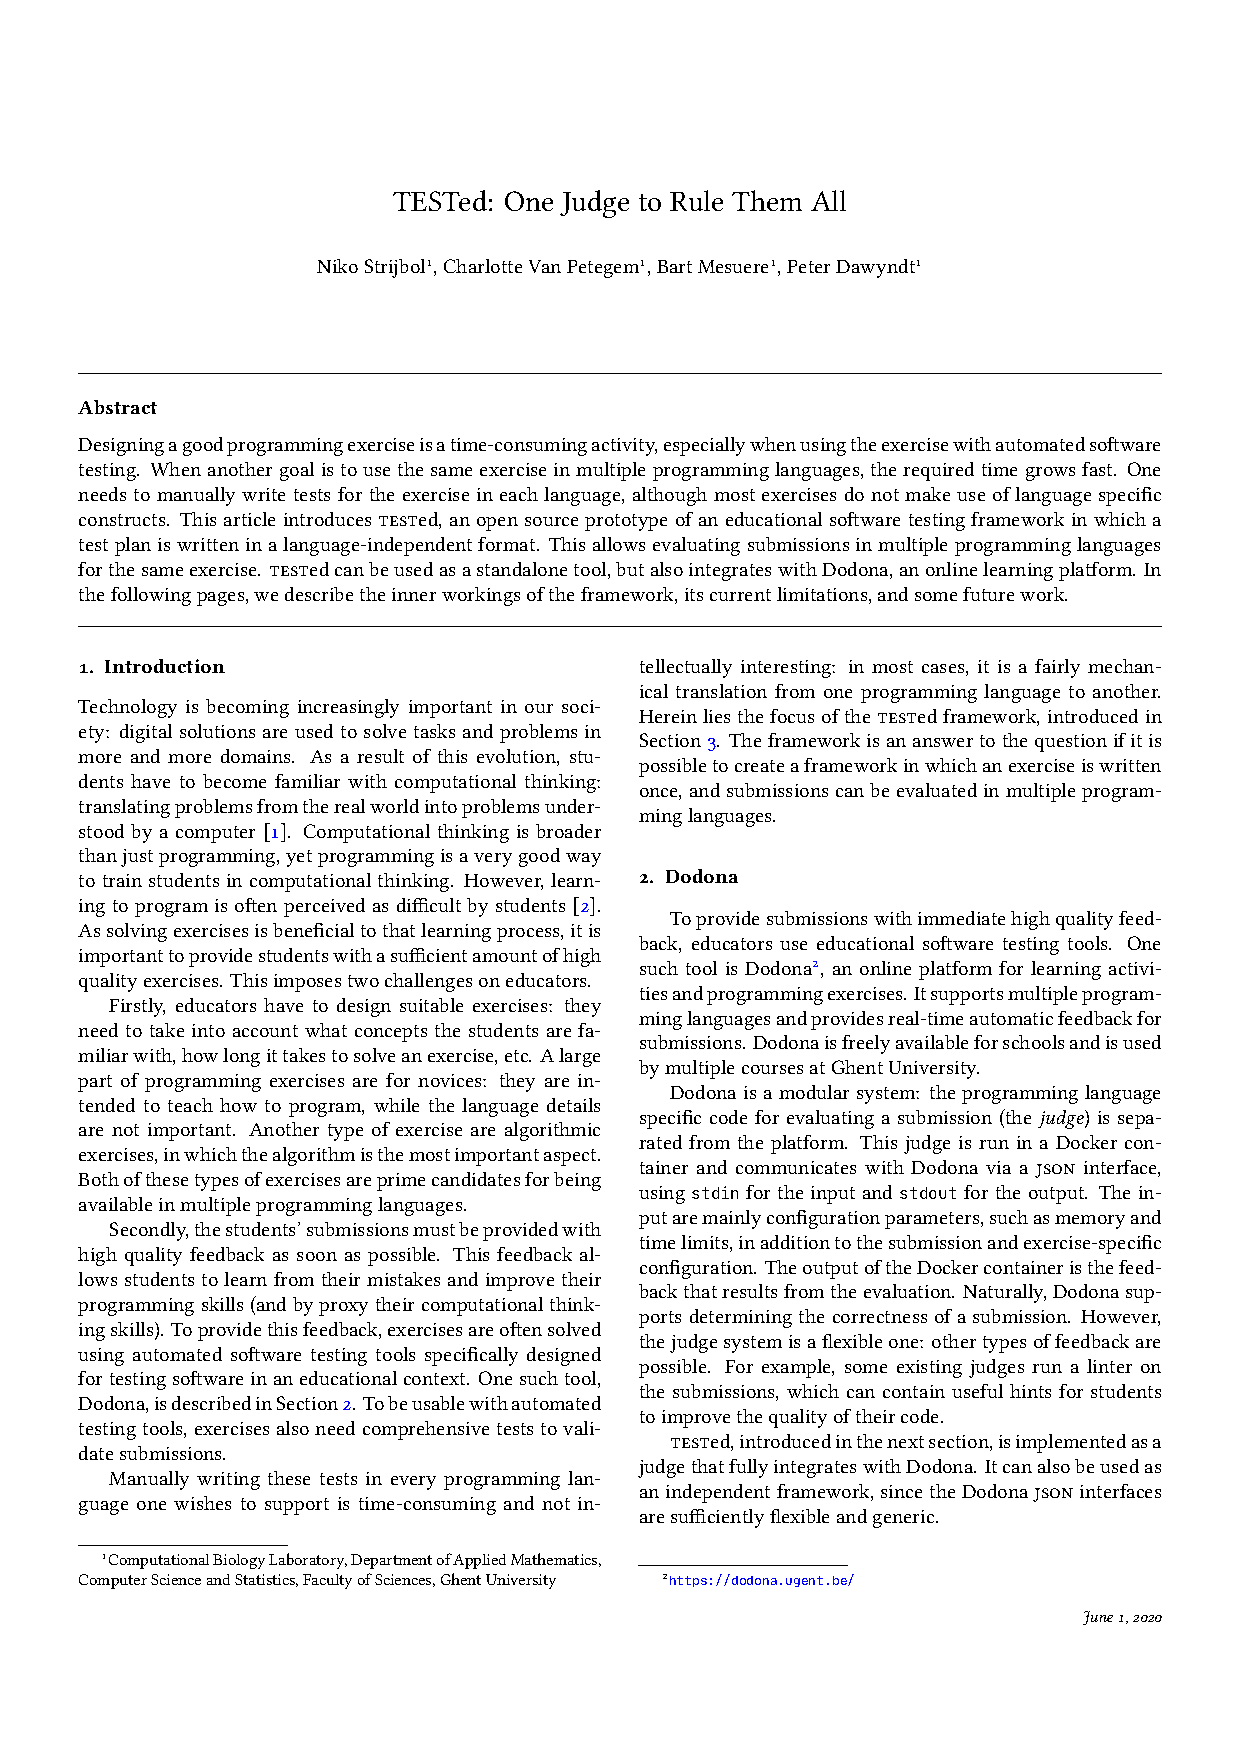
\includepdf[pages=-]{extended.pdf}
    
    \chapter*{Vulgariserende samenvatting}

In onze maatschappij wordt technologie en informatica in het bijzonder steeds belangrijker.
In steeds meer sectoren worden problemen opgelost met behulp van de computer.
Het is daarom belangrijk dat iedereen een basis digitale geletterdheid heeft.
Het is niet voldoende te kunnen werken met de programma's en technologie van vandaag.
Wie weet of programma's zoals Word of PowerPoint binnen twintig jaar nog relevant zijn?
De technologie verandert snel, waardoor het nodig is een begrip van de onderliggende systemen te hebben.

Zo komen we aan bij het begrip \emph{computationeel denken}.
Computationeel denken is een breed begrip, maar een goede invulling is het oplossen van problemen met behulp van de computer.
Het gaat om het vertalen van het probleem uit de "echte wereld" naar de informaticawereld, zodat het probleem kan begrepen worden door een computer.
Dit computationeel denken is recent ook opgenomen in de eindtermen van zowel het basisonderwijs als het secundair onderwijs.

Een goede manier om computationeel denken aan te leren aan studenten is programmeren.
Studenten ervaren programmeren echter vaak als moeilijk.
Het spreekwoord "oefening baart kunst" indachtig, denken we dat het maken van veel oefeningen een goede manier is om programmeren onder de knie te krijgen.
Het aanbieden van veel oefeningen leidt tot uitdagingen voor de lesgevers:

\begin{enumerate}
    \item Lesgevers moeten geschikte oefeningen opstellen, aangepast aan het niveau van de studenten.
    Oefeningen moeten rekening houden met welke concepten studenten al kennen, hoeveel werk het oplossen is, enzovoort.
    \item De oplossingen voor deze oefeningen moeten voorzien worden van kwalitatieve feedback.
    Enkel en alleen oefeningen oplossen is niet voldoende: goede feedback laat toe dat studenten hun vaardigheden verbeteren, doordat ze een idee krijgen wat beter kon of waar ze fout zaten.
\end{enumerate}

Voor de tweede uitdaging wordt vaak gebruikt gemaakt van een platform voor programmeeroefeningen, dat een eerste vorm van automatische feedback geeft, zoals de correctheid van de ingediende oplossing voor een oefening.
Aan de onderzoeksgroep Computationele Biologie van de UGent is hiervoor het Dodona-platform ontwikkeld.

Een ander aspect is dat er veel programmeertalen zijn en elk van die programmeertalen heeft oefeningen nodig.
Momenteel gebeurt het vertalen van een oefening van een programmeertaal naar de andere manueel.
Dit neemt ook veel tijd in beslag, terwijl veel oefeningen niet programmeertaalafhankelijk zijn.
Veel programmeeroefeningen zijn eenvoudig en komen neer op een lijst sorteren, woorden zoeken in een bestand, iets berekenen op basis van gegevens enzovoort.
Deze dingen kunnen in elke programmeertaal.

In deze thesis zoeken we naar een oplossing voor dit laatste probleem: is het mogelijk om de oefeningen één keer op een programmeertaalonafhankelijke manier te schrijven en toch oplossingen in verschillende programmeertalen te aanvaarden?

Als onderdeel van het antwoord op deze vraag hebben we een prototype van een nieuwe judge voor het Dodona-platform ontwikkeld (een judge in Dodona is het onderdeel dat verantwoordelijk is voor het beoordelen van een ingediende oplossing): \tested{}.
In \tested{} moet de lesgever voor een oefening een programmeertaalonafhankelijk testplan opstellen.
Dit testplan bevat de specificatie van hoe een ingediende oplossing beoordeeld moet worden.
Daarna vertaalt \tested{} dit testplan naar de verschillende programmeertalen, waardoor één oefening opgelost kan worden in de programmeertalen die \tested{} momenteel ondersteunt: Python, Java, JavaScript, Haskell en C.\@

Een bijkomend voordeel van \tested{} is dat we aandacht besteed hebben aan het zo eenvoudig mogelijk houden om nieuwe programmeertalen aan \tested{} toe te voegen.
Als we een nieuwe programmeertaal toevoegen aan \tested{}, zullen bestaande oefeningen ook meteen opgelost kunnen worden in deze nieuwe programmeertaal, zonder dat er iets moet veranderen aan het testplan van die oefeningen.

    \chapter*{Dankwoord}\label{ch:dankwoord}

De masterproef als culminatie van de opleiding maakt het mijn aangename plicht om ieder te bedanken met wie ik in contact ben gekomen tijdens deze opleiding, in het bijzonder de professoren, assistenten en ondersteunend personeel, die deze opleiding mogelijk gemaakt hebben.
Daarnaast zijn er enkele personen wier steun een expliciete vermelding verdient.

In de eerste plaats wil ik mijn promotoren, prof.\ dr.\ Peter Dawyndt en dr.\ Bart Mesuere, en mijn begeleiding, Charlotte Van Petegem, bedanken.
Niet alleen voor het aanbieden van dit onderwerp, waarzonder deze masterproef niet zou bestaan, maar ook voor al hun tijd en moeite die ze in deze masterproef gestoken hebben.
Zonder de wekelijkse thesismeetings, het nalezen van de verschillende iteraties van de tekst en de vele suggesties zou de masterproef niet zijn wat ze nu is.
Ik wil ook prof.\ Dawyndt in het bijzonder bedanken voor het grondig nalezen van de tekst en het uitproberen van wat ik geschreven heb.

Verder wil ik de leden van Zeus \acronym{WPI} bedanken, die ervoor zorgden dat er in de kelder altijd wel iets anders te doen was dan werken aan de masterproef.
Het is jammer dat ik hen in het tweede semester heb moeten missen.

Tot slot wil ik mijn familie bedanken voor hun onvoorwaardelijke steun en gezelschap, waardoor het ook thuis aangenaam werken was.

\begin{flushright}
    Niko Strijbol
\end{flushright}

    \chapter*{Toelating tot bruikleen}

De auteur geeft de toelating deze masterproef voor consultatie beschikbaar te stellen en delen van de masterproef te kopiëren voor persoonlijk gebruik.
Elk ander gebruik valt onder de bepalingen van het auteursrecht, in het bijzonder met betrekking tot de verplichting de bron uitdrukkelijk te vermelden bij het aanhalen van resultaten uit deze masterproef.

\shortstack{Niko Strijbol \\ \today}


    \addtocounter{tocdepth}{-1}
    \tableofcontents

    \newpage
    
    \pagenumbering{arabic}

    \chapter{Educational software testing}\label{ch:dodona}

\lettrine{D}{e evoluties} op technologisch vlak hebben ervoor gezorgd dat onze maatschappij de laatste decennia in hoge mate gedigitaliseerd is, een proces dat nog steeds aan de gang is.
Bovendien kan, door de snelheid waarmee deze veranderingen vaak optreden, eerder gesproken worden van een revolutie dan een evolutie: de veranderingen zijn vaak ingrijpend en veranderen fundamentele aspecten van de sectoren waarin de digitalisering plaatsvindt.
Dit gaat over nieuwe sectoren, zoals de deeleconomie, of ingrijpende veranderingen bij bestaande sectoren, zoals de opkomst van \english{ride sharing} in de taxisector.
Ook de impact op maatschappelijk vlak, zoals de sociale media in de politiek, mag niet vergeten worden \autocite{hipeac2019}.

Ook op educatief vlak heeft de digitalisering een grote impact.
Enerzijds biedt digitalisering nieuwe mogelijkheden aan voor onderwijsdoeleinden, zoals het lesgeven op afstand, het online aanbieden van leermateriaal en het online indienen en verbeteren van opdrachten.

Anderzijds biedt het ook uitdagingen: om studenten voor te bereiden op de steeds digitalere maatschappij is een basis van digitale geletterdheid nodig.
Net door de snelle evolutie op technologisch vlak volstaat het niet om studenten te leren werken met de technologie van vandaag;
een grondige kennis van de onderliggende werking van de technologie is onontbeerlijk.

Een belangrijk aspect hierin is het concept van \term{computationeel denken}.
Dat het aanleren van digitale vaardigheden nodig is, bewijst ook de opname van dat computationeel denken in de eindtermen, bijvoorbeeld in het katholieke basisonderwijs \autocite{zinin2017} of in het secundair onderwijs \autocite{2019040867}.

\section{Computationeel denken}\label{sec:computationeel-denken}

Op de vraag wat computationeel denken nu precies betekent lopen de antwoorden uiteen.
Het Departement Onderwijs en Vorming van de Vlaams Overheid \autocite{bastiaensen2017} definieert de term als volgt:

\begin{displayquote}
    Computationeel denken verwijst dus naar het menselijke vermogen om complexe problemen op te lossen en daarbij computers als hulpmiddel te zien.
    Met andere woorden, computationeel denken is het proces waarbij aspecten van informaticawetenschappen herkend worden in de ons omringende wereld, en waarbij de methodes en technieken uit de informaticawetenschappen toegepast worden om problemen uit de fysische en virtuele wereld te begrijpen en op te lossen.
\end{displayquote}

Computationeel denken is dus ruimer dan programmeren, maar programmeren vormt wel een uitstekende manier om het computationeel denken aan te leren en te oefenen.
Bovendien is programmeren op zich ook een nuttige vaardigheid om studenten aan te leren.

\section{Programmeeroefeningen}\label{sec:programmeeroefeningen}

Het aanleren van programmeren is niet eenvoudig en wordt door veel studenten als moeilijk ervaren \autocite{10.1145/3293881.3295779}.
Het maken van oefeningen kan daarbij helpen, indachtig het spreekwoord "oefening baart kunst".
Studenten veel oefeningen laten maken, resulteert wel in twee uitdagingen voor de lesgevers:
\begin{enumerate}
    \item Lesgevers moeten geschikte oefeningen opstellen, die rekening houden met welke programmeerconcepten studenten al kennen, tijdslimieten, moeilijkheidsgraden, enz.
    Het opstellen van deze oefeningen vraagt veel tijd.
    \item De oplossingen voor deze oefeningen moeten voorzien worden van kwalitatieve feedback.
    Bij het aanleren van programmeren is feedback een belangrijk aspect om de programmeervaardigheden van de studenten te verbeteren \autocite{10.1145/2899415.2899422}.
\end{enumerate}

Deze thesis focust op de eerste uitdaging, al wordt ook ingespeeld op de tweede uitdaging, onder andere in \cref{sec:robuustheid}.
De uitdaging wordt beschouwd binnen de context van Dodona, een online leerplatform voor automatische feedback op ingediende oplossingen voor programmeeroefeningen.

\section{Het leerplatform Dodona}\label{sec:wat-is-dodona}

Sinds 2011 wordt aan de onderzoeksgroep Computationele Biologie van de Universiteit Gent gewerkt met programmeeroefeningen die in een online systeem ingediend en beoordeeld worden.
Oorspronkelijk werd hiervoor gebruik gemaakt van de \english{Sphere Online Judge} (SPOJ) \autocite{10.1007/978-3-540-78139-4_31}.
Op basis van ervaringen met SPOJ ontwikkelde de onderzoeksgroep een eigen leerplatform, Dodona, dat in september 2016 beschikbaar werd.
Het doel van Dodona is eenvoudig: lesgevers bijstaan om hun studenten niet alleen zo goed mogelijk te leren programmeren, maar dit ook op een zo efficiënt mogelijke manier te doen.

Het online leerplatform Dodona kan opgedeeld worden in verschillende onderdelen:
\begin{enumerate}
    \item Het \textbf{leerplatform} zelf is een webapplicatie, die verantwoordelijk is om alle modules samen te laten werken en die ook de webinterface aanbiedt die de studenten en lesgevers gebruiken.
    Het is via deze interface dat lesgevers oefeningen beschikbaar maken en dat studenten hun oplossingen indienen.
    Het platform zelf is programmeertaalonafhankelijk geschreven.
    \item De \textbf{judges} binnen Dodona zijn verantwoordelijk voor het beoordelen van ingediende oplossingen.
    Dit onderdeel wordt uitgebreid besproken in \cref{sec:evalueren-van-een-oplossing}.
    \item De \textbf{oefeningen} worden niet in Dodona zelf aangemaakt, maar worden door de lesgever aangeleverd via een git-repository.
    De oefeningen bevatten de beschrijving van de opgave en de testen die uitgevoerd worden tijdens het automatisch beoordelen van een oplossing.
\end{enumerate}

Met Dodona kunnen lesgevers een leertraject opstellen door een reeks oefeningen te selecteren.
Studenten die dit leertraject volgen, zien onmiddellijk hun voortgang binnen het traject.
Bij het indienen van hun oplossingen ontvangen de studenten ook onmiddellijk feedback over hun oplossing: deze feedback bevat niet alleen de correctheid van de oplossing, maar kan ook andere aspecten belichten, zoals de kwaliteit (bv.\ de programmeerstijl), het resultaat van het uitvoeren van linters, en de performantie van de oplossing.

\section{Beoordelen van oplossingen}\label{sec:evalueren-van-een-oplossing}

In Dodona wordt elke ingediende oplossing beoordeeld door een evaluatieprogramma, de \termen{judge}.
In wezen is dit een eenvoudig programma: via de standaardinvoerstroom (\texttt{stdin}) krijgt het programma een configuratie binnen van Dodona.
Deze configuratie bevat onder andere de programmeertaal van de ingediende oplossing, de locatie van de oefeningenbestanden (die opgesteld zijn door de lesgever), de locatie van de ingediende oplossing zelf en configuratieopties, zoals geheugen- en tijdslimieten.
Het resultaat van de beoordeling wordt uitgeschreven naar de standaarduitvoerstroom (\texttt{stdout}).
Zowel de invoer als de uitvoer van de judge zijn JSON, waarvan het formaat vastgelegd is in JSON Schema.\footnote{Dit schema en een tekstuele beschrijving ervan is te vinden in de handleiding op \url{https://dodona-edu.github.io/en/guides/creating-a-judge/}.}

Concreet wordt elke beoordeling uitgevoerd in een Docker-container.
Deze Docker-container wordt gemaakt op basis van een Docker-image die bij de judge hoort, en alle dependencies bevat die de judge in kwestie nodig heeft.
Bij het uitvoeren van de beoordeling zal Dodona een \english{bind mount}\footnote{Informatie over deze term is te vinden op \url{https://docs.docker.com/storage/bind-mounts/}} voorzien, zodat de code van de judge zelf, de code van de oefening en de code van de ingediende oplossing beschikbaar zijn in de container.
Via de configuratie geeft Dodona aan de judge aan waar deze bestanden zich bevinden.

Samenvattend bestaat interface tussen de judge en Dodona uit drie onderdelen:

\begin{enumerate}
    \item De judge zal uitgevoerd worden in een Docker-container, dus een Docker-image met alle dependencies moet voorzien worden.
    Deze Docker-image moet ook de judge opstarten.
    \item De judge stelt de invoer van een beoordeling ter beschikking voor de judge.
    Bestanden worden via een bind mount aan de Docker-container gekoppeld.
    De paden naar deze bestanden binnen de container en andere informatie (zoals programmeertaal van de oplossing of natuurlijke taal van de gebruiker) worden via de configuratie aan de judge gegeven (via de standaardinvoerstroom).
    \item De judge moet het resultaat van zijn beoordeling uitschrijven naar de standaarduitvoerstroom, in een vastgelegd formaat.
\end{enumerate}

Buiten deze interface legt Dodona geen vereisten op aan de werking van judge.
Door deze vrijheid lopen de manieren waarop de bestaande judges geïmplementeerd zijn uiteen.
Sommige judges beoordelen oplossingen in dezelfde programmeertaal als de taal waarin ze geschreven zijn.
Zo is de judge voor Python-oplossingen geschreven in Python en de judge voor Java-oplossingen in Java.
Bij andere judges is dat niet het geval: de judges voor Bash en Prolog zijn bijvoorbeeld ook in Python geschreven.
Daarnaast heeft elke judge een eigen manier waarop de testen voor een beoordeling van een oplossing opgesteld moeten worden.
Zo worden in de Java-judge jUnit-testen gebruikt, terwijl de Python-judge doctests (en een eigen formaat) ondersteunt.

De beoordeling van een oplossing van een student verloopt als volgt:

\begin{enumerate}
    \item De student dient de oplossing in via de webinterface van Dodona.
    \item Dodona start een Docker-container voor de judge.
    \item Dodona voorziet de container van de bestanden van de judge, de oefening en de ingediende oplossing.
    \item De judge wordt uitgevoerd met de configuratie als op de standaardinvoerstroom.
    \item De judge beoordeelt de oplossing aan de beoordelingsmethodes opgesteld door de lesgever (d.w.z.\ de jUnit-test, de doctests, \ldots).
    Judges kunnen ook bijkomende taken uitvoeren, zoals linting, beoordeling van de performantie of \english{grading} van de code van de oplossing.
    \item De judge vertaalt zijn beoordeling naar het Dodona-formaat en schrijft het resultaat naar de standaarduitvoerstroom.
    \item Dodona slaat dat resultaat op in de databank.
    \item Op de webinterface krijgt de student het resultaat te zien als feedback op de ingediende oplossing.
\end{enumerate}

\section{Probleemstelling}\label{sec:probleemstelling}

De manier waarop de huidige judges werken resulteert in twee belangrijke nadelen.
Bij het bespreken hiervan is het nuttig een voorbeeld in het achterhoofd te houden, teneinde de nadelen te kunnen concretiseren.
Als voorbeeld gebruiken we de "Lotto"-oefening\footnote{Vrij naar een oefening van prof.\ Dawyndt.
De originele oefening is beschikbaar op \url{https://dodona.ugent.be/nl/exercises/2025591548/}}, waarvan de opgave gegeven is in \cref{lst:lotto}.
Oplossingen voor deze oefening staan in \cref{lst:java-solution,lst:python-solution}, voor respectievelijk Python en Java.

\begin{listing}
    \begin{quote}
        \markdownInput{generated/description.md}
    \end{quote}
    \caption{De opgave van de voorbeeldoefening, Lotto.}
    \label{lst:lotto}
\end{listing}

\begin{listing}
    \inputminted{python3}{../../exercise/lotto/solution/correct.py}
    \caption{Oplossing in Python voor de voorbeeldoefening Lotto.}
    \label{lst:python-solution}
\end{listing}

\begin{listing}
    \inputminted{java}{../../exercise/lotto/solution/correct.java}
    \caption{Oplossing in Java voor de voorbeeldoefening Lotto.}
    \label{lst:java-solution}
\end{listing}

\subsection*{Opstellen van oefeningen}\label{subsec:opstellen-van-oefeningen}

Het eerste en belangrijkste nadeel aan de werking van de huidige judges heeft betrekking op de lesgevers en komt voor als zij een oefening willen aanbieden in meerdere programmeertalen.
Enerzijds is dit een zware werklast: de oefening, en vooral de code voor de beoordeling, moet voor elke judge opnieuw geschreven worden.
Voor de Python-judge zullen doctests nodig zijn, terwijl de Java-judge jUnit-testen vereist.
Anderzijds lijdt dit ook tot verschillende versies van dezelfde oefening, wat het onderhouden van de oefeningen moelijker maakt.
Als er bijvoorbeeld een fout sluipt in de beoordelingscode, zal de lesgever er aan moeten denken om de fout te verhelpen in alle varianten van de oefening.
Bovendien geeft elke nieuwe versie van de oefening een nieuwe mogelijkheid voor het introduceren van fouten.

Kijkt men naar de Lotto-oefening, dan valt op dat het gaat om een eenvoudige opgave en een eenvoudige oplossing.
Bovendien zijn de verschillen tussen oplossingen in verschillende programmeertalen niet zo groot.
In de voorbeeldoplossingen in Python en Java zijn de verschillen minimaal, zij het dat de Java-oplossing wat langer is.
De Lotto-oefening zou zonder problemen in nog vele andere programmeertalen opgelost kunnen worden.
Eenvoudige programmeeroefeningen, zoals de Lotto-oefening, zijn voornamelijk nuttig in twee gevallen: studenten die voor het eerst leren programmeren en studenten die een nieuwe programmeertaal leren.
In het eerste geval is de eigenlijke programmeertaal minder relevant: het zijn vooral de concepten die belangrijk zijn.
In het tweede geval is de programmeertaal wel van belang, maar moeten soortgelijke oefeningen gemaakt worden voor elke programmeertaal die aangeleerd moet worden.
In beide gevallen is het dus een meerwaarde om de oefening in meerdere programmeertalen aan te bieden.

Eenzelfde constatatie kan gemaakt worden bij meer complexe oefeningen die zich concentreren op algoritmen: ook daar zijn de concepten belangrijker dan in welke programmeertaal een algoritme uiteindelijk geïmplementeerd wordt.
Een voorbeeld hiervan is het vak "Algoritmen en Datastructuren", dat gegeven wordt door prof.\ Fack binnen de opleiding wiskunde\footnote{De studiefiche is beschikbaar op \url{https://studiegids.ugent.be/2019/NL/studiefiches/C002794.pdf}}.
Daar zijn de meeste opgaven op Dodona vandaag al beschikbaar in de programmeertalen Java en Python, maar dan als afzonderlijke en onafhankelijke oefeningen.

Een ander aspect is de beoordeling van een oefening.
Voor de Lotto-oefening is de beoordeling niet triviaal, door het gebruik van niet-deterministische functies.
Het volstaat voor dit soort oefeningen niet om de uitvoer geproduceerd door de oplossing te vergelijken met een op voorhand vastgelegde verwachte uitvoer.
De geproduceerde uitvoer zal moeten gecontroleerd worden met code, specifiek gericht op deze oefening, die de verwachte vereisten van de oplossing controleert.
Deze evaluatiecode moet momenteel voor elke programmeertaal en dus elke judge opnieuw geschreven worden.
In de context van de Lotto-oefening controleert deze code bijvoorbeeld of de gegeven getallen binnen het bereik liggen en of ze gesorteerd zijn.
Toch is deze evaluatiecode niet inherent programmeertaalafhankelijk: controleren of een lijst gesorteerd is, heeft weinig te maken met de programmeertaal van de oplossing.

\subsection*{Implementeren van judges}\label{subsec:implementeren-van-judges}

Een tweede nadeel aan de huidige werking zijn de judges zelf: voor elke programmeertaal die men wil aanbieden in Dodona moet een nieuwe judge ontwikkeld worden.
Ook hier is er dubbel werk: dezelfde concepten en features, die eigenlijk programmeertaalonafhankelijk zijn, moeten in elke judge opnieuw geïmplementeerd worden.
Hierbij denken we aan bijvoorbeeld de logica om te bepalen wanneer een beoordeling positief of negatief moet zijn.

\subsection*{Onderzoeksvraag}\label{subsec:onderzoeksvraag}

Het eerste nadeel wordt beschouwd als het belangrijkste nadeel en de focus van deze thesis.
Het nadeel valt te formuleren als de onderzoeksvraag waarop deze thesis een antwoord wil bieden:

\begin{quote}
    Is het mogelijk om een judge zo te implementeren dat de opgave en beoordelingsmethoden van een oefening slechts eenmaal opgesteld dienen te worden, waarna de oefening beschikbaar is in alle programmeertalen die de judge ondersteunt?
    Hierbij is het wenselijk dat eens een oefening opgesteld is, deze niet meer gewijzigd moet worden wanneer talen toegevoegd worden aan de judge.
\end{quote}

Als bijzaak is het ook interessant om na te gaan of het antwoord op de onderzoeksvraag een voordeel kan bieden voor het implementeren van judges zelf.

De aandachtige lezer zal opmerken dat de opgave voor de Lotto-oefening (\cref{lst:lotto}) programmeertaalspecifieke en taalspecifieke elementen bevat.
Zo zijn de voorbeelden in Python en zijn de namen van functies en argumenten in het Nederlands.
Het ondersteunen van opgaves met programmeertaalonafhankelijke voorbeelden en vertalingen wordt voor deze thesis expliciet als \english{out-of-scope} gezien en zal niet behandeld worden, zij het in \cref{subsec:programmeertaalonafhankelijke-opgaven}.

\section{Opbouw van de thesis}\label{sec:opbouw}

\Cref{ch:de-universele-judge} handelt over het antwoord op bovenstaande onderzoeksvraag, waar een prototype van een dergelijke judge wordt voorgesteld.
Daarna volgt ter illustratie een gedetailleerde beschrijving van hoe een oefening opgesteld moet worden voor dit prototype.
Nadien volgt een beschrijving van hoe een nieuwe programmeertaal moet toegevoegd worden aan het prototype.
Daar deze twee hoofdstukken voornamelijk ten doel hebben zij die met het prototype (zoals lesgevers) moeten werken te informeren, nemen deze hoofdstukken de vorm aan van meer traditionele softwarehandleidingen.
Tot slot volgt met een hoofdstuk over beperkingen van de huidig prototype, en waar er verbeteringen mogelijk zijn (het "toekomstige werk").

    \chapter{TESTed}\label{ch:de-universele-judge}

\lettrine{I}{n het kader} van deze masterproef werd een prototype geïmplementeerd van een judge voor Dodona.
Het doel hiervan is een antwoord te bieden aan de onderzoeksvraag uit het vorige hoofdstuk en de beperkingen van deze aanpak in kaart te brengen.
Deze judge heeft de naam \term{TESTed} gekregen.
Bij TESTed is een oefening programmeertaalonafhankelijk en kunnen oplossingen in verschillende programmeertalen beoordeeld worden aan de hand van een en dezelfde specificatie.
Dit hoofdstuk begint met het ontwerp en de algemene werking van de judge toe te lichten, waarna elk onderdeel in meer detail besproken wordt.

\section{Overzicht}\label{sec:ontwerp}

\subsection{Architecturaal ontwerp}\label{subsec:architecturaal-overzicht}

\Cref{fig:universal-judge} toont het architecturaal ontwerp van TESTed.
De twee stippellijnen geven programmeertaalbarrières aan, en verdelen TESTed in drie logisch omgevingen:

\begin{enumerate}
    \item TESTed zelf is geschreven in Python: in het middelste deel staat de programmeertaal dus vast.
    Dit onderdeel is verantwoordelijk voor de regie van de beoordeling op basis van het testplan.
    \item De ingediende oplossing wordt uitgevoerd in de \term{uitvoeringsomgeving}, waar de programmeertaal overeenkomt met de programmeertaal van de oplossing.
    \item Tot slot is er nog de \term{evaluatieomgeving}, waar door de lesgever geschreven evaluatiecode wordt uitgevoerd.
    Deze moet niet in dezelfde programmeertaal als de oplossing of TESTed geschreven zijn.
\end{enumerate}

\subsection{Stappenplan van een beoordeling}\label{subsec:stappenplan-van-een-beoordeling}

De rest van het hoofdstuk bespreekt alle onderdelen van en stappen die gebeuren bij een beoordeling van een ingediende oplossing in detail.
In \cref{fig:tested-flow} zijn deze stappen gegeven als een flowchart, en een uitgeschreven versie volgt:

\begin{enumerate}
    \item De Docker-container voor TESTed wordt gestart.
    Dodona stelt de invoer ter beschikking aan de container: het testplan komt uit de oefening, terwijl de ingediende oplossing en de configuratie uit Dodona komen.
    \item Als eerste stap wordt gecontroleerd dat het testplan de programmeertaal van de ingediende oplossing ondersteunt.
    De programmeertaal van de oplossing wordt gegeven via de configuratie uit Dodona.
    Merk op dat de ingediende oplossing zelf hierbij niet nodig is: deze controle zou idealiter gebeuren bij het importeren van de oefening in Dodona, zodat Dodona weet in welke programmeertalen een bepaalde oefening aangeboden kan worden (zie \cref{ch:beperkingen-en-toekomstig-werk}).
    Als het testplan bijvoorbeeld programmeertaalspecifieke code bevat die enkel in Java geschreven is, zal een oplossing in Python niet beoordeeld kunnen worden.
    Bevat het testplan bijvoorbeeld een functie die een verzameling moet teruggeven, dan zullen talen als Bash niet in aanmerking komen.
    \item Het testplan (details in \cref{subsec:het-testplan}) bestaat uit verschillende contexten.
    Elke context is een onafhankelijke uitvoering van de ingediende oplossing en kan verschillende aspecten van die uitvoering beoordelen.
    Voor elk van die contexten wordt in deze stap de testcode gegenereerd.
    Deze stap is de overgang naar de \term{uitvoeringsomgeving}.
    \item De testcode wordt optioneel gecompileerd.
    Dit kan op twee manieren gebeuren (details in \cref{subsec:testcode-genereren}):
    \begin{enumerate}
        \item Batchcompilatie: hierbij wordt de testcode van alle contexten verzameld en gecompileerd tot één uitvoerbaar bestand (executable).
        Dit heeft als voordeel dat er slechts een keer een compilatie nodig is, wat voor een betere performantie zorgt.
        Bij deze manier resulteert de compilatiestap in één uitvoerbaar bestand.
        \item Contextcompilatie: hierbij wordt de testcode voor elke context afzonderlijk gecompileerd tot een uitvoerbaar bestand.
        Bij deze manier worden er $n$ uitvoerbare bestanden geproduceerd tijdens de compilatiestap.
    \end{enumerate}
    In talen die geen compilatie nodig hebben of ondersteunen, wordt deze stap overgeslagen.
    \item Nu kan het uitvoeren van de beoordeling zelf beginnen: de gegenereerde code wordt uitgevoerd (nog steeds in de uitvoeringsomgeving).
    Elke context uit het testplan wordt in een afzonderlijk subproces uitgevoerd, teneinde het delen van informatie tegen te gaan.
    De onafhankelijkheid van de contexten laat ons ook toe om contexten in parallel uit te voeren.
    \item De uitvoering van de executable in de vorige stap produceert resultaten (voor elke context), zoals de standaarduitvoerstroom, de standaardfoutstroom, returnwaardes, exceptions of exitcodes.
    Deze bundel resultaten wordt nu geëvalueerd op juistheid.
    Hiervoor zijn drie mogelijke manieren:
    \begin{enumerate}
        \item Programmeertaalspecifieke evaluatie (afgekort tot SE in de flowchart).
        De code voor de evaluatie is opgenomen in de executable en wordt onmiddellijk uitgevoerd in hetzelfde proces.
        Via deze mogelijkheid kunnen taalspecifieke aspecten gecontroleerd worden.
        Daar de evaluatie in hetzelfde proces gebeurt, blijft dit in de uitvoeringsomgeving.
        \item Geprogrammeerde evaluatie (afgekort tot PE in de flowchart).
        Hierbij is er evaluatiecode geschreven die los staat van de oplossing, waardoor deze evaluatiecode ook in een andere programmeertaal geschreven kan zijn.
        De code ter uitvoering van de geprogrammeerde evaluatiecode wordt gegenereerd en dan uitgevoerd.
        Het doel van deze modus is om complexe evaluaties toe te laten op een programmeertaalonafhankelijke manier.
        Deze stap vindt plaats in de evaluatieomgeving.
        \item Generieke evaluatie.
        Hierbij evalueert TESTed zelf het resultaat.
        Deze modus is bedoeld voor gestandaardiseerde evaluaties, zoals het vergelijken van geproduceerde uitvoer en verwachte uitvoer.
        Hier gebeurt de evaluatie binnen TESTed zelf.
    \end{enumerate}
    \item Tot slot verzamelt TESTed alle evaluatieresultaten en stuurt ze gebundeld door naar Dodona, waarna ze getoond worden aan de gebruiker.
\end{enumerate}

\begin{figure}
    \centering
    \documentclass[class=ugent2016-report,crop=false]{standalone}

\usepackage{tikz}
\usetikzlibrary{shapes,arrows,positioning,backgrounds,calc,intersections,calc}
\usepackage[top=2cm, bottom=2cm, left=2cm, right=2cm]{geometry}

\begin{document}


    % Define the styles for various components in the architectural diagram.
    \tikzstyle{node}=[draw, minimum height=1cm, text width=3cm, align=center, fill=white]
    \tikzstyle{state}=[node, rectangle]
    \tikzstyle{process}=[node, rectangle, rounded corners=0.5cm]
    \tikzstyle{named}=[text=ugent-blue,font=\sffamily\scshape,align=center,text width=3cm]

    \begin{tikzpicture}

        %\draw[step=1.0,gray,thin] (0,0) grid (15,-25);

        \node[state] (input) at (7.5,2) {Invoer};

        \node[process] (generation) at (7.5,0) {Genereren \\ testcode};

        \node[state] (code) at (13.5,0) {Testcode};
        \node[process] (execution) at (13.5,-2) {Uitvoeren};

        \node[state] (execution state) at (13.5,-4) {Uitvoer};
        \node[state] (core state) at (7.5,-4) {Uitvoer};
        \node[state] (evaluation state) at (1.5,-4) {Uitvoer};

        \node[process] (custom evaluation) at (1.5,-6) {Evaluatie};
        \node[process] (core evaluation) at (7.5,-6) {Evaluatie};
        \node[process] (execution evaluation) at (13.5,-6)  {Evaluatie};

        \node[state] (feedback) at (7.5,-8) {Beoordeling};

        \node[named] (core name) at (7.5,-10) {TESTed};
        \node[named] (evaluation name) at (1.5,-10) {evaluatieomgeving};
        \node[named] (execution name) at (13.5,-10) {uitvoeringsomgeving};

        \begin{scope}[on background layer]

            % Draw these first to ensure they are in the background.
            \path[draw,dashed,very thick,lightgray] (4.5,3) -- (4.5,-11);
            \path[draw,dashed,very thick,lightgray] (10.5,3) -- (10.5,-11);

            \draw [->] (input) -- (generation);
            \draw[->] (generation) -- (code);
            \draw[->] (code) -- (execution);
            \draw[->] (execution) -- (execution state);
            \draw[->] (execution state) -- node[above] {Serialisatie} ++ (core state);
            \draw[->] (core state) -- node[above] {Deserialisatie} ++ (evaluation state);
            \draw[->] (core state) -- (core evaluation);
            \draw[->] (evaluation state) -- (custom evaluation);
            \draw[->] (execution state) -- (execution evaluation);

            \draw[->] (core evaluation.south) -- (feedback);
            \draw[->] (custom evaluation.south) -- (feedback.west);
            \draw[->] (execution evaluation.south) -- (feedback.east);

        \end{scope}


    \end{tikzpicture}

\end{document}

    \caption{Schematische voorstelling van het architecturale ontwerp van de TESTed.}
    \label{fig:universal-judge}
\end{figure}

\begin{figure}
    \centering
    %! Suppress = MultipleIncludes
\documentclass[class=ugent2016-report,crop=false,12pt]{standalone}

\usepackage{tikz}
\usetikzlibrary{shapes,arrows,positioning,backgrounds,calc,intersections,calc}
\usepackage[top=2cm, bottom=2cm, left=2cm, right=2cm]{geometry}

\begin{document}

    \tikzstyle{node}=[draw, minimum height=1cm, align=center, fill=white, text height=1.5ex, text depth=.25ex]
    \tikzstyle{process}=[node, rectangle]
    \tikzstyle{terminator}=[node, rectangle, rounded corners=0.5cm]
    \tikzstyle{document}=[node,tape,tape bend top=none]
    \tikzstyle{io}=[node,trapezium,trapezium left angle=70,trapezium right angle=-70,minimum width=3cm]
    \tikzstyle{nothing}=[align=center]
    \tikzstyle{inner}=[process,draw=gray]
    \tikzstyle{arrow}=[draw, -latex]
    \tikzstyle{ind}=[fill=ugent-we!50!white]
    \tikzstyle{pre}=[fill=ugent-ps!50!white]
    \tikzstyle{inda}=[draw=ugent-we!70!black]
    \tikzstyle{prea}=[draw=ugent-ps!70!black]
    \tikzstyle{ae}=[fill=ugent-re!50!white]
    \tikzstyle{ie}=[fill=ugent-ea!50!white]
    \tikzstyle{se}=[fill=ugent-ge!50!white]
    \tikzstyle{aea}=[draw=ugent-re!70!black]
    \tikzstyle{iea}=[draw=ugent-ea!70!black]
    \tikzstyle{sea}=[draw=ugent-ge!70!black]

    \begin{tikzpicture}
%        \draw[step=1.0,gray,thin] (0,0) grid (15,-25);

        \node[io] at (5.625,-1) (exercise) {Oefening};
        \node[io] at (12.125,-1) (dodonaIn) {Dodona};
        
        % These needs to be drawn first, otherwise they are on top of the
        % input node.
        \node[process,minimum width=3cm] at (1.5,-7) (g1) {Genereren};
        \node[process,minimum width=3cm] at (5.5,-7) (g2) {Genereren};
        \node[process,minimum width=3cm] at (9.5,-7) (gn) {Genereren};

        \node[document,minimum width=3cm,text height=9ex,text depth=2ex,pre] at (13.5,-8) (ta) {Testcode 1\\Testcode 2\\Testcode $n$};

        \node[document,minimum width=3cm] at (1.5,-8.5) (t1) {Testcode 1};
        \draw[arrow,prea] (t1.10) -- (t1.10-|ta.west);
        \node[document,minimum width=3cm] at (5.5,-8.5) (t2) {Testcode 2};
        \draw[arrow,prea] (t2.east) -- (t2.east-|ta.west);
        \node[document,minimum width=3cm] at (9.5,-8.5) (tn) {Testcode $n$};
        \draw[arrow,prea] (tn.350) -- (tn.350-|ta.west);

        \node[process,minimum width=3cm,ind] at (1.5,-10) (co1) {Compileren};
        \draw[arrow] (11.5,-9.66) -- (11.5,-9.66-|co1.east);
        \node[process,minimum width=3cm,ind] at (5.5,-10) (co2) {Compileren};
        \draw[arrow] (11.5,-10) -- (11.5,-10-|co2.east);
        \node[process,minimum width=3cm,ind] at (9.5,-10) (con) {Compileren};
        \node[process,minimum width=3cm,pre] at (13.5,-10) (coa) {Compileren};

        \draw[arrow] (0,-5-|g1.120) -- (g1.120);
        \draw[arrow] (0,-5-|g2.60) -- (g2.60);
        \draw[arrow] (0,-5-|gn.60) -- (gn.60);

        % Input
        \node[document, minimum width=14cm, minimum height=4cm,tape bend height=0.5cm] at (7.5, -3.75) (input) {};

        \node[nothing] at (1.5,-2.375) {Invoer};

        \node[inner,minimum width=8.75cm, minimum height=2.25cm] at (5.625,-4) (plan) {};
        \node[nothing] at (2.5,-3.375) {Testplan};
        \node[inner,minimum width=2.25cm] at (2.75,-4.375) (c1) {Context 1};
        \node[inner,minimum width=2.25cm] at (5.25,-4.375) (c2) {Context 2};
        \node[nothing,text height=1.5ex, text depth=.25ex] at (6.875,-4.375) {\ldots};
        \node[inner,minimum width=2.25cm] at (8.5,-4.375) (cn) {Context $n$};

        \draw[arrow] (exercise.south) -- (exercise|-plan.north);

        \node[inner,minimum width=3.25cm, minimum height=1.25cm, text height=4ex] at (12.125,-4.5) (solution) {Ingediende \\ oplossing};

        \draw[arrow] (dodonaIn.south east) -- (dodonaIn.south east|-solution.north east);

        \node[inner,minimum width=3.25cm] at (12.125,-3) (config) {Configuratie};

        \draw[arrow] (11.5,-10.33|-solution.south) -- (11.5,-10.33) -- (11.5,-10.33-|con.east);
        \draw[arrow] (11.5,-10.1625) -- (11.5,-10.1625-|coa.west);

        \draw[arrow] (dodonaIn.south) -- (dodonaIn|-config.north);

        \draw[arrow] (c1) |- (g1.60|-2,-6.25) -- (g1.60);
        \draw[arrow] (c2) |- (g2.120|-6.75,-6.25) -- (g2.120);
        \draw[arrow] (cn) |- (gn.120|-12.5,-6.25) -- (gn.120);

        \draw[arrow] (g1) --(t1);
        \draw[arrow] (g2) --(t2);
        \draw[arrow] (gn) --(tn);

        \draw[arrow,inda] (t1) --(co1);
        \draw[arrow,inda] (t2) --(co2);
        \draw[arrow,inda] (tn) --(con);
        \draw[arrow,prea] (ta) --(coa);

        \node[document,minimum width=3cm,ind] at (1.5,-11.5) (e1) {Executable 1};
        \node[document,minimum width=3cm,ind] at (5.5,-11.5) (e2) {Executable 2};
        \node[document,minimum width=3cm,ind] at (9.5,-11.5) (en) {Executable $n$};
        \node[document,minimum width=3cm,pre] at (13.5,-11.5) (ea) {Executable};

        \draw[arrow,inda] (co1) --(e1);
        \draw[arrow,inda] (co2) --(e2);
        \draw[arrow,inda] (con) --(en);
        \draw[arrow,prea] (coa) --(ea);

        \node[process,minimum width=3cm] at (2.5,-13.5) (u1) {Uitvoeren};
        \node[process,minimum width=3cm] at (7.5,-13.5) (u2) {Uitvoeren};
        \node[process,minimum width=3cm] at (12.5,-13.5) (un) {Uitvoeren};

        \draw[arrow,inda] (e1) |- (u1.135|-0,-12.33) -- (u1.135);
        \draw[arrow,inda] (e2) |- (u2.135|-0,-12.33) -- (u2.135);
        \draw[arrow,inda] (en) |- (un.135|-0,-12.33) -- (un.135);

        \draw[arrow,prea] (ea) |- (u1.45|-0,-12.66) -- (u1.45);
        \draw[arrow,prea] (u2.45|-0,-12.66) -- (u2.45);
        \draw[arrow,prea] (un.45|-0,-12.66) -- (un.45);

        \node[document,minimum width=3cm] at (2.5,-15) (r1) {Resultaat 1};
        \node[document,minimum width=3cm] at (7.5,-15) (r2) {Resultaat 2};
        \node[document,minimum width=3cm] at (12.5,-15) (rn) {Resultaat $n$};

        \draw[arrow] (u1) --(r1);
        \draw[arrow] (u2) --(r2);
        \draw[arrow] (un) --(rn);

        \node[process,minimum size=1cm,ae] at (1,-16.5) (ae1) {PE};
        \node[process,minimum size=1cm,ie] at (2.5,-16.5) (ie1) {GE};
        \node[process,minimum size=1cm,se] at (4,-16.5) (se1) {SE};

        \draw[arrow,aea] (r1) --(ae1);
        \draw[arrow,iea] (r1) --(ie1);
        \draw[arrow,sea] (r1) --(se1);

        \node[process,minimum size=1cm,ae] at (6,-16.5) (ae2) {PE};
        \node[process,minimum size=1cm,ie] at (7.5,-16.5) (ie2) {GE};
        \node[process,minimum size=1cm,se] at (9,-16.5) (se2) {SE};

        \draw[arrow,aea] (r2) --(ae2);
        \draw[arrow,iea] (r2) --(ie2);
        \draw[arrow,sea] (r2) --(se2);

        \node[process,minimum size=1cm,ae] at (11,-16.5) (aen) {PE};
        \node[process,minimum size=1cm,ie] at (12.5,-16.5) (ien) {GE};
        \node[process,minimum size=1cm,se] at (14,-16.5) (sen) {SE};

        \draw[arrow,aea] (rn) --(aen);
        \draw[arrow,iea] (rn) --(ien);
        \draw[arrow,sea] (rn) --(sen);

        \node[document, minimum width=14cm, minimum height=3cm,tape bend height=0.5cm] at (7.5,-19) (b) {};

        \node[inner,minimum width=3cm,text height=4ex,minimum height=1.5cm] at (2.5,-18.75) (b1) {Beoordeling \\ context 1};
        \node[inner,minimum width=3cm,text height=4ex,minimum height=1.5cm] at (7.5,-18.75) (b2) {Beoordeling \\ context 2};
        \node[inner,minimum width=3cm,text height=4ex,minimum height=1.5cm] at (12.5,-18.75) (bn) {Beoordeling \\ context $n$};

        \draw[arrow,aea] (ae1) --(b1);
        \draw[arrow,iea] (ie1) --(b1);
        \draw[arrow,sea] (se1) --(b1);
        \draw[arrow,aea] (ae2) --(b2);
        \draw[arrow,iea] (ie2) --(b2);
        \draw[arrow,sea] (se2) --(b2);
        \draw[arrow,aea] (aen) --(bn);
        \draw[arrow,iea] (ien) --(bn);
        \draw[arrow,sea] (sen) --(bn);

        \node[nothing,fill=white] at (2,-20) {Beoordeling};

        \node[io] at (7.5,-22) (dodonaOut) {Dodona};

        \draw[arrow] (b) -- node [right] {Feedback} (dodonaOut);

    \end{tikzpicture}

\end{document}

    \caption{
        Flowchart van een beoordeling door TESTed.
        In het schema worden kleuren gebruikt als er een keuze gemaakt moet worden voor een volgende stap.
        Er kan steeds slechts één mogelijkheid gekozen worden.
        De afkortingen PE, GE en SE staan respectievelijk voor geprogrammeerde evaluatie, generieke evaluatie en (programmeertaal)specifieke evaluatie.
    }
    \label{fig:tested-flow}
\end{figure}


\section{Beschrijven van een oefening}\label{sec:testplan}

De beoordeling van een ingediende oplossing van een oefening begint bij de invoer die TESTed krijgt.
Centraal in deze invoer is een \term{testplan}, een specificatie die op een programmeertaalonafhankelijke manier beschrijft hoe een oplossing voor een oefening beoordeeld moet worden.
Het vervangt de taalspecifieke testen van de bestaande judges (ie.\ de jUnit-tests of de doctests in respectievelijk Java en Python).
Het testplan \latin{sensu lato} wordt opgedeeld in verschillende onderdelen, die hierna besproken worden.

\subsection{Het testplan}\label{subsec:het-testplan}

Het testplan \latin{sensu stricto} beschrijft de structuur van de beoordeling van een ingediende oplossing voor een oefening.
Deze structuur lijkt qua opbouw sterk op de structuur van de feedback zoals gebruikt door Dodona.
Dat de structuur van de oplossing in Dodona en van het testplan op elkaar lijken, heeft als voordeel dat er geen mentale afbeelding moet gemaakt worden tussen de structuur van het testplan en dat van Dodona.
Concreet is de structuur een hiërarchie met volgende elementen:

\begin{description}
    \item[Plan] Het top-level object van het testplan.
    Dit object bevat twee belangrijke objecten: de tabbladen en de configuratie.
    Deze configuratie is de plaats om opties aan TESTed mee te geven.
    \item[Tab] Een testplan bestaat uit verschillende \termen{tab}s of tabbladen.
    Deze komen overeen met de tabbladen in de gebruikersinterface van Dodona.
    Een tabblad kan een naam hebben, die zichtbaar is voor de gebruikers.
    \item[Context] Elk tabblad bestaat uit een of meerdere \termen{context}en.
    Een context is een onafhankelijke uitvoering van een evaluatie.
    De nadruk ligt op de "onafhankelijkheid", zoals al vermeld.
    Elke context wordt in een nieuw proces en in een eigen map (directory) uitgevoerd, zodat de kans op het delen van informatie klein is.
    Hierbij willen we vooral onbedoeld delen van informatie (zoals statische variabelen of het overschrijven van bestanden) vermijden.
    De gemotiveerde student zal nog steeds informatie kunnen delen tussen de uitvoeringen, door bv.\ in een andere locatie een bestand aan te maken en later te lezen.
    \item[Testcase] Een context bestaat uit een of meerdere \termen{testcase}s of testgevallen.
    Een testgeval bestaat uit invoer en een aantal tests.
    De testgevallen kunnen onderverdeeld worden in twee soorten:
    \begin{description}
        \item[Main testcase] of hoofdtestgeval.
        Van deze soort is er maximaal één per context (geen hoofdtestgeval is ook mogelijk).
        Dit testgeval heeft als doel het uitvoeren van de main-functie (of de code zelf als het gaat om een scripttaal zoals Bash of Python).
        Als invoer voor dit testgeval kunnen enkel de standaardinvoerstroom en de programma-argumenten meegegeven worden.
        De exitcode van een uitvoering kan ook enkel in het hoofdtestgeval gecontroleerd worden.
        \item[Normal testcase] of normaal testgeval.
        Hiervan kunnen er nul of meer zijn per context.
        Deze testgevallen dienen om andere aspecten van de ingediende oplossing te testen, nadat de code van de gebruiker met success ingeladen is.
        De invoer is dan ook uitgebreider: het kan gaan om het standaardinvoerkanaal, functieoproepen en variabeletoekenningen.
        Een functieoproep of variabeletoekenning is verplicht (zonder functieoproep of toekenning aan een variabele is er geen code om te testen).
    \end{description}
    Het hoofdtestgeval wordt altijd als eerste uitgevoerd.
    Dit is verplicht omdat bepaalde programmeertalen (zoals Python en andere scripttalen) de code onmiddellijk uitvoeren bij het inladen.
    Om te vermijden dat de volgorde van de testgevallen zou verschillen tussen de programmeertalen, wordt het hoofdtestgeval altijd eerst uitgevoerd.
    \item[Test] De beoordeling van een testgeval bestaat uit meerdere \term{test}s, die elk één aspect van het testgeval controleren.
    Met aspect bedoelen we de standaarduitvoerstroom, de standaardfoutstroom, opgevangen uitzonderingen (\english{exceptions}), de teruggegeven waarden van een functieoproep (returnwaarden) of de inhoud van een bestand.
    De exitcode is ook mogelijk, maar enkel in het hoofdtestgeval.
    Het beoordelen van de verschillende aspecten wordt in meer detail beschreven in \cref{sec:oplossingen-beoordelen}
\end{description}

Bij de keuze voor een formaat voor het testplan (json, xml, \ldots), zijn vooraf enkele vereisten geformuleerd waaraan het gekozen formaat moet voldoen.
Het moet:

\begin{itemize}
    \item leesbaar zijn voor mensen,
    \item geschreven kunnen worden met minimale inspanning, met andere woorden de syntaxis dient eenvoudig te zijn, en
    \item programmeertaalonafhankelijk zijn.
\end{itemize}

Uiteindelijk is gekozen om het testplan op te stellen in json.
Niet alleen voldoet json aan de vooropgestelde voorwaarden, het wordt ook door veel talen ondersteund.

Toch zijn er ook enkele nadelen aan het gebruik van json.
Zo is json geen beknopte of compacte taal om met de hand te schrijven.
Een oplossing hiervoor gebruikt de eigenschap dat veel talen json kunnen produceren: andere programma's kunnen desgewenst het testplan in het json-formaat genereren, waardoor het niet met de hand geschreven moet worden.
Hiervoor denken we aan een \termen{DSL} (\english{domain specific language}), maar dit valt buiten de thesis en wordt verder besproken in \cref{ch:beperkingen-en-toekomstig-werk}.

Een tweede nadeel is dat json geen programmeertaal is.
Terwijl dit de implementatie van de judge bij het interpreteren van het testplan weliswaar eenvoudiger maakt, is het tevens beperkend: beslissen of een testgeval moet uitgevoerd worden op basis van het resultaat van een vorig testgeval is bijvoorbeeld niet mogelijk.
Ook deze beperking wordt uitgebreider besproken in \cref{ch:beperkingen-en-toekomstig-werk}.

Tot slot bevat \cref{lst:testplan} een testplan met één context voor de voorbeeldoefening Lotto uit \cref{ch:dodona}.

\begin{listing}
    \inputminted{python}{code/testplan.json}
    \caption{
        Een ingekorte versie van het testplan voor de voorbeeldoefening Lotto.
        Het testplan bevat maar één context.
    }
    \label{lst:testplan}
\end{listing}

\subsection{Dataserialisatie}\label{subsec:dataserialisatie}

Bij de beschrijving van het testplan wordt gewag gemaakt van returnwaarden en variabeletoekenningen.
Aangezien het testplan programmeertaalonafhankelijk is, moet er dus een manier zijn om data uit de verschillende programmeertalen voor te stellen en te vertalen: het \term{serialisatieformaat}.

\subsubsection{Keuze van het formaat}

Zoals bij het testplan, werd voor de voorstelling van waarden ook een keuze voor een bepaald formaat gemaakt.
Daarvoor werden opnieuw enkele voorwaarden vooropgesteld, waaraan het serialisatieformaat moet voldoen.
Het formaat moet:

\begin{itemize}
    \item door mensen geschreven kunnen worden (\english{human writable}),
    \item onderdeel van het testplan kunnen zijn,
    \item in meerdere programmeertalen bruikbaar zijn, en
    \item de basisgegevenstypes ondersteunen die we willen aanbieden in het programmeertaalonafhankelijke deel van het testplan.
    Deze gegevenstypes zijn:
    \begin{itemize}
        \item Primitieven: gehele getallen, reële getallen, Boolese waarden en tekenreeksen.
        \item Collecties: rijen (eindige, geordende reeks; \texttt{list} of \texttt{array}), verzamelingen (eindige, ongeordende reeks zonder herhaling; \texttt{set}) en afbeeldingen (elk element wordt afgebeeld op een ander element; \texttt{map}, \texttt{dict} of \texttt{object}).
    \end{itemize}
\end{itemize}

Een voor de hand liggende oplossing is om ook hiervoor json te gebruiken, en zelf in json een structuur op te stellen voor de waarden.
In tegenstelling tot de situatie bij het testplan bestaan er al een resem aan dataserialisatieformaten, waardoor het de moeite loont om na te gaan of er geen bestaand formaat voldoet aan de vereisten.
Hiervoor is gestart van een overzicht op Wikipedia \autocite{wiki2020}.
Uiteindelijk is niet gekozen voor een bestaand formaat, maar voor de json-oplossing.
De redenen hiervoor zijn samen te vatten als:

\begin{itemize}
    \item Het gaat om een binair formaat.
    Binaire formaten zijn uitgesloten op basis van de eerste twee voorwaarden die we opgesteld hebben: mensen kunnen het niet schrijven zonder hulp van bijkomende tools en het is moeilijk in te bedden in een json-bestand (zonder gebruik te maken van encoderingen zoals base64).
    Bovendien zijn binaire formaten moeilijker te implementeren in sommige talen.
    \item Het formaat ondersteunt niet alle gewenste types.
    Sommige formaten hebben ondersteuning voor complexere datatypes, maar niet voor alle complexere datatypes die wij nodig hebben.
    Uiteraard kunnen de eigen types samengesteld worden uit basistypes, maar dan biedt de ondersteuning voor de complexere types weinig voordeel, aangezien er toch een eigen dataschema voor die complexere types opgesteld zal moeten worden.
    \item Sommige formaten zijn omslachtig in gebruik.
    Vaak ondersteunen dit soort formaten meer dan wat wij nodig hebben.
    \item Het formaat is niet eenvoudig te implementeren in een programmeertaal waarvoor geen ondersteuning is.
    Sommige dezer formaten ondersteunen weliswaar veel talen, maar we willen niet dat het serialisatieformaat een beperkende factor wordt in welke talen door de judge ondersteund worden.
    Het mag niet de bedoeling zijn dat het implementeren van het serialisatieformaat het meeste tijd in beslag neemt.
\end{itemize}

Een lijst van de overwogen formaten met een korte beschrijving:

\begin{description}
    \item[Apache Avro] Een volledig "systeem voor dataserialisatie".
    De specificatie van het formaat gebeurt in json (vergelijkbaar met JSON Schema), terwijl de eigenlijke data binair geëncodeerd wordt.
    Heeft uitbreidbare types, met veel ingebouwde types \autocite{avro}.
    \item[Apache Parquet] Minder relevant, dit is een bestandsformaat voor Hadoop \autocite{parquet}.
    \item[ASN.1] Staat voor \english{Abstract Syntax Notation One}, een formaat uit de telecommunicatie.
    De hoofdstandaard beschrijft enkel de notatie voor een dataformaat.
    Andere standaarden beschrijven dan de serialisatie, bv.\ een binair formaat, json of xml.
    De meerdere serialisatievormen zijn in theorie aantrekkelijk: elke taal moet er slechts een ondersteunen, terwijl de judge ze allemaal kan ondersteunen.
    In de praktijk blijkt echter dat voor veel talen er slechts één serialisatieformaat is, en dat dit vaak het binaire formaat is \autocite{x680}.
    \item[Bencode] Schema gebruikt in BitTorrent.
    Het is gedeeltelijk binair, gedeeltelijk in text \autocite{cohen2017}.
    \item[Binn] Binair dataformaat \autocite{ramos2019}.
    \item[BSON] Een binaire variant op json, geschreven voor en door MongoDB \autocite{bson}.
    \item[CBOR] Een lichtjes op json gebaseerd formaat, ook binair.
    Heeft een goede standaard, ondersteunt redelijk wat talen \autocite{rfc7049}.
    \item[FlatBuffers] Lijkt op ProtocolBuffers, allebei geschreven door Google, maar verschilt wat in implementatie van ProtocolBuffers.
    De encodering is binair \autocite{flatbuffers}.
    \item[Fast Infoset] Is eigenlijk een manier om xml binair te encoderen (te beschouwen als een soort compressie voor xml), waardoor het minder geschikt voor ons gebruik wordt \autocite{x981}.
    \item[Ion] Een superset van json, ontwikkeld door Amazon.
    Het heeft zowel een tekstuele als binaire voorstelling.
    Naast de gebruikelijke json-types, bevat het enkele uitbreidingen. \autocite{ion}.
    \item[MessagePack] Nog een binair formaat dat lichtjes op json gebaseerd is.
    Lijkt qua types sterk op json.
    Heeft implementaties in veel talen \autocite{messagepack}.
    \item[OGDL] Afkorting voor \english{Ordered Graph Data Language}.
    Daar het om een serialisatieformaat voor grafen gaat, is het niet nuttig voor ons doel \autocite{ogdl}.
    \item[OPC Unified Architecture] Een protocol voor intermachinecommunicatie.
    Complex: de specificatie bevat 14 documenten, met ongeveer 1250 pagina's \autocite{tr62541}.
    \item[OpenDLL] Afkorting voor de \english{Open Data Description Language}.
    Een tekstueel formaat, bedoeld om arbitraire data voor te stellen.
    Wordt niet ondersteund in veel programmeertalen, in vergelijking met bv.\ json \autocite{openddl}.
    \item[ProtocolBuffers] Lijkt zoals vermeld sterk op FlatBuffers, maar heeft nog extra stappen nodig bij het encoderen en decoderen, wat het minder geschikt maakt \autocite{protobuf}.
    \item[Smile] Nog een binaire variant van json \autocite{smile}.
    \item[SOAP] Afkorting voor \english{Simple Object Access Protocol}.
    Niet bedoeld als formaat voor dataserialisatie, maar voor communicatie tussen systemen over een netwerk \autocite{soap}.
    \item[SDXF] Binair formaat voor data-uitwisseling.
    Weinig talen ondersteunen dit formaat \autocite{rfc3072}.
    \item[Thrift] Lijkt sterk op ProtocolBuffers, maar geschreven door Facebook \autocite{slee2007}.
    \item[UBJSON] Nog een binaire variant van json \autocite{ubjson}.

\end{description}

Geen enkel overwogen formaat heeft grote voordelen tegenover een eigen structuur in json.
Daarenboven hebben veel talen het nadeel dat ze geen json zijn, waardoor we een nieuwe taal moeten inbedden in het bestaande json-testplan.
Dit nadeel, gekoppeld met het ontbreken van voordelen, heeft geleid tot de keuze voor json.

\subsubsection{Dataschema}

Json is slechts een formaat en geeft geen semantische betekenis aan json-elementen.
Hiervoor stellen we een dataschema op, dat uit twee onderdelen bestaat:

\begin{itemize}
    \item Het encoderen van waarden.
    \item Het beschrijven van de gegevenstypes van deze waarden.
\end{itemize}

Elke waarde wordt in het serialisatieformaat voorgesteld als een object met twee elementen: de geëncodeerde waarde en het bijhorende gegevenstype.
Een concreet voorbeeld is \cref{lst:serialisation}.

\begin{listing}
    \inputminted{json}{code/format.json}
    \caption{Een lijst bestaande uit twee getallen, geëncodeerd in het serialisatieformaat.}
    \label{lst:serialisation}
\end{listing}

Het encoderen van waarden slaat op het voorstellen van waarden als json-waarden.
Json heeft slechts een beperkt aantal gegevenstypes, dus worden alle waarden voorgesteld als een van deze types.
Zo worden bijvoorbeeld zowel \texttt{array}s en \texttt{set}s voorgesteld als een json-lijst.

Het verschil tussen beiden wordt dan duidelijk gemaakt door het bijhorende gegevenstype.
Er is dus nood aan een systeem om aan te geven wat het gegevenstype van een waarde is.

\Cref{lst:type-schema} bevat het onder andere de structuur van een waarde in het serialisatieformaat, in een vereenvoudigde versie van JSON Schema.
Hierbij staat \texttt{<types>} voor een van de gegevenstypes die hierna besproken werden.

\begin{listing}
    \inputminted{json}{code/type-schema.json}
    \caption{Het schema voor waarden, expressies en statements, in een vereenvoudigde versie van JSON Schema.}
    \label{lst:type-schema}
\end{listing}

\subsubsection{Gegevenstypes}

Het systeem om de gegevenstypes aan te duiden vervult meerdere functies.
Het wordt gebruikt om:

\begin{itemize}
    \item het gegevenstype van concrete data aan te duiden (beschrijvende modus).
    Dit gaat om de serialisatie van waarden uit de uitvoeringsomgeving naar TESTed, zoals het geval is bij returnwaarden van functies.
    \item te beschrijven welk gegevenstype verwacht wordt (voorschrijvende modus).
    Een voorbeeld hiervan is het aangeven van het gegevenstype van een variabele.
    \item zelf code te schrijven (letterlijke modus).
    Dit gaat om serialisatie vanuit het testplan zelf naar de uitvoeringsomgeving.
    Een voorbeeld hiervan is het opnemen van functieargumenten in het testplan: deze argumenten worden tijdens de serialisatie omgezet naar echte code.
\end{itemize}

Bij het ontwerp van het systeem voor de gegevenstypes zorgen deze verschillende functies soms voor tegenstrijdige belangen: voor het beschrijven van een waarde moet het systeem zo eenvoudig mogelijk zijn.
Een waarde met bijhorend gegevenstype \texttt{union[string, int]} is niet bijster nuttig: een waarde kan nooit tegelijk een \texttt{string} en een \texttt{int} zijn.
Aan de andere kant zijn dit soort complexe gegevenstypes wel nuttig bij het aangeven van het verwachte gegevenstype van bijvoorbeeld een variabele.
Daarnaast moet ook rekening gehouden worden met het feit dat deze gegevenstypes in veel programmeertalen implementeerbaar moeten zijn.
Een gegevenstype als \texttt{union[string, int]} is eenvoudig te implementeren in Python, maar dat is niet het geval in bijvoorbeeld Java of C\@.
Ook heeft elke programmeertaal een eigen niveau van details bij gegevenstypes.
Python heeft bijvoorbeeld enkel \texttt{integer} voor gehele getallen, terwijl C beschikt over \texttt{int}, \texttt{unsigned}, \texttt{long}, enz.
Daarenboven heeft het schrijven van code bijkomende vereisten: als functieargument zijn waarden alleen niet voldoende, ook andere variabelen moeten gerefereerd kunnen worden en het resultaat van andere functieoproepen moeten ook als argument gebruikt kunnen worden.

Om deze redenen zijn de gegevenstypes opgedeeld in drie categorieën:

\begin{enumerate}
    \item De basistypes.
    Deze gegevenstypes zijn bruikbaar in alle modi.
    De lijst van basistypes omvat:
    \begin{description}
        \item[\texttt{integer}] Gehele getallen, zowel positief als negatief.
        \item[\texttt{rational}] Rationale getallen.
        Het gaat hier om \texttt{float}s, die ook vaak gebruikt worden als benadering van gehele getallen.
        \item[\texttt{text}] Een tekenreeks of string (alle vormen).
        \item[\texttt{char}] Een enkel teken.
        \item[\texttt{boolean}] Een Boolese waarde (of boolean).
        \item[\texttt{sequence}] Een wiskundige rij, wat wil zeggen dat de volgorde belangrijk is en dat dubbele elementen toegelaten zijn.
        \item[\texttt{set}] Een wiskundige verzameling, wat wil zeggen dat de volgorde niet belangrijk is en dat dubbele elementen niet toegelaten zijn.
        \item[\texttt{map}] Een wiskundige afbeelding: elk element wordt afgebeeld op een ander element.
        In Java is dit bijvoorbeeld een \texttt{Map}, in Python een \texttt{dict} en in Javascript een \texttt{object}.
        \item[\texttt{nothing}] Geeft aan dat er geen waarde is, ook wel \texttt{null}, \texttt{None} of \texttt{nil} genoemd.
    \end{description}
    Een lijst van de implementaties in de verschillende programmeertalen is \cref{tab:basistypes}.
    Elke implementatie van een programmeertaal moet een keuze maken wat de standaardimplementatie van deze types is.
    Zo implementeert de Java-implementatie het gegevenstype \texttt{sequence} als een \texttt{List<>}, niet als een \texttt{array}.
    Een implementatie in een programmeertaal kan ook aangeven dat een bepaald type niet ondersteund wordt, waardoor testplannen met dat type niet zullen werken.
    \item De uitgebreide types: dit zijn een hele reeks bijkomende types.
    Deze gegevenstypes staan toe om meer details over de types te serialiseren en in het testplan op te nemen.
    Een voorbeeld is de lijst van types in \cref{tab:vertaling}, die voor een reeks gegevenstypes voor gehele getallen de concrete types in verschillende programmeertalen geeft.
    Het grote verschil is dat deze uitgebreide types standaard vertaald worden naar een van de basistypes.
    Voor talen die bijvoorbeeld geen \texttt{tuple} uit Python ondersteunen, zal het type omgezet worden naar \texttt{list}.
    Er is ook de mogelijk dat implementaties voor programmeertalen expliciet een bepaald type niet ondersteunen.
    Zo zal de Java-implementatie geen \texttt{uint64} (een unsigned 64-bit integer) ondersteunen, omdat er geen equivalent bestaat in de taal\footnote{Dit is slechts ter illustratie: in de implementatie van TESTed wordt \texttt{BigInteger} gebruikt.}.
    \item Voorschrijvende types.
    Gegevenstypes in deze categorie kunnen enkel gebruikt worden bij het aangeven welk gegevenstype verwacht wordt, niet bij de eigenlijke encodering van waarden.
    In de praktijk gaat het om het type van variabelen.
    In deze categorie zouden gegevenstypes als \texttt{union[str, int]} komen.
    Er is echter expliciet gekozen om dit soort types niet te ondersteunen, door de moeilijkheid om dit te implementeren in statisch getypeerde talen, zoals Java of C\@.
    Twee types die wel ondersteund worden in deze modus zijn:
    \begin{description}
        \item[any] Het \texttt{any}-type geeft aan dat het type van een variabele onbekend is.
        Merk op dat dit in sommige talen tot moeilijkheden zal leiden: zo zal dit in C-code als \texttt{long} beschouwd worden (want C heeft geen equivalent van een \texttt{any}-type).
        \item[custom] Een eigen type, waarbij de naam van het type gegeven wordt.
        Dit is nuttig om bijvoorbeeld variabelen aan te maken met als gegevenstype een eigen klasse, zoals een klasse die de student moest implementeren.
    \end{description}
\end{enumerate}

\begin{table}
    \centering
    \caption{Implementaties van de basistypes in de verschillende programmeertalen.}
    \label{tab:basistypes}
    \begin{tabular}{|l|lll|}
        \hline
        Type              & Python                      & Java                          & Haskell \\
        \hline
        \texttt{integer}  & \mintinline{python}{int}    & \mintinline{java}{long}     &         \\
        \texttt{rational} & \mintinline{python}{float}  & \mintinline{java}{double}   &         \\
        \texttt{text}     & \mintinline{python}{str}    & \mintinline{java}{String}   &         \\
        \texttt{char}     & \mintinline{python}{str}    & \mintinline{java}{char}     &         \\
        \texttt{boolean}  & \mintinline{python}{bool}   & \mintinline{java}{boolean}  &         \\
        \texttt{sequence} & \mintinline{python}{list}   & \mintinline{java}{List<>}   &         \\
        \texttt{set}      & \mintinline{python}{set}    & \mintinline{java}{Set<>}    &         \\
        \texttt{map}      & \mintinline{python}{dict}   & \mintinline{java}{Map<>}    &         \\
        \texttt{nothing}  & \mintinline{python}{None}   & \mintinline{java}{null}     &         \\
        \hline
    \end{tabular}
\end{table}

\begin{table}
    \centering
    \caption{Voorbeeld van de implementatie van types voor gehele getallen, met als basistype \texttt{integer}.}
    \label{tab:vertaling}
    \begin{threeparttable}
        \begin{tabular}{|l|llllllll|}
            \hline
                       & \texttt{int8} & \texttt{uint8} & \texttt{int16} & \texttt{uint16} & \texttt{int32} & \texttt{uint32} & \texttt{int64} & \texttt{uint64} \\
            \hline
            Python     & \texttt{int}  & \texttt{int}   & \texttt{int}   & \texttt{int}    & \texttt{int}   & \texttt{int}    & \texttt{int}   & \texttt{int}    \\
            Java       & \texttt{byte} & \texttt{short} & \texttt{short} & \texttt{int}    & \texttt{int}   & \texttt{long}   & \texttt{long}  & -               \\
            C\tnote{1} & \texttt{int8\_t} & \texttt{uint8\_t} & \texttt{int16\_t} & \texttt{uint16\_t} & \texttt{int32\_t} & \texttt{uint32\_t} & \texttt{int64\_t} & \texttt{uint64\_t} \\
            Haskell    & \texttt{Integer} & \texttt{Integer} & \texttt{Integer} & \texttt{Integer} & \texttt{Integer} & \texttt{Integer} & \texttt{Integer} & \texttt{Integer} \\
            \hline
        \end{tabular}
    \begin{tablenotes}
        \item[1] Uiteraard met de gebruikelijke aliassen van \texttt{short}, \texttt{unsigned}, \ldots
    \end{tablenotes}
    \end{threeparttable}
\end{table}

\subsection{Expressions en statements}\label{subsec:expressions-and-statements}

Een ander onderdeel van het testplan verdient ook speciale aandacht: toekennen van waarden aan variabelen (\english{assignments}) en functieoproepen.

In heel wat oefeningen, en zeker bij objectgerichte en imperatieve programmeertalen, is het toekennen van een waarde aan een variabele, om deze later te gebruiken, onmisbaar.
Bijvoorbeeld zou een opgave kunnen bestaan uit het implementeren van een klasse.
Bij de evaluatie dient dan een instantie van die klasse aangemaakt te worden, waarna er methoden kunnen aangeroepen worden, zoals hieronder geïllustreerd in een fictief voorbeeld.

\inputminted{java}{code/assignment.jshell}

Om deze reden is het testplan uitgebreid met ondersteuning voor statements en expressies.
Toch moet meteen opgemerkt worden dan deze ondersteuning beperkt is tot wat er nodig is om het scenario van hiervoor te kunnen uitvoeren;
het is zeker niet de bedoeling om een volledige eigen programmeertaal te ontwerpen.

In \cref{lst:type-schema} staat onder andere het formaat van een expressie en een functieoproep in een vereenvoudigde versie van JSON Schema.
Een expressie is een dezer drie dingen:
\begin{enumerate}
    \item Een waarde, zoals hiervoor besproken in subparagraaf \emph{Dataschema} van \cref{subsec:dataserialisatie}.
    \item Een \texttt{identifier}, voorgesteld als een string.
    \item Een functieoproep, die bestaat uit:
    \begin{description}
        \item[\texttt{type}] Het soort functie.
        Kan een van deze waarden zijn:
        \begin{description}
            \item[\texttt{function}] Een \english{top-level} functie.
            Afhankelijk van de programmeertaal zal deze functie toch omgezet worden naar een \texttt{namespace}-functie.
            Zo worden dit soort functies in Java omgezet naar statische functies.
            \item[\texttt{namespace}] Een methode (functie van een object) of een functie in een namespace.
            De invulling hiervan is gedeeltelijk programmeertaalafhankelijk: in Java gaat het om methodes, terwijl het in Haskell om functies van een module gaat.
            Bij dit soort functies moet de \texttt{namespace} gegeven worden.
            \item[\texttt{constructor}] Deze soort functie heeft dezelfde semantiek als een top-level functie, met dien verstande dat het om een constructor gaat.
            In Java zal bijvoorbeeld het keyword \texttt{new} vanzelf toegevoegd worden.
            De functienaam doet dienst als naam van de klasse.
            \item[\texttt{property}] De property van een instantie wordt gelezen.
            Deze soort functie heeft dezelfde semantiek van een namespace-functie, maar heeft geen argumenten.
        \end{description}
        \item[\texttt{namespace}] De namespace van de functie.
        \item[\texttt{name}] De naam van de functie.
        \item[\texttt{arguments}] De argumenten van de functie.
        Dit is een lijst van expressies.
    \end{description}
\end{enumerate}

De ondersteuning voor statements in het testplan beperkt zich tot variabeletoekenningen of \english{assignment}s.
Er is expliciet voor gekozen om expressies geen statements te maken.
De reden hiervoor is dat dit de implementatie ingewikkelder zou maken, zonder noemenswaardig voordeel.
Een assignment kent een naam toe aan het resultaat van een expression.
\Cref{lst:type-schema} toont ook de vereenvoudigde JSON Schema van een statement (en dus van een assignment, daar er maar één soort statement bestaat).
Hier staat \texttt{<datatype>} voor een van de gegevenstypes die hiervoor besproken zijn.

De \texttt{name} is de naam die aan de variabele gegeven zal worden.
Het veldje \texttt{expression} moet een expressie zijn, zoals reeds besproken.
Ook moet het gegevenstype van de variabele gegeven worden.
Hiervoor kunnen types het het serialisatieformaat gebruikt worden, inclusief de types uit de letterlijke modus.

Een gecombineerd voorbeeld staat hieronder.
Hier wordt de string \texttt{'Dodona'} toegekend aan een variabele met naam \texttt{name}.

\inputminted{json}{code/assign-variable.json}

Tot slot is het nog het vermelden waard dat waarden van de gegevenstypes \texttt{sequence} en \texttt{map} als elementen geen andere waarden hebben, maar expressies.
Dit niet het geval in de beschrijvende modus van de gegevenstypes, bijvoorbeeld bij het aangeven wat de verwachte returnwaarde van een functie is.
Het testplan biedt namelijk geen ondersteuning voor het serialiseren van identifiers en functieoproepen, enkel waarden.
Dit betekent dat constructies zoals deze mogelijk zijn in het testplan:

\inputminted{java}{code/advanced.jshell}

\subsection{Controle ondersteuning voor programmeertalen}\label{subsec:vereiste-functies}

In het stappenplan uit \cref{sec:ontwerp} is al vermeld dat vóór een beoordeling start, een controle plaatsvindt om zeker te zijn dat het testplan uitgevoerd kan worden in de programmeertaal van de ingediende oplossing.
Concreet gebeurt dit door voor elk item in het testplan af te leiden wat de programmeertaal dient te ondersteunen om met dat item uit het testplan te kunnen werken.
Bevat een testplan bijvoorbeeld waarden met als type \texttt{set} (verzamelingen), dan kunnen enkel programmeertalen die verzamelingen ondersteunen gebruikt worden.
Dat zijn bijvoorbeeld Python en Java, maar geen Bash.
Het afleiden van wat de programmeertaal moet ondersteunen gebeurt volledig automatisch aan de hand van het testplan.

\section{Oplossingen uitvoeren}\label{sec:oplossingen-uitvoeren}

De eerste stap die wordt uitgevoerd bij de beoordeling van een ingediende oplossing is het genereren van de testcode, die de ingediende oplossing zal beoordelen.

\subsection{Testcode genereren}\label{subsec:testcode-genereren}

Het genereren van de testcode gebeurt met een sjabloonsysteem genaamd Mako \autocite{mako}.
Dit soort systemen wordt traditioneel gebruikt bij webapplicaties (zoals Ruby on Rails met \textsc{erb}, Phoenix met \textsc{eex}, Laravel met Blade, enz.) om bijvoorbeeld html-pagina's te genereren.
In ons geval zijn de sjablonen verantwoordelijk voor de vertaling van programmeertaalonafhankelijke specificaties in het testplan naar concrete testcode in de programmeertaal van de ingediende oplossing.
Hierbij denken we aan de functieoproepen, assignments, enz.
Ook zijn de sjablonen verantwoordelijk voor het genereren van de code die de oplossing van de student zal oproepen en evalueren.

\subsubsection{Sjablonen}

TESTed heeft een aantal standaardsjablonen nodig, waaraan vastgelegde parameters meegegeven worden en die een vaste functie moeten uitvoeren.
Deze verplichte sjablonen zijn:
\begin{description}
    \item[\texttt{assignment}] Vertaalt een toekenningsopdracht uit het testplan naar code.
    \item[\texttt{context}] Een sjabloon dat code genereert om een context te beoordelen.
    Deze code moet uitvoerbaar zijn (dat wil zeggen een main-functie bevatten of een script zijn).
    \item[\texttt{selector}] Een sjabloon dat code genereert om een bepaalde context uit te voeren.
    Om performantieredenen (hierover later meer) wordt de code van alle contexten soms uit een keer gegenereerd en gecompileerd.
    Aan de hand van een parameter (de naam van de context), wordt bij het uitvoeren van deze selectiecode de testcode voor de juiste context gekozen.
    Dit sjabloon is enkel nodig indien batchcompilatie ondersteund wordt en de programmeertaal dit nodig heeft (bijvoorbeeld niet nodig in Python, maar wel in Java).
    \item[\texttt{evaluator\_executor}] Een sjabloon dat code genereert om een geprogrammeerde evaluatie te starten.
    \item[\texttt{function}] Vertaalt een functie-oproep naar testcode.
\end{description}

Daarnaast moet het encoderen naar het serialisatieformaat ook geïmplementeerd worden in elke programmeertaal.
Veel programmeertalen hebben dus nog enkele bijkomende bestanden met code.
In alle bestaande configuraties van programmeertalen is dit geïmplementeerd als een module of een klasse met naam \texttt{Value}.
Dit wordt geïllustreerd in \cref{ch:nieuwe-taal}, dat het toevoegen van een nieuwe programmeertaal aan TESTed volledig uitwerkt.

\subsubsection{Testcode compileren}

TESTed ondersteunt twee modi waarin de code gecompileerd kan worden (bij programmeertalen die geen compilatie ondersteunen wordt deze stap overgeslagen):

\begin{description}
    \item[Batchcompilatie] In deze modus wordt de code voor alle contexten in een keer gecompileerd.
    Dit wordt gedaan om performantieredenen.
    In talen die resulteren in een uitvoerbaar bestand (zoals Haskell, C/C++), resulteert deze modus in één uitvoerbaar bestand voor alle contexten.
    Bij het uitvoeren wordt dan aan de hand van een parameter de juiste context uitgevoerd (met het \texttt{selector}-sjabloon van hierboven).
    \item[Contextcompilatie] Hierbij wordt elke context afzonderlijk gecompileerd.
\end{description}

Dit wordt getoond in \cref{fig:tested-flow} uit \cref{sec:ontwerp} door twee kleuren te gebruiken: de stappen die enkel gebeuren bij batchcompilatie zijn in het \textcolor{ugent-ps}{groen}, terwijl stappen die enkel bij contextcompilatie gebeuren in het \textcolor{ugent-we}{blauw} staan.
Stappen die altijd gebeuren staan in de flowchart in het zwart.

Dit gedrag is configureerbaar in het testplan, maar standaard wordt de batchcompilatie gebruikt.
Als er een compilatiefout optreed bij de compilatie in batchcompilatie, wordt valt TESTed terug op contextcompilatie.
Deze terugval is handig voor programmeertalen waar de compilatie veel fouten ontdekt (vaak de meer statische programmeertalen).
Een voorbeeldscenario is als volgt: stel een oefening waarbij de student twee functies moet implementeren.
De student implementeert de eerste functie en dient een oplossing in om al feedback te krijgen.
Bij programmeertalen als Java of Haskell zal dit niet lukken: daar alle contexten in één keer gecompileerd worden, zal de ontbrekende tweede functie ervoor zorgen dat de volledige compilatie faalt.
In individuele modus is dit geen probleem: de contexten die de eerste functie testen zullen compileren en kunnen uitgevoerd worden.
De individuele modus brengt wel een niet te verwaarlozen kost qua uitvoeringstijd met zich mee (zie ook \cref{ch:beperkingen-en-toekomstig-werk}).

\Cref{lst:generated-context-python,lst:generated-context-java} bevatten de testcode gegenereerd voor een context uit de voorbeeldoefening Lotto (het gaat om dezelfde context uit het voorbeeld van het testplan in \cref{lst:testplan}), in respectievelijk Python en Java.
Daarnaast bevat Z de code voor de \texttt{selector} in Java.
Hiervan is geen versie in Python, daar Python selector nodig heeft in batchcompilatie (in Python kunnen meerdere onafhankelijke bestanden tegelijk gecompileerd worden).
De selector bevat twee contexten om de werking duidelijk te maken.

\begin{listing}
    \inputminted{python}{code/generated-context-1.py}
    \caption{
        Gegenereerde testcode in Python voor de eerste context uit het testplan van de voorbeeldoefening Lotto.
    }
    \label{lst:generated-context-python}
\end{listing}

\begin{listing}
    \inputminted{java}{code/generated-context-1.java}
    \caption{
        Gegenereerde testcode in Java voor de eerste context uit het testplan van de voorbeeldoefening Lotto.
        Enkele hulpfuncties en imports zijn verwijderd om de code korter te maken.
    }
    \label{lst:generated-context-java}
\end{listing}

\begin{listing}
    \inputminted{java}{code/Selector.java}
    \caption{
        Gegenereerde selectiecode in Java voor twee contexten uit het testplan van de voorbeeldoefening Lotto.
    }
    \label{lst:selector-java}
\end{listing}

\subsection{Testcode uitvoeren}\label{subsec:testcode-uitvoeren}

Vervolgens wordt de (gecompileerde) testcode voor elke context uit het testplan afzonderlijk uitgevoerd en worden de resultaten (het gedrag en de neveneffecten) verzameld.
Het uitvoeren zelf gebeurt op de normale manier waarop code voor de programmeertaal uitgevoerd wordt: via de commandoregel.
Deze aanpak heeft als voordeel dat er geen verschil is tussen hoe TESTed de ingediende code uitvoert en hoe de student zijn code zelf uitvoert op zijn eigen computer.
Dit voorkomt dat er subtiele verschillen in de resultaten sluipen.

Indien de configuratie het toelaat, worden de contexten parallel uitgevoerd.
Toch moeten we opmerken dat het parallel uitvoeren vooral een theoretische mogelijkheid is: in werkelijkheid gebruiken er meerdere gebruikers tegelijk Dodona, waardoor er ook meerdere oefeningen tegelijk beoordeeld worden, wat op zijn beurt ervoor zorgt dat er geen grote ruimte voor snelheidswinst door parallellisatie binnen een judge is.
Om te vermijden dat bestanden of uitvoer overschreven worden, wordt alle relevante gecompileerde code voor een context gekopieerd naar een aparte map waar het uitvoeren gebeurt.
\Cref{lst:mapstructuur} illustreert dit met een voorbeeld voor een ingediende oplossing in de programmeertaal Python.
Deze mapstructuur stelt de toestand van de werkmap van TESTed voor na het uitvoeren van de code.
In de map \texttt{common} zit alle testcode en de gecompileerde bestanden voor alle contexten.
Voor elke context worden de gecompileerde bestanden gekopieerd naar een andere map, bv.\ \texttt{context\_0\_1}, wat de map is voor context \texttt{1} van tabblad \texttt{0} van het testplan.

\begin{listing}
    \inputminted{text}{code/dir-listing.txt}
    \caption{Mapstructuur na het uitvoeren van de testcode van een oplossing in Python.
    \texttt{context\_0\_0} staat voor de eerste context van het eerste tabblad.
    }
    \label{lst:mapstructuur}
\end{listing}

\subsection{Beoordelen van gedrag}\label{subsec:beoordelen-van-gedrag}

Het uitvoeren van de testcode genereert resultaten (gedrag en neveneffecten) die door TESTed beoordeeld moeten worden.
Er zijn verschillende soorten gedragingen en neveneffecten die interessant zijn.
Elke soort gedrag of neveneffect wordt een \term{uitvoerkanaal} genoemd.
TESTed verzamelt volgende uitvoerkanalen:
\begin{itemize}
    \item De standaarduitvoerstroom.
    Dit wordt verzameld als tekstuele uitvoer.
    \item De standaardfoutstroom.
    Ook dit wordt als tekst verzameld.
    \item Fatale uitzonderingen.
    Hiermee bedoelen we uitzonderingen die tot aan de testcode geraken.
    Een uitzondering die afgehandeld wordt door de ingediende oplossing wordt niet verzameld.
    De uitzonderingen worden verzameld in een bestand.
    \item Returnwaarden.
    Deze waarden worden geëncodeerd en ook verzameld in een bestand.
    \item Exitcode.
    Het gaat om de exitcode van de testcode voor een context.
    Daar de code per context wordt uitgevoerd, wordt de exitcode ook verzameld per context (en niet per testcase, zoals de andere uitvoerkanalen).
    \item Bestanden.
    Tijdens het beoordelen van de verzamelde resultaten is het mogelijk de door de ingediende oplossing gemaakte bestanden te bekijken.
\end{itemize}

De standaarduitvoer- en standaardfoutstroom worden rechtstreeks opgevangen door TESTed.
De andere uitvoerkanalen (uitzonderingen en returnwaarden) worden naar een bestand geschreven.
De reden dat deze niet naar een andere \term{file descriptor} geschreven worden is eenvoudig: niet alle talen (zoals Java) ondersteunen het openen van bijkomende file descriptors.

Alle uitvoerkanalen (met uitzondering van de exitcode en de bestanden) worden per testcase verzameld.
Aangezien de uitvoerkanalen pas verzameld worden na het uitvoeren van de context, moet er een manier zijn om de uitvoer van de verschillende testgevallen te onderscheiden.
De testcode is hier verantwoordelijk voor, en schrijft een \english{separator} naar alle uitvoerkanalen tussen elk testgeval, zoals te zien is in \cref{lst:uitvoer}.

\begin{listing}
    \begin{minted}{text}
    {"data":"1 - 3 - 6 - 8 - 10 - 15","type":"text"}--gL9koJNv3-- SEP
    \end{minted}
    \caption{Voorbeeld van het uitvoerkanaal voor returnwaarden na het uitvoeren van de eerste context uit de voorbeeldoefening Lotto.}
    \label{lst:uitvoer}
\end{listing}

Tijdens het genereren van de code krijgen de sjablonen een reeks willekeurige tekens mee, de \english{secret}.
Deze secret wordt gebruikt voor verschillende dingen, zoals:
\begin{itemize}
    \item De separator.
    Door het gebruik van de willekeurige tekens is de kans dat de separator overeenkomt met een echte waarde praktisch onbestaand.
    \item Bestandsnamen.
    De testcode is verantwoordelijk voor het openen van de bestanden voor de uitvoerkanalen die naar een bestand geschreven worden.
    Bij het openen zal de testcode de secret in de bestandsnaam gebruiken.
    Dit is om het per abuis overschrijven van deze bestanden door de ingediende oplossing tegen te gaan.
\end{itemize}

\section{Oplossingen beoordelen}\label{sec:oplossingen-beoordelen}

Na het uitvoeren van de testcode voor elke context heeft TESTed alle relevante uitvoer gemeten en verzameld.
Deze uitvoer moet vervolgens beoordeeld worden om na te gaan in hoeverre deze uitvoer voldoet aan de verwachte uitvoer.
Dit kan op drie manieren:
\begin{enumerate}
    \item Generieke evaluatie: de uitvoer wordt beoordeeld door TESTed zelf.
    \item Geprogrammeerde evaluatie: de uitvoer wordt beoordeeld door programmacode geschreven door degene die de oefening opgesteld heeft, in een aparte omgeving (de evaluatieomgeving).
    \item Programmeertaalspecifieke evaluatie: de uitvoer wordt onmiddellijk na het uitvoeren van de testcode beoordeeld in het hetzelfde proces.
\end{enumerate}

\subsection{Generieke evaluatie}\label{subsec:ingebouwde-evaluator}

Voor eenvoudige beoordelingen (bijvoorbeeld tussen twee waarden) volstaat de generieke evaluatie binnen TESTed.
Het is mogelijk om de verwachte resultaten in het testplan op te nemen.
TESTed zal deze resultaten uit het testplan dan vergelijken met de resultaten geproduceerd door het uitvoeren van de testcode.
Als \english{proof of concept} zijn drie eenvoudige evaluatiemethoden ingebouwd in TESTed, die hieronder besproken worden.

\subsubsection{Tekstevaluatie}

Deze evaluator vergelijkt de verkregen uitvoer van een uitvoerkanaal (standaarduitvoer, standaardfout, \ldots) met de verwachte uitvoer uit het testplan.
Deze evaluator biedt enkele opties om het gedrag aan te passen:

\begin{description}
    \item[\texttt{ignoreWhitespace}]
    Witruimte voor en na het resultaat wordt genegeerd.
    Dit gebeurt op de volledige tekst, niet regel per regel.
    \item[\texttt{caseInsensitive}] Er wordt geen rekening gehouden met het verschil tussen hoofdletters en kleine letters.
    \item[\texttt{tryFloatingPoint}]
    De tekst zal geïnterpreteerd worden als een zwevendekommagetal (\english{floating point}).
    Bij het vergelijken met de verwachte waarde zal de functie \mintinline{python}{math.isclose()}\footnote{Documentatie is hier te vinden: \url{https://docs.python.org/3/library/math.html\#math.isclose}} uit de standaardbibliotheek van Python gebruikt worden.
    Deze functie controleert of twee zwevendekommagetallen "dicht bij elkaar" liggen.
    De standaardfoutmarges van Python worden gebruikt.
    Een punt voor de toekomst is het configureerbaar maken van deze foutmarges.
    \item[\texttt{applyRounding}] Of zwevendekommagetallen afgrond moeten worden tijdens het vergelijken.
    Indien wel wordt het aantal cijfers genomen van de optie \texttt{roundTo}.
    Na de afronding worden ze ook vergeleken met de functie \mintinline{python}{math.isclose()}.
    Deze afronding is enkel van toepassing op het vergelijken, niet op de uitvoer.
    \item[\texttt{roundTo}] Het aantal cijfers na de komma.
    Enkel nuttig als \texttt{applyRounding} waar is.
\end{description}

Deze configuratieopties worden op het niveau van de testen meegegeven.
Dit laat toe om voor elke test (zelfs binnen eenzelfde testgeval) andere opties mee te geven.
Een nadeel is wel dat dezelfde opties mogelijk veel herhaald moeten worden, bijvoorbeeld als een bepaalde oefening een optie voor elke test wil instellen.
Echter wordt er verwacht dat dit soort zaken opgelost kunnen worden door een DSL of door het testplan te genereren.

Dit is de standaardevaluatievorm in het testplan als niets anders gegeven wordt.
\Cref{lst:testplan-text} toont een fragment uit een testplan: de uitvoerspecificatie van een testgeval waarbij de tekstevaluatie gebruikt wordt.

\begin{listing}
    \inputminted{json}{code/testplan-text.json}
    \caption{Fragment uit een testplan dat de uitvoerspecificatie van de standaarduitvoerstroom voor een testgeval toont, waarbij de tekstevaluatie gebruikt wordt.}
    \label{lst:testplan-text}
\end{listing}

\subsubsection{Bestandsevaluatie}

In deze evaluatievorm worden twee bestanden vergeleken met elkaar.
Hiervoor bevat het testplan enerzijds een pad naar een bestand die met de oefening gegeven wordt met de verwachte inhoud en anderzijds de naam (of pad) van de locatie waar het verwachte bestand zich moet bevinden.
De bestandsevaluatie ondersteunt enkel tekstuele bestanden, geen binaire bestanden.
Het vergelijken van de bestanden gebeurt op één dezer manieren:

\begin{description}
    \item[\texttt{exact}] Beide bestanden moet exact hetzelfde zijn, inclusief regeleindes.
    \item[\texttt{lines}] Elke regel wordt vergeleken met overeenkomstige regel in het andere bestand.
    De evaluatie van de lijnen is exact, maar zonder de regeleindes.
    Dit betekent dat de witruimte bijvoorbeeld ook moet overeenkomen.
    \item[\texttt{values}] Elke regel in het bestand wordt afzonderlijk vergeleken met de tekstevaluatie.
    Indien deze modus gebruikt wordt, kunnen ook alle opties van de tekstevaluatie meegegeven worden.
\end{description}

Een voorbeeld van hoe dit eruitziet is \cref{lst:testplan-file}.
In dit fragment wordt de modus \texttt{values} gebruikt, en worden de opties van de tekstevaluatie ook meegegeven.
Het bestand met de verwachte inhoud heeft als naam \texttt{bestand-uit-de-oefening.txt} gekregen, terwijl de ingediende oplossing een bestand moet schrijven naar \texttt{waar-het-verwachte-bestand-komt.txt}.
Beide paden zijn relatief, maar ten opzichte van andere mappen: het bestand met verwachte inhoud is relatief tegenover de map van de oefening, terwijl het pad waar de ingediende oplossing naar moet schrijven relatief is ten opzichte van de werkmap van de context waarin de oplossing wordt uitgevoerd (zie \cref{lst:mapstructuur} voor een overzicht van de structuur).

\begin{listing}
    \inputminted{json}{code/testplan-file.json}
    \caption{Fragment uit een testplan dat de uitvoerspecificatie van een bestand voor een testgeval toont, waarbij de bestandsevaluatie gebruikt wordt.}
    \label{lst:testplan-file}
\end{listing}

\subsubsection{Waarde-evaluatie}

Voor uitvoerkanalen zoals de returnwaarden moet meer dan alleen tekst met elkaar vergeleken kunnen worden.
Staat er in het testplan welke waarde verwacht wordt (geëncodeerd in het serialisatieformaat), dan kan TESTed dit vergelijken met de eigenlijke waarde die geproduceerd werd door de ingediende oplossing.

Het vergelijken van een waarde bestaat uit twee stappen:
\begin{enumerate}
    \item Het gegevenstype wordt vergeleken, waarbij beide waarden (de verwachte waarde uit het testplan en de geproduceerde waarde uit de ingediende oplossing) hetzelfde type moeten hebben.
    Hierbij wordt rekening gehouden met de vertalingen tussen de verschillende programmeertalen, waarbij twee gevallen onderscheiden kunnen worden:
    \begin{enumerate}
        \item Specifieert het testplan een basistype, dan zullen alle types die tot dit basistype herleid kunnen worden als hetzelfde beschouwd worden.
        Is de verwachte waarde bijvoorbeeld \texttt{sequence}, zullen ook \texttt{array}s uit Java en \texttt{tuple}s uit Python goedgekeurd worden.
        \item Specifieert het testplan een uitgebreid type, dan zal het uitgebreid type gebruikt worden voor talen die dat type ondersteunen, terwijl voor andere talen het basistype gebruikt zal worden.
        Stel dat het testplan bijvoorbeeld een waarde met als gegevenstype \texttt{tuple} heeft.
        In Python en Haskell (twee talen die dat gegevenstype ondersteunen) zullen enkel \texttt{tuple}s goedgekeurd worden.
        Voor andere talen, zoals Java, worden alle gegevenstypes goedgekeurd die herleidbaar zijn tot het basistype.
        Concreet zullen dus \texttt{List}s en \texttt{array}s goedgekeurd worden.
        Merk op dat momenteel bij collecties (\texttt{sequence}s, \texttt{set}s en \texttt{map}s) enkel het type van de collectie gecontroleerd wordt.
    \end{enumerate}
    \item De twee waarden worden vergeleken op inhoud (indien de vergelijking van de gegevenstypes uit de vorige stap positief is).
    Hierbij maakt TESTed gebruik van de ingebouwde vergelijking van Python om twee waarden te evalueren.
    Dit betekent dat de regels voor \english{value comparisons} uit Python\footnote{Zie \url{https://docs.python.org/3/reference/expressions.html?highlight=comparison\#value-comparisons}} gevolgd worden.
    Eén uitzondering is zwevendekommagetallen, waarvoor opnieuw \mintinline{python}{math.isclose()} gebruikt wordt in plaats van \mintinline{python}{==}.
\end{enumerate}

Bij deze evaluatievorm zijn geen configuratieopties.
Een voorbeeld van het gebruik binnen een testplan is \cref{lst:testplan-value}.
Hier wordt als returnwaarde een verzameling met drie elementen (5, 10 en 15) verwacht.

\begin{listing}
    \inputminted{json}{code/testplan-value.json}
    \caption{Fragment uit een testplan dat de uitvoerspecificatie van de returnwaarde voor een testgeval toont, waarbij de waarde-evaluatie gebruikt wordt.}
    \label{lst:testplan-value}
\end{listing}

\subsection{Geprogrammeerde evaluatie}\label{subsec:geprogrammeerde-evaluatie}

Bij oefeningen met niet-deterministische resultaten, zoals de voorbeeldoefening Lotto, kunnen de verwachte waarden niet in het testplan komen.
Ook andere oefeningen waar geen directe vergelijking kan gemaakt worden, zoals het uitlijnen van sequenties (\english{sequence alignment}) uit de bio-informatica, volstaat een vergelijking met een verwachte waarde uit het testplan niet.

Toch is deze evaluatie niet programmeertaalafhankelijk: de logica om een sequentie uit te lijnen is dezelfde ongeacht de programmeertaal waarin dit gebeurt.
Voor dergelijke scenario's is geprogrammeerde evaluatie een oplossing: hierbij wordt code geschreven om de evaluatie te doen, maar deze evaluatiecode staat los van de ingediende oplossing en moet ook niet in dezelfde programmeertaal geschreven zijn.
Binnen TESTed wordt dit mogelijk gemaakt door geproduceerde waarden uit de ingediende oplossing te serialiseren bij het uitvoeren van de testcode, en terug te deserialiseren bij het uitvoeren van de evaluatiecode.

Deze evaluatiecode kan geschreven worden in een programmeertaal naar keuze, al moet de programmeertaal wel ondersteund worden door TESTed.
De implementatie volgt in alle programmeertalen hetzelfde stramien, maar de implementatiedetails kunnen verschillen.
In Python bestaat de evaluatiecode uit een module (een \texttt{.py}-bestand) met een functie die voldoet aan de definitie, zoals gegeven in \cref{lst:evaluation-python-custom}.
TESTed stelt ook een module \texttt{evaluation\_utils} ter beschikking.
De functie van hierboven moet dan één oproep doen naar de functie \texttt{evaluated()}.
Deze module is redelijk eenvoudig, zoals te zien in \cref{lst:evaluation-util-python}

\begin{listing}
    \inputminted{python}{code/custom_signature.py}
    \caption{De definitie van de functie die aanwezig moet zijn in de evaluatiecode voor een geprogrammeerde evaluatie geschreven in Python.}
    \label{lst:evaluation-python-custom}
\end{listing}

\begin{listing}
    \inputminted{python}{../../judge/src/tested/languages/templates/python/evaluation_utils.py}
    \caption{De implementatie van de module \texttt{evaluation\_utils}}
    \label{lst:evaluation-util-python}
\end{listing}

In de Java-implementatie is de situatie gelijkaardig: het gaat om het implementeren van een abstracte klasse.
Deze abstracte klasse biedt ook de functionaliteit aan van de module \texttt{evaluation\_utils} bij Python.
De te implementeren klasse en haar ouderklasse staan in \cref{lst:evaluation-util-java,lst:evaluation-java-custom}.

\begin{listing}
    \inputminted{java}{../../judge/src/tested/languages/templates/java/AbstractCustomEvaluator.java}
    \caption{De implementatie van de klasse \texttt{AbstractCustomEvaluator}.}
    \label{lst:evaluation-java-custom}
\end{listing}

\begin{listing}
    \inputminted{java}{../../judge/src/tested/languages/templates/java/AbstractEvaluator.java}
    \caption{De implementatie van de klasse \texttt{AbstractEvaluator}.}
    \label{lst:evaluation-util-java}
\end{listing}

Een geprogrammeerde evaluatie wordt gebruikt in de voorbeeldoefening Lotto.
Het gebruik in het testplan wordt getoond in \cref{lst:testplan-custom}, waar de evaluatiecode voor de aangepaste evaluatie in Python geschreven is.
Er worden ook argumenten meegegeven aan deze code.
De evaluatiecode zelf is gegeven in \cref{lst:evaluation-lotto}.

\begin{listing}
    \inputminted{java}{code/testplan-custom.json}
    \caption{Fragment uit het testplan van de voorbeeldoefening Lotto, waar een geprogrammeerde evaluatie gebruikt wordt.}
    \label{lst:testplan-custom}
\end{listing}

\begin{listing}
    \inputminted{python}{../../exercise/lotto/evaluation/evaluator.py}
    \caption{De evaluatiecode voor de geprogrammeerde evaluatie van de voorbeeldoefening Lotto.}
    \label{lst:evaluation-lotto}
\end{listing}

\subsection{Programmeertaalspecifieke evaluatie}\label{subsec:programmeertaalspecifieke-evaluatie}

In sommige scenario's moeten programmeertaalspecifieke concepten beoordeeld worden.
Een mogelijkheid is deze oefeningen niet aanbieden in TESTed, maar in de programmeertaalspecifieke judges.
Toch zijn er nog voordelen om ook deze oefeningen in TESTed aan te bieden:
\begin{itemize}
    \item Het bijkomende werk om meer programmeertalen te ondersteunen beperkt zich tot een minimum.
    \item Het werk om een nieuwe programmeertaal toe te voegen aan TESTed is kleiner dan een volledig nieuwe judge te implementeren.
\end{itemize}
Het is desalniettemin het vermelden waard dat het niet zeker is of deze evaluatiemethode (en dit scenario meer algemeen) veel zal voorkomen.
Oefeningen die programmeertaalspecifieke aspecten moeten beoordelen zijn, net door hun programmeertaalspecifieke aard, moeilijker aan te bieden in meerdere programmeertalen.
Een oefening in de programmeertaal C die bijvoorbeeld beoordeelt op juist gebruik van pointers zal weinig nut hebben in Python.

\begin{listing}
    \inputminted{json}{code/testplan-specific.json}
    \caption{Fragment uit een testplan waar een programmeertaalspecifieke evaluatie gebruikt wordt.}
    \label{lst:testplan-specific}
\end{listing}

In gebruik lijkt de programmeertaalspecifieke evaluatie sterk op de geprogrammeerde evaluatie, met dat verschil dat het testplan niet evaluatiecode in één programmeertaal bevat, maar evaluatiecode in alle programmeertalen waarin de oefening aangeboden wordt, zoals geïllustreerd in \cref{lst:testplan-specific}.
Als de programmeertaalspecifieke evaluatie gebruikt wordt en er wordt geen evaluatiecode voor een bepaalde programmeertaal, zal de oefening niet opgelost kunnen worden in die programmeertaal.

Ook de implementatie lijkt op de geprogrammeerde evaluatie, zij het dat de te implementeren functie afwijkt.
In Python wordt dit \cref{lst:evaluation-python-specific}, in Java \cref{lst:evaluation-java-specific}.
Om het resultaat van de evaluatie aan de judge te geven, wordt dezelfde \texttt{evaluated}-functie als bij de aangepaste evaluator gebruikt (zie \cref{lst:evaluation-util-python,lst:evaluation-util-java}).
Het gebruik in het testplan is \cref{lst:testplan-specific}.

\begin{listing}
    \inputminted{python}{code/specific_signature.py}
    \caption{De definitie van de functie die aanwezig moet zijn in de evaluatiecode voor een programmeertaalspecifieke evaluatie geschreven in Python.}
    \label{lst:evaluation-python-specific}
\end{listing}

\begin{listing}
    \inputminted{java}{../../judge/src/tested/languages/templates/java/AbstractSpecificEvaluator.java}
    \caption{De implementatie van de klasse \texttt{AbstractSpecificEvaluator}.}
    \label{lst:evaluation-java-specific}
\end{listing}

\section{Performantie}\label{sec:performantie}

Zoals eerder vermeld (\cref{subsec:testcode-uitvoeren}), wordt de testcode voor elke context afzonderlijk uitgevoerd.
Dat de contexten strikt onafhankelijk van elkaar uitgevoerd worden, werd reeds in het begin als een doel vooropgesteld.
Dit geeft wel enkele uitdagingen op het vlak van performantie.
Het belang van performante judges in Dodona is niet te verwaarlozen, in die zin dat Dodona een interactief platform is, waar studenten verwachten dat de feedback op hun ingediende oplossing onmiddellijk beschikbaar is.
Deze paragraaf beschrijft de evolutie van de implementatie van TESTed vanuit het perspectief van de performantie.

\subsection{Jupyter-kernels}\label{subsec:jupyter-kernels}

Het eerste prototype van TESTed gebruikte Jupyter-kernels voor het uitvoeren van de testcode.
Jupyter-kernels zijn de achterliggende technologie van Jupyter Notebooks \autocite{jupyter2016}.
De werking van een Jupyter-kernel kan als volgt samengevat worden: een Jupyter-kernel is een lokaal proces, dat code kan uitvoeren en de resultaten van die uitvoer teruggeeft.
Zo kan men naar de Python-kernel de expressie \mintinline{python}{5 + 9} sturen, waarop het antwoord \mintinline{python}{14} zal zijn.
Een andere manier om een Jupyter-kernel te bekijken is als een programmeertaalonafhankelijk protocol bovenop een \term{REPL} (een \english{read-eval-print loop}).
Deze keuze voor Jupyter-kernels als uitvoering was gebaseerd op volgende argumenten:
\begin{itemize}
    \item Hergebruik van bestaande kernels.
    Hierdoor is het niet nodig om voor elke programmeertaal veel tijd te besteden aan de implementatie of de configuratie: aangezien het protocol voor Jupyter-kernels programmeertaalonafhankelijk is, kunnen alle bestaande kernels gebruikt worden.
    \item De functionaliteit aangeboden door een Jupyter-kernel is de functionaliteit die nodig is voor TESTed: het uitvoeren van fragmenten code en het resultaat van die uitvoering verzamelen.
    \item Eerder werk \autocite{petegem2018}, dat gebruik maakt van Jupyter-kernels voor een gelijkaardig doel, rapporteert geen problemen met het gebruik van Jupyter-kernels.
\end{itemize}

Omdat contexten per definitie onafhankelijk van elkaar zijn, moet de gebruikte Jupyter-kernel gestopt en opnieuw gestart worden tussen elke context.
Dit brengt een onaanvaardbare performantiekost met zich mee, daar de meeste oefeningen niet computationeel intensief zijn.
Het beoordelen van eenvoudige oefeningen, zoals de Lotto-oefening, duurde als snel meerdere minuten.

Enkele ideeën om de performantiekost te verkleinen waren:

\begin{itemize}
    \item Het gebruiken van een \english{pool} kernels (een verzameling kernels die klaar staan voor gebruik).
    De werkwijze is als volgt:
    \begin{enumerate}
        \item Bij de start van het beoordelen van een ingediende oplossing worden meerdere kernels gestart.
        \item Bij elke context wordt een kernel uit de pool gehaald om de testcode uit te voeren.
        \item Na het uitvoeren wordt de kernel op een andere draad (\english{thread}) opnieuw opgestart en terug aan de pool toegevoegd.
    \end{enumerate}
    Het idee achter deze werkwijze is dat door op een andere draad de kernels te herstarten, er altijd een kernel klaarstaat om de testcode uit te voeren, en er dus niet gewacht moet worden op het opnieuw opstarten van die kernels.
    In de praktijk bleek echter dat zelfs met een twintigtal kernels in de pool, het uitvoeren van de testcode van eenvoudige oefeningen dermate snel gaat in vergelijking met het opnieuw opstarten van de kernels, de kernels nooit op tijd herstart zijn.
    \item De kernels niet opnieuw opstarten, maar de interne toestand opnieuw instellen.
    In bepaalde kernels, zoals de Python-kernel, is dit mogelijk.
    De Python-kernel (IPython) heeft bijvoorbeeld een magisch commando \texttt{\%reset}, dat de toestand van de kernel opnieuw instelt.
    Het probleem is er maar weinig kernels zijn die een gelijkaardig commando hebben.
\end{itemize}

Op dit punt is besloten dat de overhead van de Jupyter-kernels niet naar tevredenheid kon opgelost worden.
Bovendien is een bijkomend nadeel van het gebruik van Jupyter-kernels ondervonden: de kernels voor andere programmeertalen dan Python zijn van gevarieerde kwaliteit.
Zo schrijven de Java-kernel en de Julia-kernel bij het opstarten altijd een boodschap naar de standaarduitvoerstroom, wat in bepaalde gevallen problemen gaf bij het verzamelen van de resultaten van de uitvoer van de testcode.

\subsection{Sjablonen}\label{subsec:sjablonen}

De keuze viel om verder te gaan met een systeem van sjablonen (zie ook \cref{subsec:testcode-genereren}).
Hierbij wordt de code gegenereerd en vervolgens uitgevoerd via de commandoregel.

Voordelen ten opzichte van de Jupyter-kernels zijn:
\begin{itemize}
    \item Het is sneller om twee onafhankelijke programma's uit te voeren op de commandolijn dan een Jupyter-kernel tweemaal te starten.
    \item Het laat meer vrijheid toe in hoe de resultaten (gedrag en neveneffecten) van het uitvoeren van de testcode verzameld worden.
    \item Het implementeren en configureren van een programmeertaal in TESTed met de basisfunctionaliteit is minder werk dan dan het implementeren van een nieuwe Jupyter-kernel.
    Optionele functionaliteit, zoals linting, kan ervoor zorgen dat meer tijd en werk nodig is bij het toevoegen van een programmeertaal.
    Het systeem met de sjablonen hanteert echter het designprincipe dat optionele functionaliteit geen bijkomend werk mag betekenen voor programmeertalen die er geen gebruik van maken.
    \item Er is geen verschil tussen hoe TESTed de ingediende oplossing uitvoert en hoe de student diezelfde oplossing uitvoert.
    Bij de Jupyter-kernels is dat soms wel het geval: bij de R-kernel zitten subtiele verschillen tussen het uitvoeren in de kernel en het uitvoeren op de commandoregel.
    \item Herbruikbaar in die zin dat het genereren van testcode in een programmeertaal op basis van de programmeertaalonafhankelijke specificatie in het testplan sowieso nodig is.
    \item De gegenereerde testcode bestaat uit normale codebestanden (bv.\ \texttt{.py}- of \texttt{.java}-bestanden), wat het toevoegen van een programmeertaal aan TESTed eenvoudiger te debuggen maakt: alle gegenereerde testcode is beschikbaar voor inspectie als een bestand.
\end{itemize}

Elke medaille heeft ook een keerzijde:
\begin{itemize}
    \item Het gebruik van sjablonen zorgt ervoor dat het uitvoeren van de testcode minder dynamisch kan zijn.
    Daar de testcode eerst gegenereerd moet worden, moet vóór het uitvoeren bepaald worden welke testcode zal uitgevoerd worden.
    \item Er moet meer zelf geïmplementeerd worden: het ecosysteem van Jupyter is redelijk groot, en er bestaan kernels voor veel talen (of in elk geval een begin van een kernel, waarop verder zou kunnen gewerkt worden)\footnote{Zie deze pagina voor een lijst van kernels: \url{https://github.com/jupyter/jupyter/wiki/Jupyter-kernels}.}.
    \item Het uitvoeren op de commandoregel is bij veel programmeertalen trager indien er geen reset moet gebeuren tussen de verschillende uitvoeringen.
    Bij het uitvoeren op de commandoregel is er bij veel programmeertalen de performantiekost van het opstarten van de interpreter (zoals Python) of virtuele machine (zoals Java).
    Bij een kernel is de opstartkost weliswaar groter, maar deze wordt maar één keer opgestart als er geen reset nodig is.
\end{itemize}

Bij een eerste iteratie van het systeem met sjablonen bestond enkel de contextcompilatie (zie opnieuw \cref{subsec:testcode-genereren} voor een beschrijving van deze term).
Dit heeft een grote performantiekost bij alle programmeertalen, maar in het bijzonder bij talen zoals Java.
Daar moest voor elke context eerst een compilatie plaatsvinden, waarna de gecompileerde testcode werd uitgevoerd.
Bij een testplan met bijvoorbeeld 50 contexten vertaalt dit zich in 50 keer de \texttt{javac}-compiler uitvoeren en ook 50 keer het uitvoeren van de code zelf met \texttt{java}.

In een tweede iteratie werd een "partiële compilatie" geïmplementeerd.
Het idee hier is dat er veel testcode is die hetzelfde blijft voor elke context (denk aan de ingediende oplossing en hulpbestanden van TESTed).
In de partiële compilatie wordt de gemeenschappelijke testcode eerst gecompileerd (bij programmeertalen die dat ondersteunen).
Bij het beoordelen van een context werd dan enkel de testcode specifiek voor te beoordelen context gecompileerd.

In een derde iteratie werd de partiële compilatie uitgebreid naar batchcompilatie.
Hoewel dit een grote winst voor de uitvoeringstijd betekende, heeft deze modus wel een ander groot nadeel (zoals reeds vermeld in \cref{subsec:testcode-genereren}): bij statische talen zorgen compilatiefouten in één context ervoor dat geen enkele context beoordeeld kan worden, daar de compilatiefout ervoor zorgt dat er geen code gegenereerd wordt.
Dit wordt best geïllustreerd met het reeds vermelde scenario van een oefening waarbij de student twee functies dient te implementeren.
In batchcompilatie in bijvoorbeeld Java kan de student niet de oplossing voor de eerste functie indienen en laten beoordelen: omdat de tweede functie ontbreekt zullen compilatiefouten optreden.

De laatste en huidige iteratie bevat de mogelijkheid om contextcompilatie en batchcompilatie te combineren, waarbij TESTed terugvalt op de contextcompilatie indien er iets misgaat bij de batchcompilatie.

Tot slot bevat \cref{tab:meting} nog enkele tijdsmetingen van de verschillende implementaties van het systeem met sjablonen, voor de programmeertalen Python en Java.
In deze tabel is de tijd gemeten in seconden om een (juiste) ingediende oplossing voor twee oefeningen te beoordelen: de voorbeeldoefening Lotto (met geprogrammeerde evaluatie) en een eenvoudigere oefening Echo (met enkel generieke evaluatie).
Bij die laatste bestaat de opgave uit het implementeren van een functie die haar parameters naar de standaarduitvoerstroom schrijft.
Elke beoordeling is uitgevoerd met contextcompilatie, partiële compilatie en batchcompilatie.
Elke combinatie van oefening en compilatiemanier is ook uitgevoerd met en zonder parallelle uitvoering van de contexten.
Deze tijdsmetingen zijn uitgevoerd op een standaardcomputer (Windows 10, Intel \version{i7-8550U}, Python \version{3.8.1}, 64-bit), niet op de Dodona-server en niet in een Docker-container.
Die laatste twee factoren kunnen ervoor zorgen dat uitvoeringstijden op Dodona sterk verschillen van deze metingen.

Zoals verwacht levert batchcompilatie het meeste tijdswinst op bij Java: daar heeft de compilatiestap ook een veel groter aandeel in de uitvoeringstijd.
Bij Python is de compilatie veel sneller en ook veel minder belangrijk (zelfs optioneel, de stap wordt enkel uitgevoerd om bepaalde syntaxisfouten vroeg op te vangen).

\begin{table}
    \centering
    \begin{tabular}{ll|r|r|r|r|}
        \cline{3-6}
        & & \multicolumn{2}{c|}{Python (s)} & \multicolumn{2}{c|}{Java (s)}  \\
        \hline
        \multicolumn{1}{|l|}{Oefening}               & Compilatie & 1 thread & 4 threads & 1 thread & 4 threads \\
        \hline
        \multicolumn{1}{|l|}{\multirow{3}{*}{Lotto}} & Context    & 13       & 9         & 48       & 36        \\
        \multicolumn{1}{|l|}{}                       & Partieel   & 9        & 6         & 46       & 25        \\
        \multicolumn{1}{|l|}{}                       & Batch      & 8        & 5         & 14       & 10        \\
        \hline
        \multicolumn{1}{|l|}{\multirow{3}{*}{Echo}}  & Context    & 6        & 3         & 48       & 28        \\
        \multicolumn{1}{|l|}{}                       & Partieel   & 5        & 3         & 46       & 26        \\
        \multicolumn{1}{|l|}{}                       & Batch      & 5        & 3         & 8        & 5         \\
        \hline
    \end{tabular}
    \caption{Tijdsmetingen voor de oefeningen Lotto en Echo, voor de programmeertalen Python en Java, in contextcompilatie, partiële compilatie en batchcompilatie.}
    \label{tab:meting}
\end{table}

\section{Robuustheid}\label{sec:robuustheid}

Een belangrijk aspect bij educative software testing is de feedback als het verkeerd loopt.
De feedback bij een verkeerde oplossing is in veel gevallen zelfs belangrijker dan de feedback bij een juiste oplossing: het is namelijk de bedoeling dat als studenten een verkeerde oplossing indienen, de feedback die Dodona geeft ze op weg kan helpen om hun oplossing te verbeteren.
De feedback die Dodona toont is afkomstig uit de judges: het is de taak van TESTed om kwalitatief hoogstaande feedback te voorzien.
Met kwalitatief hoogstaand wordt bedoeld dat de feedback nuttige informatie bevat, maar ook geen verkeerde of misleidende informatie bevat.

TESTed moet dus robuust zijn tegen allerlei vormen van fouten in de ingediende oplossingen.
Hieronder volgt een lijst van (categorieën) van fouten waarvoor TESTed nuttige feedback geeft.
TESTed is zo opgebouwd dat er altijd iets van feedback komt, ook in onvoorziene omstandigheden, maar voor de soorten fouten op onderstaande lijst is expliciet gecontroleerd wat de kwaliteit van de feedback is.

% TODO: lijst van issues
TODO: een lijst van issues (zie ook de issue van op GitHub).


    %! Suppress = EscapeHashOutsideCommand
%! Suppress = EscapeUnderscore
\chapter{Configuratie van een programmeertaal}\label{ch:nieuwe-taal}

In dit hoofdstuk wordt in detail uitgelegd hoe een nieuwe programmeertaal aan \tested{} kan toegevoegd worden.
We doen dat door te beschrijven hoe de programmeertaal C aan \tested{} toegevoegd is.
Dit hoofdstuk sluit qua vorm en stijl dan ook dichter aan bij een handleiding.
Enkele nuttige links en verwijzingen hierbij zijn:

\begin{itemize}
    \item Bestaande configuraties: \url{https://github.com/dodona-edu/universal-judge/tree/new-master/judge/src/tested/languages}
    \item \Cref{ch:echo-oefening,ch:echo-function-oefening} bevatten specificaties van volledige oefeningen: de opgave, het testplan en de gegenereerde code.
    Dat laatste kan nuttig zijn om ook het concrete resultaat te zien van wat de sjablonen genereren.
\end{itemize}

In dit hoofdstuk worden regelmatig codebestanden getoond, verspreid over meerdere codefragmenten (bijvoorbeeld eerst $n$ regels, daarna wat tekst en dan pas de rest van de regels).
Om dit duidelijk te maken toont de regelnummering aan de linkerkant de regelnummers in het originele bestand. 

\section{TESTed lokaal uitvoeren}\label{sec:tested-lokaal-uitvoeren}

Tijdens het configureren van een programmeertaal is het nuttig om \tested{} lokaal uit te voeren, zonder daarvoor het volledige Dodona-platform te moeten uitvoeren.
Buiten de \english{dependencies} voor de bestaande programmeertalen is \tested{} een Python-package, dat op de normale manier uitgevoerd kan worden.

\subsection{De broncode}\label{subsec:de-broncode}

Na het klonen van de repository van \tested{} beschikken we over volgende mappenstructuur:

\inputminted{text}{code/dirs-tested.txt}

Merk op dat dit de toestand is op het moment van het schrijven van deze tekst.
Het is te voorzien dat in een later stadium alles behalve de mappen \texttt{judge} en \texttt{exercise} verhuizen naar een andere repository.
In dit hoofdstuk interesseren we ons enkel in die mappen, dus we voorzien geen grote problemen.

\subsection{Dependencies}\label{subsec:dependencies}

De dependencies van \tested{} zelf zijn opgelijst in een \texttt{requirements.txt}-bestand, zoals gebruikelijk is bij Python-projecten.
Vereisten voor het uitvoeren van tests staan in \texttt{requirements-test.txt}.
\tested{} gebruikt Python \version{3.8} of later.
Het installeren van deze vereisten gebeurt op de gebruikelijke manier:

\begin{minted}{console}
> pip install -r requirements.txt
\end{minted}

Voor de programmeertalen die momenteel reeds geconfigureerd zijn, zijn volgende dependencies nodig:

\begin{description}
    \item[Python] Indien de linter gebruikt wordt, is \texttt{pylint} een dependency.
    Daarnaast moet \texttt{python} beschikbaar zijn in het \texttt{PATH}.
    Door optimalisaties is het momenteel aan te raden om dezelfde Python-versie te gebruiken voor \tested{} als voor de Python-oefeningen.
    \item[Java] \tested{} vereist Java \version{11}, maar heeft verder geen dependencies.
    De commando's \texttt{javac} en \texttt{java} moeten beschikbaar zijn in het \texttt{PATH}.
    \item[Haskell] Voor Haskell is \acronym{GHC} \version{8.6} of later nodig.
    Daarnaast is \texttt{aeson} nodig.
    Beiden moeten globaal beschikbaar zijn in het \texttt{PATH}.
\end{description}

Merk op dat de dependencies voor de programmeertalen optioneel zijn.
Om bijvoorbeeld enkel Python-oplossingen te beoordelen zijn geen andere dependencies nodig.

Voor de programmeertaal C gaan we gebruikmaken van \acronym{GCC}, waarbij versie \version{8.1} of later nodig is.

\tested{} werkt op elk besturingssysteem dat ondersteund wordt door Python.
Sommige dependencies, zoals \acronym{GCC}, vragen wel meer moeite om te installeren op Windows.\footnote{Gebruikers op Windows kunnen Min\acronym{GW} of \acronym{MSYS}2 proberen.}

\subsection{Uitvoeren}\label{subsec:uitvoeren}

We gaan er voor de rest van het hoofdstuk van uit dat commando's uitgevoerd worden in de map \texttt{judge/src}.

Er zijn twee manieren om \tested{} uit te voeren.
Ten eerste is er de "gewone" manier;
dit is ook hoe Dodona \tested{} uitvoert.
Bij het uitvoeren op deze manier zal \tested{} een configuratie lezen van \texttt{stdin} en zal het resultaat van de beoordeling in Dodona-formaat uitgeschreven worden naar \texttt{stdout}.

\begin{minted}{console}
> python -m tested
\end{minted}

Bij het configureren van een programmeertaal of het werken aan \tested{} is het echter nuttiger om meer uitvoer te zien en is het vervelend om telkens een configuratie te lezen vanop \texttt{stdin}.
Daarom is er een tweede manier:

\begin{minted}{console}
> python -m tested.manual
\end{minted}

Deze uitvoer verschilt op een aantal vlakken van de gewone uitvoering:

\begin{enumerate}
    \item Er wordt geen configuratie gelezen van \texttt{stdin}.
    De configuratie is gedefinieerd in de code zelf en gebruikt een van de oefeningen die in de map \texttt{exercise} zitten.
    \item Er worden, naast de resultaten van de beoordeling, logs uitgeschreven naar \texttt{stdout} die aangeven wat \tested{} doet.
    Als er bijvoorbeeld een fout optreedt tijdens het compileren zullen deze logs nuttig zijn: zo wordt uitgeschreven welk commando \tested{} exact uitvoert voor de compilatie en ook in welke map dat gebeurt.
    \item De configuratie is zo opgesteld dat de werkmap van de judge de map \texttt{workdir} zal zijn.
    Dit laat toe om de gegenereerde code te inspecteren.
\end{enumerate}

\section{Globaal stappenplan voor het configureren van een programmeertaal}\label{sec:globaal-stappenplan-voor-het-configureren}

Het configureren van een programmeertaal in \tested{} bestaat uit drie grote onderdelen:

\begin{enumerate}
    \item Het configuratiebestand, met enkele opties voor de programmeertaal.
    \item De configuratieklasse, met de meer dynamische opties, zoals het compilatiecommando.
    \item De sjablonen, die gebruikt worden om code te genereren.
\end{enumerate}

\tested{} voorziet een hulpmiddel om de bestanden op de juiste plaats te genereren.
Op basis van enkele vragen worden \english{stubs} gegenereerd voor het configuratiebestand, de configuratieklasse en de sjablonen.
Dit hulpmiddel kan als volgt uitgevoerd worden:

\begin{minted}{console}
> python -m tested.generation
\end{minted}

Merk op dat dit enkel bestanden genereert.
De stappen in \cref{subsec:registratie} voor het registreren van de nieuwe programmeertaal in \tested{} zijn nog steeds nodig.

We overlopen nu elk onderdeel in functie van de programmeertaal C\@.
We gaan er telkens vanuit dat bovenstaande hulpmiddel niet gebruikt is en dat de bestanden dus nog gemaakt moeten worden.
Is bovenstaande hulpmiddel wel gebruikt, dan kunnen de instructies voor het maken van bestanden genegeerd worden.

\section{De programmeertaal C}\label{sec:de-programmeertaal-c}

Voor we beginnen aan de configuratie, overlopen we kort welke functionaliteit we langs beide kanten willen ondersteunen: welke functionaliteit uit C kunnen we aanbieden in \tested{} en welke functionaliteit uit \tested{} kunnen we implementeren in C?
Uiteraard willen we zoveel mogelijk ondersteunen, maar vooral op het vlak van gegevenstypes zijn er momenteel beperkingen.

\paragraph{Welke basistypes gaan we niet ondersteunen?}

\begin{description}
    \item[\texttt{sequence}] Arrays zijn een speciaal geval in C: statische arrays kunnen bijvoorbeeld niet als returnwaarde dienen, en ook als functieargument zijn ze niet ideaal.
    Dynamische arrays nemen de vorm aan van een pointer en een grootte. 
    \tested{} heeft momenteel geen ondersteuning voor datatypes die als twee waarden geïmplementeerd moeten worden, dus worden arrays momenteel niet ondersteund.
    \item[\texttt{set}] C heeft geen ingebouwde verzamelingen.
    \item[\texttt{map}] C heeft geen ingebouwde map of dict.
    Er zijn wel structs, maar daarvan is het niet mogelijk om de velden at runtime op te vragen, waardoor we ze niet kunnen serialiseren.
\end{description}

\paragraph{Welke geavanceerde types gaan we niet ondersteunen?}

\begin{description}
    \item[\texttt{big\_int}] C heeft geen ingebouwd type voor getallen van arbitraire grootte.
    \item[\texttt{fixed\_precision}] C heeft geen ingebouwd type voor kommagetallen met willekeurige precisie.
    \item[Andere datastructuren] Het gaat hier om datastructuren zoals \texttt{array} en \texttt{list} (om dezelfde redenen als hierboven).
    Ook \texttt{tuple} wordt niet ondersteund, omdat het niet bestaat in C\@.
\end{description}

\subsection{Locatie van de code}\label{subsec:locatie-van-de-code}

De eerste stap in het configureren van een programmeertaal is het aanmaken van een map waarin we de code voor de programmeertaal zullen zetten.
Deze map moet de naam van de programmeertaal krijgen en op de juiste plaats binnen \tested{} aanwezig zijn.
Maak een nieuwe map \texttt{judge/src/tested/languages/c}.
Na het aanmaken van de map moet de mappenstructuur er zo uitzien:

\inputminted{text}{code/dirs-c-code-location.txt}

\subsection{Configuratiebestand}\label{subsec:configuratiebestand}

Het configuratiebestand is een \acronym{JSON}-bestand met enkele eigenschappen van de programmeertaal.
Dit configuratiebestand maakt het implementeren van de configuratieklasse een stuk eenvoudiger, omdat de implementatie van die klasse daardoor veel minder lang zal zijn.
Maak eerst het configuratiebestand aan: \texttt{judge/src/tested/languages/c/config.json}.

Merk op dat het configuratiebestand slechts een hulpmiddel is: indien gewenst kunnen al deze opties ook ingesteld worden door de juiste methodes te implementeren in de configuratieklasse, maar we verwachten dat dit in veel gevallen niet nodig zal zijn.

\subsubsection{Algemene opties}

\begin{description}
    \item[\texttt{general.dependencies}] Dit zijn bestanden die beschikbaar zullen zijn tijdens het compileren en tijdens het uitvoeren van de beoordeling.
    Dit betekent dat deze dependencies gebruikt kunnen worden in de testcode voor de contexten en de evaluatiecode voor de geprogrammeerde en programmeertaalspecifieke code.
    In het geval van C is dit de \texttt{values}-module, waarvan we de implementatie later bespreken.
    Deze dependencies zijn bedoeld om gebruikt te worden in de code gegenereerd door de sjablonen, niet in de ingediende oplossing (hoewel dat momenteel technisch mogelijk is).
    \item[\texttt{general.selector}] Dit geeft aan of de programmeertaal gebruikmaakt van een selector tijdens het uitvoeren van code die gecompileerd is in batchcompilatie.
    Voor de meeste talen met compilatie zal dit \texttt{true} zijn.
    Zo ook bij C (\cref{subsec:testcode-genereren} legt dit mechanisme in meer detail uit).
    \item[\texttt{extensions.file}] Geeft de voornaamste bestandsextensie aan van de bestanden.
    Met voornaamste bedoelen we de extensie van de bestanden die gegenereerd worden.
    Bijvoorbeeld in C bestaan zowel \texttt{.h} en \texttt{.c}, maar de gegenereerde code gebruikt \texttt{.c}.
    \item[\texttt{extensions.templates}] - wordt gebruikt om aan te geven welke extensies gebruikt worden voor de sjablonen.
    Standaard is dit de bestandsextensie van hierboven en \texttt{.mako}.
    Het is vaak niet nodig om dit op te geven.
\end{description}

\inputminted[firstline=2,lastline=14,gobble=2]{js}{sources/c-config.json}

\subsubsection{Codestijl}

Programmeertaalelementen zoals functies en namespaces worden omgezet in functie van de codestijl die gebruikelijk is in de programmeertaal:

\inputminted[firstline=15,lastline=18,gobble=2]{js}{sources/c-config.json}

De mogelijke waarden zijn:

\begin{description}
    \item[\texttt{snake\_case}] Tussen elk woord staat een underscore: \texttt{dit\_is\_een\_voorbeeld}.
    \item[\texttt{camel\_case}] Elk woord, buiten het eerste, start met een hoofdletter: \texttt{ditIsEenVoorbeeld}.
    Deze variant wordt ook wel \emph{lowerCamelCase} genoemd.
    \item[\texttt{pascal\_case}] Elk woord, ook het eerste, start met een hoofdletter: \texttt{DitIsEenVoorbeeld}.
    Deze variant wordt ook wel \emph{UpperCamelCase} genoemd.
\end{description}

Standaard wordt \texttt{snake\_case} gebruikt, dus bij C is het niet strikt nodig om deze optie in de configuratie op te nemen.

\subsubsection{Functionaliteit}

De laatste twee blokken in de configuratie geven aan welke constructies en gegevenstypes de programmeertaal ondersteunt.
We hebben reeds besproken welke functionaliteit we willen ondersteunen en welke niet.
We beginnen met de taalconstructies vast te leggen:

\inputminted[firstline=19,lastline=27,gobble=2]{js}{sources/c-config.json}

Hier kan voor elke taalconstructie opgegeven worden of ze ondersteund wordt of niet (met een \texttt{boolean}).
Standaard wordt geen enkele taalconstructie ondersteund.
Dit zorgt ervoor dat alle ondersteunde constructies expliciet in het configuratiebestand staan en dat nieuwe taalconstructies toegevoegd kunnen worden zonder dat bestaande configuraties van programmeertalen aangepast moeten worden.

De mogelijke taalconstructies zijn deze uit de enum \texttt{tested.features.Construct}.
Hieronder volgt een lijst van elke taalconstructie en een korte beschrijving:

\begin{description}
    \item[\texttt{objects}] Objectgeoriënteerde zaken zoals klassen.
    \item[\texttt{exceptions}] Exceptions en uitzonderingen.
    \item[\texttt{function\_calls}] Functieoproepen.
    Merk op dat constructors in het testplan een speciale soort functie zijn, maar deze hangen af van de taalconstructie \texttt{objects}.
    \item[\texttt{assignments}] Het toekennen van een waarde aan een variabele.
    Een "assignment" moet ruim geïnterpreteerd worden als ondersteuning voor iets dat neerkomt op een assigment.
    Zo kent Haskell bijvoorbeeld geen assignments: \texttt{x = 5} definieert technisch gezien een functie met een constante returnwaarde \texttt{5}.
    Dit moet ook onder \texttt{assignments} gerekend worden.
    \item[\texttt{heterogeneous\_collections}] Hiermee bedoelen we collecties met elementen met verschillende gegevenstypes.
    Dit is bijvoorbeeld geen probleem in Python (\texttt{[5, 52.23]}), gaat al iets moeilijker in Java (\texttt{List<Object> = List.of(1, 52.23)}), maar zal niet lukken in Haskell.
    \item[\texttt{heterogeneous\_arguments}] Hiermee bedoelen we functieoproepen waarbij dezelfde functie meerdere keren wordt opgeroepen met argumenten met verschillende datatypes (bijvoorbeeld eerst \texttt{check(True)} daarna \texttt{check(\textquotesingle{}hallo\textquotesingle{})}).
    Dit zal lukken in Python en Java, maar niet in Haskell en C\@.
    \item[\texttt{evaluation}] Of een geprogrammeerde evaluatie mogelijk is in deze programmeertaal.
    Dit is technisch gezien geen taalconstructie, maar dezelfde infrastructuur wordt gebruikt om dit te controleren.
\end{description}

Dan moeten we nu de ondersteuning voor de gegevenstypes vastleggen:

\inputminted[firstline=28,lastline=54,gobble=2]{js}{sources/c-config.json}

Zoals uitgelegd in \cref{subsec:dataserialisatie} zijn er twee soorten gegevenstypes in \tested{}: de basistypes en de geavanceerde types.
De basistypes zijn abstracte types voor concepten (zoals een sequentie of een geheel getal), terwijl de geavanceerde types concreter zijn (zoals een geheel getal van 8 bits).
Een gegevenstype kan drie niveaus van ondersteuning hebben:

\begin{description}
    \item[\texttt{supported}] volledige ondersteuning
    \item[\texttt{reduced}] wordt ondersteund, maar wordt herleid tot een basistype (bijvoorbeeld een \texttt{list} wordt geïnterpreteerd als een \texttt{sequence})
    \item[\texttt{unsupported}] geen ondersteuning, dit is de standaardwaarde
\end{description}

Een opmerking hierbij is dat de status \texttt{reduced} voor de basistypes equivalent is aan \texttt{supported}: een basistype reduceren tot een basistype blijft hetzelfde type.

Het is de bedoeling dat de meeste programmeertalen voor het merendeel van de datatypes ten minste \texttt{reduced} hebben.
Toch is gekozen om \texttt{unsupported} als standaardwaarde te nemen;
dit zorgt ervoor dat de ondersteunde datatypes expliciet uitgeschreven zijn.
Dit laat ook toe om datatypes toe te voegen aan \tested{} zonder bestaande configuraties van programmeertalen te moeten aanpassen.
Ter illustratie vermelden we hier voor C alle datatypes, ook de niet-ondersteunde.

\subsection{Configuratieklasse}\label{subsec:configuratieklasse}

De configuratieklasse is de schakel tussen de generieke aspecten van \tested{} en het programmeertaalafhankelijke gedrag.
Omdat \tested{} in Python geschreven is, moet deze klasse ook in Python geïmplementeerd worden.

Maak een nieuw Python-bestand \texttt{judge/src/tested/languages/c/config.py} aan.
Hierin moet een klasse komen die \texttt{Language} uitbreidt:

\inputminted[firstline=10,lastline=10]{python}{sources/c-config.py}

In de rest van deze paragraaf overlopen we de verschillende methodes die geïmplementeerd moeten worden in deze klasse.
In de superklasse, \texttt{Language}, zijn de abstracte methodes voorzien van uitgebreide documentatie.

\subsubsection{Compileren van de code}

Een eerste en belangrijke methode is de callback voor de compilatiestap:

\inputminted[firstline=12,lastline=17,gobble=4]{python}{sources/c-config.py}

De eerste parameter van deze methode is een klasse met enkele configuratie-opties, zoals de tijdslimiet, geheugenlimiet en de programmeertaalspecifieke opties.
Dit zou bijvoorbeeld gebruikt kunnen worden om de versie van C mee te geven (zoals C11 of C99).
Dit wordt momenteel niet gedaan in C, want \tested{} vereist C11, maar de mogelijkheid bestaat.
Wel moeten we opmerken dat de tijdslimiet zelden nuttig zal zijn, daar \tested{} de uitvoeringstijd bijhoudt.
In de configuratieklasse is het dus niet nodig om daar rekening mee te houden.

De andere parameter van deze methode is een lijst van bestanden waarvan \tested{} vermoedt dat ze nuttig kunnen zijn voor de compilatiestap.
Het bevat onder andere de dependencies uit het configuratiebestand, de ingediende oplossing en de uit de sjablonen gegenereerde bestanden.
Die laatste bestanden zijn bijvoorbeeld de verschillende contexten bij een batchcompilatie, maar kunnen ook de evaluator zijn bij een geprogrammeerde evaluatie.
De bestanden bestaan uit de naam en een bestandsextensie.

De conventie is om het bestand met de main-functie als laatste te plaatsen.

Al deze bestanden zullen zich in de map bevinden waarin de compilatie plaatsvindt.
Het is niet verplicht om al deze bestanden ook effectief te gebruiken: sommige programmeertalen hebben zelf een detectiesysteem voor bestanden.
Zo is het in C voldoende om enkel het laatste bestand met de main-functie te gebruiken: alle andere bestanden worden gevonden door \acronym{GCC}.

Concreet ziet een argument voor deze parameter er bijvoorbeeld als volgt uit:

\begin{minted}{python}
['values.py', 'evaluation_utils.py', 'context_0_0.py']
\end{minted}

Als returnwaarde moet deze methode een tuple met twee element teruggeven: het compilatiecommando en een lijst van resulterende bestanden of een filter.

Het compilatiecommando neemt de vorm aan van een lijst van de elementen waaruit het commando bestaat.
Bij het uitvoeren van dit commando zal deze lijst aan de Python-module \texttt{subprocess} gegeven worden.

Na het uitvoeren van het compilatiecommando moet \tested{} weten welke bestanden relevant zijn om mee te nemen naar een volgende stap in de beoordeling.
Daarom moet een lijst van resulterende bestanden teruggegeven worden.
Enkel bestanden in deze lijst zullen bijvoorbeeld beschikbaar zijn bij het uitvoeren van de contexten.
Een lijst van bestanden teruggeven is mogelijk indien op voorhand geweten is in welke bestanden de compilatie resulteert.
Dit is bijvoorbeeld hier het geval (in C resulteert de compilatie in één uitvoerbaar bestand), of ook bij Python, waar de compilatie voor elk \texttt{.py}-bestand resulteert in een \texttt{.pyc}-bestand.
Ook hier moet de conventie gerespecteerd worden dat het bestand met de \texttt{main}-functie als laatste komt.

Het is echter niet altijd mogelijk om op voorhand te weten in welke bestanden de code zal resulteren.
Zo resulteert compilatie van één \texttt{.java}-bestand mogelijk in meerdere \texttt{.class}-bestanden, afhankelijk van de inhoud van de bestanden.
Om dit op te lossen kan in plaats van een lijst ook een filterfunctie teruggegeven worden.

Nadat de compilatie uitgevoerd is, zal \tested{} deze filter toepassen elk bestand in de map waarin de compilatie uitgevoerd is.
De filterfunctie krijgt als argument de naam van een bestand en moet \texttt{True} of \texttt{False} teruggeven als het bestand respectievelijk wel of niet moet meegenomen worden naar een volgende stap.

Een voorbeeld van de in- en uitvoer van de compilatiemethode:

\begin{minted}{pycon}
>>> compilation(['submission.c', 'evaluation_result.c', 'context_0_0.c', 'selector.c'])
(
    ['gcc', '-std=c11', '-Wall', 'evaluation_result.c', 'values.c', 'selector.c',
     '-o', 'selector.exe'], ['selector.exe']
)
\end{minted}

Als een leeg compilatiecommando wordt teruggegeven, dan wordt er geen compilatie gedaan.
Dit is ook de standaardimplementatie van deze methode.
Voor programmeertalen waar geen compilatie nodig is, moet deze methode niet geïmplementeerd worden.

\subsubsection{Uitvoeren van de testcode}

Na het compileren moeten we een methode implementeren om de gecompileerde code uit te voeren:

\inputminted[firstline=19,lastline=22,gobble=4]{python}{sources/c-config.py}

Deze functie heeft vier parameters:

\begin{description}
    \item[\texttt{config}] Dezelfde configuratie-opties als bij de compilatiemethode. 
    Bij Java wordt dit bijvoorbeeld gebruikt om de geheugenlimiet van de \acronym{JVM} juist in te stellen.
    \item[\texttt{cwd}] de map waarin het uitvoeren plaatsvindt
    \item[\texttt{file}] het uitvoerbaar bestand dat moet uitgevoerd worden
    \item[\texttt{arguments}] argumenten die aan het proces moeten meegegeven worden
\end{description}

Als resultaat moet het commando teruggegeven worden, dat ook aan \texttt{subprocess} doorgegeven wordt.

In het geval van C is dit commando eenvoudig: we geven het absolute pad naar het uitvoerbare bestand mee en geven ook de argumenten mee.
Het absolute pad is nodig omdat de executable die we willen uitvoeren (en gemaakt hebben in de compilatiestap) niet in het \texttt{PATH} zit.

Een voorbeeld van deze functie in werking is:

\begin{minted}{pycon}
>>> execution('/test/path', 'executable.exe', ['arg1', 'arg2'])
['/test/path/executable.exe', 'arg1', 'arg2']
\end{minted}

De basisimplementatie van de configuratie is nu klaar.
Voor de meeste programmeertalen kan nu overgegaan worden naar de sjablonen, maar in C moeten we nog een extra methode implementeren.

\subsubsection{Aanpassen van de ingediende oplossing}

De testcode die door \tested{} gegenereerd wordt, kan meerdere \texttt{main}-functies bevatten:

\begin{itemize}
    \item De ingediende oplossing kan een \texttt{main}-functie hebben.
    \item Zowel de contexten als de selector kunnen \texttt{main}-functies hebben.
\end{itemize}

In C kan er slechts één \texttt{main}-functie per compilatie zijn.

Een ander probleem is dat de selector elke context insluit (zoals we later zullen zien bij de sjablonen), en elke context ook de oplossing insluit.

Om deze redenen moeten we de code van de ingediende oplossing een beetje aanpassen:

\begin{itemize}
    \item We voegen aan \texttt{guard} toe, zodat de oplossing slechts eenmaal geladen wordt.
    \item We hernoemen de \texttt{main}-functie naar \texttt{solution\_main} indien die bestaat.
    Als de \texttt{main}-functie geen argumenten had dan voegen we die ook toe.
\end{itemize}

Vertaald naar de configuratieklasse wordt dit:

\inputminted[firstline=25,lastline=42,gobble=4]{python}{sources/c-config.py}

\subsection{Sjablonen}\label{subsec:manual-sjablonen}

De derde stap bestaat uit het schrijven van de sjablonen.
We hebben uiteraard de verplichte sjablonen nodig (zie \cref{subsec:sjablonen} voor een beschrijving van welke sjablonen verplicht zijn en welke niet), maar om code te hergebruiken kiezen we ervoor om enkele bijkomende sjablonen te schrijven:

\begin{description}
    \item[\texttt{context.c}] het sjabloon voor contextcode
    \item[\texttt{selector.c}] het sjabloon voor de selector voor batchcompilatie
    \item[\texttt{declaration.mako}] vertaalt de declaratie van een variabele naar code
    \item[\texttt{function.mako}] vertaalt een functieoproep naar code
    \item[\texttt{statement.mako}] vertaalt een statement of een expressie naar code
    \item[\texttt{value.mako}] vertaalt een letterlijke waarde naar code
    \item[\texttt{value\_arguments.mako}] hulpsjabloon voor \texttt{value.mako} (opsomming van recursieve gegevenstypes, zoals lijsten, maar ook van functieargumenten)
    \item[\texttt{value\_basic.mako}] hulpsjabloon voor \texttt{value.mako} (vertaalt de basistypes)
\end{description}

Al deze sjablonen komen in de map \texttt{judge/src/tested/languages/c/templates}.

Het is vrij om de bestandsextensie van de sjablonen te kiezen, zolang het een extensie is uit de configuratie.
Standaard zijn de toegelaten extensies \texttt{.mako} en een programmeertaalafhankelijke extensie, hier \texttt{.c}.
Een conventie die gebruikt wordt binnen \tested{}, is de volgende:

\begin{itemize}
    \item Sjablonen eindigen op de programmeertaalafhankelijke extensie (\texttt{.c}) indien het sjabloon resulteert in een op zichzelf staand bestand.
    Voorbeelden zijn het contextsjabloon en de selector.
    \item Sjablonen die resulteren in een codefragment en dus vooral gebruikt worden als onderdeel van andere sjablonen eindigen op \texttt{.mako}.
    Dit zijn bijvoorbeeld de sjablonen om functies en statements om te zetten.
\end{itemize}

Dit wordt niet afgedwongen door \tested{};
alle sjablonen hadden de extensie \texttt{.c} of \texttt{.mako} kunnen krijgen, of een mengeling.
Dit geldt voornamelijk voor de verplichte sjablonen.
De andere sjablonen (die als hulpmiddel gebruikt worden door de verplichte sjablonen) kunnen eender welke extensie krijgen, want bij het gebruiken van een sjabloon in mako moet de bestandsextensie opgegeven worden.

\subsubsection{Het contextsjabloon}

Dit is veruit het grootste en het meest ingewikkelde sjabloon.
Het is verantwoordelijk voor het genereren van de testcode voor één context.

We importeren de values-module (hierover later meer) en de ingediende oplossing.
De variabele \texttt{submission\_name} zal de naam van het oplossingsbestand bevatten.
Een overzicht van alle beschikbare variabelen in het contextsjabloon is te vinden in de klasse \texttt{\_ContextArguments} uit de module \texttt{tested.languages.generator}.

We importeren ook alle programmeertaalspecifieke evaluatoren die we nodig zullen hebben.
De variabele \texttt{evaluator\_names} bevat een verzameling van deze namen.

\inputminted[firstline=3,lastline=7]{mako}{sources/c-context.mako}
\vspace{-1.7cm} % Ugly hack
\inputminted[firstline=9,lastline=11]{mako}{sources/c-context.mako}

\paragraph*{Witruimte in mako}

Nuttig om weten is dat \tested{} een extensie heeft toegevoegd aan mako, waardoor de indentatie van mako-gerelateerde taalconstructies zal verdwijnen.
De \texttt{for}-loop in het fragment hierboven resulteert bijvoorbeeld in deze code:

\begin{minted}{c}
#include "context_0_0.c"
#include "context_0_1.c"
\end{minted}

\paragraph*{Regeleindes in mako}

Ook nuttig om weten is dat een regeleinde in een sjabloon in mako resulteert in een regeleinde in het geproduceerde bestand.
Mako voorziet hier een oplossing voor: door een \term{backslash} op het einde van de regel te plaatsen zal er geen regeleinde komen in het geproduceerde bestand.
Volgende codefragment (let op de \texttt{\textbackslash}):

\begin{minted}{mako}
int test = \⏎
"test";⏎
\end{minted}

Zal bijvoorbeeld resulteren in deze code:

\begin{minted}{text}
int test = "test";⏎
\end{minted}

Vervolgens maken we twee variabelen aan waarin de bestanden komen die dienst doen als return- en exception-channel.
We noemen deze bestanden de uitvoerbestanden.
Merk op dat C geen exceptions ondersteunt, maar \tested{} verwacht toch een bestand voor het exception-channel.
Anders zal \tested{} ervan uitgaan dat er iets verkeerd liep tijdens het uitvoeren.
We definiëren direct ook een functie om de separator naar alle uitvoerkanalen te schrijven.

In onderstaand codefragment en in de rest van het contextsjabloon wordt regelmatig de naam van de context als prefix gebruikt voor functies en variabelen.
Dit is omdat het in C niet mogelijk is om in meerdere bestanden functies met dezelfde naam te hebben.
Als we dus meerdere contexten samen compileren en elke context heeft zijn eigen \texttt{write\_separator}-functie, dan zou het compileren mislukken.

\inputminted[firstline=13,lastline=21]{mako}{sources/c-context.mako}

Als een resultaat geproduceerd wordt voor de return- of exception-channel, dan moet dat resultaat geserialiseerd worden en naar de uitvoerbestanden geschreven worden.
\tested{} verwacht dat volgende functies beschikbaar zijn:

\begin{itemize}
    \item[\texttt{send\_value(value)}] schrijf een waarde naar een bestand.
    \item[\texttt{send\_exception(exception)}] schrijf een exception naar een bestand.
    \item[\texttt{send\_specific\_value(value)}] schrijf het resultaat van een programmeertaalspecifieke evaluatie naar de return-channel.
    \item[\texttt{send\_specific\_exception(exception)}] schrijf het resultaat van een programmeertaalspecifieke evaluatie naar de exception-channel.
\end{itemize}

Bij het implementeren moeten de conventies voor naamgeving van de programmeertaal toegepast worden: zo zal \tested{} in Java een oproep naar een functie met naam \texttt{sendValue} genereren.

We zullen later zien dat we zelf de oproepen naar deze functies in het sjabloon schrijven.
Toegepast op C zijn er wat wijzigingen, omdat C geen exceptions ondersteunt.
Als gevolg daarvan zullen we de exception-functies niet implementeren en zullen we ook geen oproep naar deze functies genereren.
In \cref{subsec:echo-java-gegenereerde-code} staat bijvoorbeeld de gegenereerde code in Java, waar de exception-functies wel gebruikt worden.
In C gebruiken we ook een macro in plaats van een functie: dit opnieuw omdat we niet dezelfde functie in meerdere bestanden kunnen definiëren.

\inputminted[firstline=25,lastline=27]{mako}{sources/c-context.mako}
\vspace{-1.7cm} % Ugly hack
\inputminted[firstline=29,lastline=30]{mako}{sources/c-context.mako}

We zien ook dat de implementatie eenvoudig is: we geven de gekregen waarde of exception door aan de juiste functie uit de \texttt{values}-module en geven ook het bestand mee waarin de waarde of exception moet komen.

De lezer zal zich misschien afvragen waarom het nodig is om deze functies te gebruiken: als \tested{} een functieoproep naar deze functies kan definiëren, waarom kan \tested{} dan niet direct de \texttt{values}-module gebruiken, zonder daar deze functies tussen te plaatsen?

Het antwoord is dat de \texttt{values}-module niet verplicht is.
Dit is een conventie die in alle ondersteunde programmeertalen gebruikt wordt, maar het is evengoed mogelijk om bij de implementatie van bijvoorbeeld \texttt{send\_value} de waarde rechtstreeks naar het bestand te schrijven.
Deze functies moeten beschouwd worden als de "interface" tussen \tested{} en de programmeertaal: \tested{} verwacht dat deze functies bestaan en de waarde of exception naar het juiste bestand schrijven, maar hoe dat gebeurt maakt voor \tested{} niet uit.

Nu zijn we aangekomen bij het uitvoeren van de testgevallen zelf.
In C gebeurt dit in een functie die de naam van de context krijgt.
Als eerste stap maken we de bestanden voor de return- en exception-channel aan.

\inputminted[firstline=33,lastline=36]{mako}{sources/c-context.mako}

Vervolgens printen we de \texttt{before}-code.
De \texttt{before}-code is een fragment code dat uitgevoerd wordt voor het uitvoeren van de context.
Deze kan opgegeven worden in het testplan.

Verder schrijven we de \emph{separator} naar de uitvoerbestanden door gebruik te maken van de functie die we eerder gedefinieerd hebben in ons sjabloon.
Zoals we reeds bespraken, komt de uitvoer van de return- en exception-channel van alle testgevallen in dezelfde bestanden terecht.
Het is nodig om de waarden van elkaar te kunnen onderscheiden, om goed te weten waar de resultaten van een testgeval stoppen en waar de resultaten van het volgende testgeval beginnen.
Hiervoor gebruiken we de \emph{separator}.

Het is belangrijk om de separator altijd vóór aanvang van een testgeval naar de uitvoerbestanden te schrijven.
\tested{} is daar zo op voorzien: de separator na het testgeval uitschrijven zal tot verkeerde resultaten leiden.

We roepen ook de \texttt{main}-functie van de oplossing op indien het testplan dat vereist.
Oefeningen waar geen \texttt{main}-functie opgeroepen wordt zijn bijvoorbeeld deze waarbij de student een functie moet implementeren.

In het codefragment hieronder wordt een oproep gedaan naar de functie \texttt{solution\_main} uit de ingediende oplossing.
Deze functie hebben we zelf gemaakt door de gewone \texttt{main}-functie te hernoemen (zie \cref{subsec:configuratieklasse}).
Als de ingediende oplossing geen \texttt{main}-functie bevatte, maar het testplan verwachtte die wel, dan zal de compilatie falen.

\inputminted[firstline=38,lastline=49]{mako}{sources/c-context.mako}

Vervolgens genereren we de code voor alle normale testgevallen.
Omdat C geen exceptions ondersteunt, is deze implementatie eenvoudig: we schrijven de separator naar de uitvoerbestanden en voeren het invoerstatement uit.

\inputminted[firstline=52,lastline=56]{mako}{sources/c-context.mako}

Dat invoerstatement is \texttt{testcase.input\_statement()}, wat een geserialiseerd statement zal teruggeven.
Wat dat statement juist is, is eigenlijk niet relevant voor het sjabloon, maar het kan toch geen kwaad om het te weten:

\begin{itemize}
    \item Als de invoer van het testgeval een assignment is, zal dit resulteren in code die er zo uitziet: \\
    \mintinline{c}{int variable = functieoproep();}
    
    \item Is de invoer een uitdrukking (\english{expression}) en zijn we geïnteresseerd in de returnwaarde (het is dus niet van het type \texttt{void}), dan zal de gegenereerde code er als volgt uitzien: \\
    \mintinline{c}{send_value(functieoproep());}
\end{itemize}

Als afsluiter zetten we de \texttt{after}-code en sluiten we de bestanden.
De \texttt{after}-code is analoog aan de \texttt{before}-code.

\inputminted[firstline=58,lastline=63]{mako}{sources/c-context.mako}

Omdat \tested{} zowel contextcompilatie als batchcompilatie ondersteunt, moet elke context een \texttt{main}-functie hebben.
C laat slechts 1 \texttt{main}-functie toe.
Indien we in batchcompilatie zitten, zal de selector gebruikt worden, en zal \texttt{INCLUDED} op \texttt{TRUE} staan.
In dat geval voegen we geen \texttt{main}-functie toe.

\inputminted[firstline=65,lastline=69]{mako}{sources/c-context.mako}

\subsubsection{Het selectorsjabloon}

Het is nuttig om er meteen het selectorsjabloon bij te halen: dit wordt gebruikt als \tested{} in batchcompilatie werkt en is verantwoordelijk om de juiste context uit te voeren op basis van een argument.
Het is in dit sjabloon dat de macro \texttt{INCLUDED} op \texttt{true} gezet wordt, waardoor de \texttt{main}-functies in andere contexten niet gebruikt worden.

\inputminted{mako}{sources/c-selector.mako}

\subsubsection{Het statementsjabloon}

Dit sjabloon wordt door \tested{} gebruikt om statements te vertalen naar code.
Dit omvat onder andere assignments, functieoproepen en waarden:

\inputminted{mako}{sources/c-statement.mako}

De implementatie van dit sjabloon komt conceptueel neer op een grote \texttt{switch}, waarbij we delegeren naar het juiste sjabloon op basis van welk soort statement of expressie het is.

Een aspect dat wat meer uitleg vraagt, is de \texttt{full}-parameter.
Dit geeft aan dat het gegevenstype van de variabele bij een assignment ook nodig is.
Het verschil is duidelijk met een voorbeeld:

%! Suppress = LineBreak
\begin{minted}{c}
int variabele = 5; // met declaration
variabele = 6; // zonder declaration
\end{minted}

In C is deze parameter minder relevant omdat de tweede variant zelden nodig is, maar deze is vooral nodig in talen zoals Java.

Wat ook nuttig kan zijn, is de functie \texttt{get\_args}, geïmporteerd uit \texttt{tested.utils}.
We willen op verschillende plaatsen in het sjabloon een andere actie doen op basis van het soort statement.
Normaliter zou een eenvoudige oproep met \texttt{isinstance} volstaan.
Nu zijn verschillende types, zoals \texttt{Value}, \texttt{Expression} en \texttt{Statement} geen echt type: ze zijn geïmplementeerd als een \texttt{Union}.
Zo luidt de definitie van \texttt{Expression} als volgt: \texttt{Expression = Union[Identifier, FunctionCall, Value]}.
\texttt{Union}-types kunnen niet gebruikt worden in \texttt{isinstance}.
De \texttt{get\_args}-functie lost dit probleem op door de \texttt{Union} om te zetten naar een \texttt{tuple} van echte types.
Het is beter de functie \texttt{get\_args} te veel dan te weinig te gebruiken: de functie werkt ook voor gewone types.

%! Suppress = EscapeHashOutsideCommand
\begin{minted}{pycon}
>>> isinstance('string', Expression)
TypeError
>>> isinstance('string', get_args(Expression))
False
>>> isinstance('string', get_args(str))  # Ook gewone types
True
\end{minted}

\subsubsection{Overige}

De overige sjablonen vertalen elk een taalelement op een gelijkaardige wijze als het statementsjabloon.
Het gaat om volgende sjablonen:

\begin{itemize}
    \item \texttt{declaration.mako}
    \item \texttt{function.mako}
    \item \texttt{value.mako}
    \item \texttt{value\_arguments.mako}
    \item \texttt{value\_basic.mako}
\end{itemize}

We hebben ze niet opgenomen in dit hoofdstuk, omdat ze sterk lijken op het statementsjabloon.
De implementatie van deze sjablonen is te bekijken in de repository.

\subsection{Hulpmodules}\label{subsec:hulpmodules}

Zoals we in het begin van dit hoofdstuk vermeld hebben, zijn er twee bestanden die als "dependency" opgegeven zijn: \texttt{values.c} en \texttt{values.h}.
Deze bestanden implementeren het serialiseren van data naar het serialisatieformaat en vormen samen de \texttt{values}-module.
De elementen die geserialiseerd moeten worden:

\begin{itemize}
    \item Waarden, zoals returnwaarden.
    \item Exceptions (niet het geval in C, want die bestaan niet in C).
    \item Resultaten van geprogrammeerde en programmeertaalspecifieke evaluaties.
\end{itemize}

Hier nemen we de implementatie opnieuw niet op, daar de implementatie van deze module volledig programmeertaalafhankelijk is.
In Python is de implementatie eenvoudig door de ingebouwde module \texttt{json}, terwijl de implementatie in C een stuk langer is.

\subsection{Registratie}\label{subsec:registratie}

Als laatste rest nu nog om de nieuwe programmeertaal te registreren bij \tested{}.
Hiervoor volstaat het om de programmeertaal en de bijhorende configuratieklasse toe te voegen aan het bestand \texttt{judge/src/tested/languages/\_\_ini\_\_.py}, in de dictionary \texttt{LANGUAGES}:

\inputminted[firstline=18,lastline=25]{python}{sources/languages-init.py}

Om de programmeertaal manueel te testen is volgend stappenplan aanbevolen:

\begin{enumerate}
    \item Implementeer oplossingen voor een of meerdere oefeningen uit de map \texttt{exercises} in de nieuwe programmeertaal.
    \item Wijzig \texttt{judge/src/tested/manual.py} zodat dit bestand de oefening gebruikt waarvoor een oplossing bestaat (en stel ook de juiste programmeertaal in).
    \item Voer uit, zoals we in het begin van het hoofdstuk besproken hebben:
    
    \begin{minted}{console}
> python -m tested.manual
    \end{minted}
\end{enumerate}

\tested{} heeft ook een testsuite met verschillende oefeningen en scenario's.
Om de nieuwe programmeertaal hieraan toe te voegen, moeten de juiste oplossingen geïmplementeerd worden.
Hiervoor wordt best gekeken naar \texttt{judge/tests/test\_functionality.py}.
In dat bestand staan de verschillende testen.
Bij elke test staat welke oplossing gebruikt wordt;
indien het niet duidelijk zou zijn wat de oplossing voor een bepaalde test moet doen, kunnen de bestaande oplossingen in de bestaande programmeertalen een grote hulp zijn.

\section{Hoe lang duurt het configureren van een programmeertaal?}\label{sec:hoe-lang-duurt-het-implementeren-van-een-programmeertaal?}

Een belangrijke factor bij het configureren van een programmeertaal is de kennis over de programmeertaal.
Het is nodig om minstens een goede kennis te hebben van volgende aspecten van de programmeertaal:

\begin{itemize}
    \item Het compileren (indien nodig) en uitvoeren van programma's in de programmeertaal vanop de commandoregel, met alle aspecten die daarbij horen.
    Een voorbeeld is hoe dependencies meegegeven moeten worden aan het compilatiecommando.
    In sommige programmeertalen (zoals Java) moeten deze explicit meegegeven worden, terwijl dat in andere programmeertalen (zoals C) juist niet mag.
    \item Het gebruik van een \texttt{main}-functie of equivalent.
    In talen als Python is dit niet nodig, daar een bestand met code zo kan uitgevoerd worden.
    Bij andere talen, zoals Java, C en Haskell is dit wel nodig.
    Bovendien moet deze \texttt{main}-functie programmatisch (vanuit andere code) opgeroepen kunnen worden.
    Elke context moet namelijk uitvoerbaar zijn op zichzelf, maar ook als onderdeel van een groter programma.
    In C vraagt dit bijvoorbeeld enige inspanning en wat goochelen met macro's om de \texttt{main}-functies juist te krijgen.
    \item Het schrijven van tekst naar bestanden.
    \item Hoe de gegevenstypes die ondersteund worden door \tested{} voorgesteld kunnen worden in de programmeertaal.
    \item Het serialiseren van die gegevenstypes naar het \acronym{JSON}-formaat van \tested{}.
    Een mogelijk struikelblok hier is dat \tested{} een functie verwacht die het serialiseren doet voor alle gegevenstypes.
    Dit is in sommige programmeertalen zoals Haskell of C minder voor de hand liggend.
    \item Andere zaken die de programmeertaal mogelijk ondersteunt, zoals assignments, functieoproepen en objectgerichte acties (objecten aanmaken en gebruiken).
\end{itemize}

Kennis over hoe \tested{} werkt wordt niet verwacht of nodig geacht, met uitzondering van twee onderdelen:

\begin{itemize}
    \item Informatie over hoe de verschillende compilatiemanier werken, uit \cref{subsec:testcode-genereren}.
    \item Informatie over de verschillende evaluatievormen, uit \cref{sec:oplossingen-beoordelen}.
\end{itemize}

Voor de rest zou het moeten volstaan om dit hoofdstuk door te nemen en de stappen die er in beschreven staan uit te voeren.
Op verschillende plaatsen wordt verwezen naar andere onderdelen van de thesis: deze kunnen nuttig zijn om het hoe en waarom te beantwoorden, maar zijn niet strikt nodig voor het implementeren van een programmeertaal.
Ook de bestaande configuraties zijn een grote bron van informatie, zeker als het op syntaxis aankomt.
Een voorbeeld hiervan zijn de mako-sjablonen.
We verwachten dat het doornemen van dit hoofdstuk en het bekijken van de bestaande sjablonen alle informatie verschaft die nodig is om aan de slag te kunnen, zonder dat de handleiding van mako doorgenomen moet worden.

Zoals we bespreken in \cref{sec:stabiliteit-van-tested}, zijn er wel inspanningen geleverd om het configureren van een programmeertaal flexibel te maken, maar dat neemt niet weg dat het configureren van een programmeertaal grotendeels opgesteld is op basis van de noden van de bestaande programmeertalen.
Hoe meer de programmeertaal afwijkt van de bestaande programmeertalen, des te meer creativiteit en tijd nodig zal zijn om de programmeertaal in \tested{} te configureren of om meer hooks en callbacks te voorzien in de configuratieklasse.

Dit alles neemt niet weg dat we optimistisch zijn dat het configureren van een programmeertaal eerder snel kan verlopen.
Gegeven een goede kennis over de programmeertaal (en dat de programmeertaal niet te exotisch is), schatten we in dat het configureren van een programmeertaal ongeveer een dag in beslag neemt.
Hiermee bedoelen we dit hoofdstuk lezen en de stappen die erin beschreven staan uitvoeren, zodat er een werkende configuratie is.
Om de programmeertaal tot in de puntjes uit te werken voorzien we een kleine twee dagen.
Hiermee bedoelen we bijvoorbeeld het toevoegen van de programmeertaal aan de testen, waarvoor er verschillende oefeningen opgelost moeten worden.

\section{Stabiliteit van TESTed}\label{sec:stabiliteit-van-tested}

Met stabiliteit wordt hier bedoeld hoe weinig er bij het toevoegen van een nieuwe programmeertaal of het opstellen van nieuwe soorten oefeningen nog veranderd moet worden aan \tested{} zelf, configuraties van bestaande programmeertalen en de testplannen van bestaande oefeningen.

We kunnen de interne werking van \tested{} in grote lijnen verdelen in drie onderdelen:

\begin{itemize}
    \item De interface naar de oefeningen toe.
    Hieronder vallen vooral het testplan en het serialisatieformaat.
    \item De interface naar de programmeertalen toe.
    Hieronder vallen vooral het configuratiebestand, de configuratieklasse en de verplichte sjablonen.
    \item Het interne deel waar het testplan uitgevoerd wordt, de ingediende oplossingen beoordeeld worden en de resultaten aan Dodona doorgegeven worden.
\end{itemize}

De grenzen tussen deze onderdelen zijn niet strikt: zo zal de configuratieklasse ook gebruikt worden in het interne deel tijdens de uitvoering van het testplan.

We willen opmerken dat de focus in deze thesis vooral lag op de interface naar de oefeningen toe (dus het formaat van het testplan en het serialisatieformaat).
We verwachten dan ook niet dat het toevoegen van een programmeertaal grote onverwachte wijzigingen vereist in het formaat van testplan of het serialisatieformaat.
Met grote wijzigingen bedoelen we fundamentele wijzigingen aan de manier waarop deze systemen werken.
Dit in tegenstelling tot kleinere wijzigingen: een voorbeeld hiervan is een onderscheid maken tussen constanten en veranderlijken (de \texttt{final} uit Java en de \texttt{const} uit C).
Momenteel maakt \tested{} dit onderscheid niet, simpelweg omdat er geen \english{use case} voor is.
Zou dit onderscheid toch nodig zijn in bepaalde programmeertalen, dan is het voldoende om een veldje toe te voegen aan het serialisatiemodel van de assignment.

Daarnaast spreken we van onverwachte wijzigingen, omdat sommige delen van \tested{} juist voorzien zijn op wijzigingen.
Een voorbeeld zijn de gegevenstypes uit het serialisatieformaat.
Daar is het juist de bedoeling dat nieuwe programmeertalen bijkomende geavanceerde gegevenstypes toevoegen indien nodig.
Als een nieuwe programmeertaal bijvoorbeeld ondersteuning wil bieden voor oneindige generators (bijvoorbeeld een functie die getallen blijft teruggeven), dan is dat mogelijk.
Er zullen ook geen wijzigingen nodig zijn aan de bestaande programmeertalen bij het toevoegen van nieuwe gegevenstypes.
Aan de testplannen zelf (dus niet het formaat, maar de \acronym{JSON}-bestanden van de oefeningen) verwachten we niet dat er wijzigingen nodig zijn.

Het omgekeerde is ook waar: we verwachten dat er wijzigingen nodig kunnen zijn aan de configuratieklasse en/of de sjablonen bij nieuwe programmeertalen.
Een stabiele interface tussen de programmeertalen enerzijds en de kern van \tested{} anderzijds was geen expliciet doel in deze thesis.
Hierbij wel twee nuances:

\begin{itemize}
    \item Hoewel er een poging gedaan is om de configuratieklasse flexibel te maken, is de functionaliteit ervan vooral voorzien op de ondersteunde programmeertalen en de programmeertalen die er op lijken.
    Het is ook op voorhand moeilijk in te schatten welke functionaliteit nodig zal zijn voor nieuwe programmeertalen.
    \item De wijzigingen zullen naar verwachting vooral in de configuratieklasse zijn.
    De methodes om de code te compileren en uit te voeren krijgen momenteel als argumenten de nodige informatie.
    Het is goed mogelijk dat een nieuwe programmeertaal meer informatie nodig zal hebben.
    Een ander aspect waar wijzigingen mogelijk zijn, is welke informatie beschikbaar wordt gesteld aan de sjablonen.
    Ook hier is het mogelijk dat een programmeertaal meer informatie nodig heeft dan de informatie die \tested{} momenteel aanreikt.
\end{itemize}

De ontwikkeling van \tested{} vond grotendeels plaats met drie programmeertalen: Python, Java en Haskell.
C is pas in een later stadium toegevoegd, waar de meeste functionaliteit van \tested{} reeds bestond.
Bij het configureren van C zijn wijzigingen nodig geweest aan de configuratieklasse.
Een voorbeeld is dat bij de methode voor het uitvoeren van de code nu ook het volledige pad naar de map waarin het uitvoeren gebeurt een argument is.
C compileert naar een uitvoerbaar bestand, wat tot dan nog niet gebeurde (Haskell gebruikte nog \texttt{runhaskell}).
Om het uitvoerbare bestand uit te voeren is een absoluut pad naar dat uitvoerbaar bestand nodig, maar die informatie was niet voorhanden in de methode.
Hierbij moest de configuratieklasse van de bestaande programmeertalen ook licht gewijzigd worden, want de \texttt{execute}-functie die geïmplementeerd was in deze klassen kreeg een bijkomende parameter.

\section{Ondersteunde programmeertalen}\label{sec:programmeertalen-in-tested}

Momenteel ondersteunt \tested{} 5 programmeertalen:

\begin{itemize}
    \item Python
    \item Java
    \item Haskell (met \acronym{GHC}, er is een variant met \texttt{runhaskell})
    \item C (toegevoegd in dit hoofdstuk als voorbeeld)
    \item JavaScript (grotendeels toegevoegd door prof.\ Dawyndt als controle dat dit hoofdstuk slaagt in zijn opzet: duidelijk maken hoe een programmeertaal geconfigureerd moet worden)
\end{itemize}

Met het toevoegen van C hebben we ondersteuning voor een eerste programmeertaal waarvoor er nog geen judge bestond in Dodona.

    \chapter{Oefeningen schrijven voor TESTed}\label{ch:nieuwe-oefening}

\lettrine{I}{n dit hoofdstuk} behandelen we het schrijven van oefeningen voor TESTed.
Dit hoofdstuk bevat vooral een beschrijving van welke soort oefeningen ondersteund worden door TESTed en hoe een opgave vertaald moet worden naar een testplan.

\section{Oefeningen in het Dodona-platform}\label{sec:oefeningen-in-het-dodona-platform}

TESTed zelf legt geen structuur of formaat vast voor de oefeningen, buiten het formaat van het testplan.
De locatie van de relevante bestanden worden meegegeven met de configuratie bij het uitvoeren van TESTed.

De configuratie in de manuele uitvoeringsmodus van TESTed gaat er wel vanuit dat de mappenstructuur van de oefening de structuur van Dodona volgt.
Voor de volledigheid volgt hieronder een mappenstructuur met de belangrijkste elementen van de oefening:

\inputminted{text}{code/dirs-exercise.txt}

Voor meer details en bijkomende informatie (want het voorbeeld hierboven is slechts een basis, er is meer functionaliteit), raden we aan om de relevante handleiding uit de Dodona-documentatie te lezen\footnote{Beschikbaar op \url{https://dodona-edu.github.io/en/references/exercise-directory-structure/}}.

\section{Lotto}\label{sec:oefening-lotto}

Als eerste oefening beschouwen we de voorbeeldoefening Lotto uit \cref{sec:probleemstelling}, die we uitgebreid zullen bespreken.
De opgave en voorbeeldoplossingen van deze oefeningen hebben we al vermeld, in respectievelijk \cref{lst:lotto} en \cref{lst:python-solution,lst:java-solution}.

\subsection{Structuur van de beoordeling}\label{subsec:oefening-lotto-structuur}

Na het lezen van de opgave is het duidelijk dat de oefening bestaat uit het implementeren van een functie.
In abstracto zullen we, om te beoordelen of deze functie correct geïmplementeerd is, de functie een aantal keren oproepen met verschillende argumenten en dan het resultaat vergelijken met een verwachte waarde.

Zoals vermeld in \cref{subsec:het-testplan} bestaat het testplan uit een hiërarchie van elementen, beginnend met een aantal tabbladen, die elk een aantal contexten hebben, die op hun beurt bestaan uit testgevallen, die tot slot bestaan uit testen.
In ons geval lijkt het logisch om één tabblad te gebruiken: per slot van rekening beoordelen we één functie.

Elke functieoproep is onafhankelijk van elkaar, wat ons suggereert dat elke functieoproep in een aparte context dient te gebeuren.
Een context bestaat uit een optioneel testgeval voor de \texttt{main}-functie en een reeks normale testgevallen.
Bij de Lotto-oefening hebben we geen \texttt{main}-functie, dus zullen we enkel normale testgevallen hebben.
Er zal één testgeval per context zijn, want in elke context willen we de functie éénmaal oproepen.

Vertaald naar pseudocode willen we dus dat onze beoordeling volgende vorm aanneemt:

\inputminted{python}{code/lotto-eval.py}

Hierbij is het geheel van \texttt{assert}s dus ons tabblad, terwijl we elke \texttt{assert} in een aparte context en dus ook apart testgeval steken.

\subsection{Evaluatie}\label{subsec:oefening-lotto-evaluatie}

Iets dat we in de vorige paragraaf genegeerd hebben is hoe we het vergelijken met een verwachte waarde exact gaan doen.
Lottonummers zijn namelijk willekeurig: de pseudocode van hierboven zou dus slechts heel zelden tot een juiste beoordeling leiden.
We zullen dit oplossen door een geprogrammeerde evaluatie te gebruiken.
Dit is een functie die door TESTed zal opgeroepen worden en wier verantwoordelijkheid het vergelijken van de door de ingediende oplossing geproduceerde waarde met een verwachte waarde is.
Conceptueel kunnen we dat ook vertalen naar dezelfde pseudocode:

\inputminted{python}{code/lotto-eval-programmed.py}

We zullen de geprogrammeerde evaluatie in Python doen: dit is de aanbevolen programmeertaal voor geprogrammeerde evaluaties, met als eenvoudige reden dat ze het snelst is.
Hieronder is een fragment van de evaluatiecode: dit is de functie die door TESTed zal opgeroepen worden.

\inputminted[firstline=42,lastline=49]{python}{sources/lotto-evaluator.py}

Wat doet deze functie nu juist?

\begin{enumerate}
    \item Een evaluatiefunctie van een geprogrammeerde evaluatie kan ook argumenten meekrijgen.
    In ons geval geven we de parameters van de \texttt{loterij}-functie mee als argument aan de evaluatiecode.
    Eerst worden dus de parameters uit de argumenten gehaald.
    \item De functie \texttt{valid\_lottery\_numbers} wordt opgeroepen.
    We hebben deze functie niet opgenomen in het codefragment hierboven omdat het een lange functie is, maar deze functie controleert in feite of de geproduceerde waarde voldoet aan de vereisten (klopt het aantal getallen, is de lijst gesorteerd, enzovoort).
    \item Indien de geproduceerde waarde geldig is, gebruiken we die waarde ook als verwachte waarde.
    Dit voorkomt dat de oplossing juist is, maar Dodona toch een verschil toont tussen de geproduceerde en verwachte waarde.
    \item Tot slot construeren we een \texttt{EvaluationResult} als returnwaarde.
\end{enumerate}

\subsection{Het testplan}\label{subsec:oefening-lotto-testplan}

Nu we weten welke structuur we willen en we weten hoe we gaan beoordelen kunnen we een testplan in \texttt{JSON} opstellen.
Hieronder volgt ter illustratie één context uit het testplan.
In werkelijkheid (en ook bij deze oefening) wordt het testplan niet met de hand geschreven;
het wordt gegenereerd door een Python-script.
Dit script bevindt zich in de \texttt{preparation}-map van de oefening.

We merken op dat we wel een verwachte waarde opnemen in het testplan, ook al gaat het om willekeurige returnwaarden.
De reden hiervoor is dat deze verwachte waarde getoond zal worden als de geproduceerde waarde verkeerd is.
Het is mogelijk om in de geprogrammeerde evaluatie geavanceerde zaken te doen, zoals indien de geproduceerde waarde juist is, maar niet gesorteerd is, de geproduceerde waarde te sorteren en als verwachte waarde te gebruiken.

\inputminted[firstline=6,lastline=50,gobble=8]{json}{sources/lotto-plan.tson}

\section{Echo}\label{sec:oefening-echo}

Een volgende oefening die we bekijken is de oefening uit \cref{ch:echo-oefening}.
Deze oefening bestaat uit een invoer lezen van \texttt{stdin} en deze invoer schrijven naar \texttt{stdout}.

Voor de structuur van de beoordeling geldt grotendeels hetzelfde als bij \cref{subsec:oefening-lotto-structuur}: we hebben een tabblad, met daarin een aantal contexten.
In elke context gebruiken we een andere waarde als \texttt{stdin}.
In tegenstelling tot de Lotto-oefening hebben we nu wel een \texttt{main}-functie.
De context zal dus bestaan uit het testgeval voor de \texttt{main}-functie en geen normale testgevallen hebben.

Qua evaluatie is deze oefening eenvoudig: we kunnen de ingebouwde evaluatie van TESTed gebruiken.
De geproduceerde waarde moet vergeleken worden met de verwachte waarde.

Een testplan is al opgenomen in \cref{sec:echo-testplan}.
Dit is een testplan voor twee contexten, maar bij het gebruiken van de oefening zullen uiteraard meer contexten nodig zijn.
Ook hier wordt dit testplan gegenereerd door een script en niet met de hand geschreven.

\section{Echofunctie}\label{sec:oefening-echofunctie}

Deze oefening is praktisch volledig analoog aan de echo-oefening uit \cref{sec:oefening-echo}, behalve dat hier een \texttt{echo}-functie moet geïmplementeerd worden.
Ook deze oefening is opgenomen als bijlage, in \cref{ch:echo-function-oefening}.

Het testplan is ook te zien in \cref{sec:echo-function-testplan}.
Ter illustratie bevat dit testplan een context met twee testgevallen.
In het eigenlijke testplan dat gebruikt zou worden voor deze oefening zal elk testgeval ook afzonderlijk in een context geplaatst worden.

\section{ZeroDivisionError}\label{sec:oefening-zero}

Een interessante oefening is de oefening \emph{ZeroDivisionError} uit \emph{De Programmeursleerling}\footnote{Beschikbaar hier: \url{https://dodona.ugent.be/nl/courses/293/series/2535/activities/270198713/}}.

In deze oefening moet een programma geschreven worden dat bij het uitvoeren een \texttt{ZeroDivisionError} gooit.

\subsection{Structuur van de beoordeling}\label{subsec:oefening-zero-structuur}

Daar het programma een exception moet gooien als het uitgevoerd wordt, lijkt het aangewezen dat we met een \texttt{main}-functie zitten.
Ook uniek aan deze oefening is dat we de oplossing één keer moeten uitvoeren, dus zullen we ook één context hebben.
De structuur zal dus een tabblad met een context met een testgeval voor de \texttt{main}-functie zijn.

\subsection{Evaluatie}\label{subsec:oefening-zero-evaluatie}

Het feit dat specifiek een \texttt{ZeroDivisionError} moet gegooid worden, zorgt ervoor dat we hier een programmeertaalspecifieke evaluatie zullen moeten gebruiken.
In Java gaat het bijvoorbeeld om een \texttt{ArithmeticException}, terwijl delen door nul is Haskell zal zorgen voor een \texttt{DivideByZero}.

We bekijken hier eens niet de evaluatiecode in Python, maar die in Java.
De evaluatiecode is ook beschikbaar in Haskell.

\inputminted{java}{sources/division-evaluator.java}

De evaluatiecode is redelijk rechtdoorzee: indien het een exception van het juiste type is, wordt de oplossing als juist beschouwd, terwijl alle andere exceptions (of \texttt{null} als er geen exception is) fout gerekend worden.

\subsection{Testplan}\label{subsec:oefening-zero-testplan}

Ook het testplan is een vrij eenvoudige vertaling van de structuur die we hiervoor hebben bedacht:

\inputminted{json}{sources/division-plan.tson}

\section{Som}\label{sec:oefeningen-som}

Deze oefening is opnieuw een oefening uit \emph{De Programmeursleerling}\footnote{\url{https://dodona.ugent.be/nl/courses/293/series/2556/exercises/1653208777/}}.
Deze oefening is interessant om te illustreren hoe programma-argumenten werken en hoe de exitcode werkt.
Ditmaal bestaat de opgave eruit om een reeks getallen in te lezen uit de programma-argumenten en de som ervan uit te schrijven.
Bijvoorbeeld:

\begin{minted}{console}
> python ./som
0
> python ./som 1 2 3 4 5 6 7 8 9 10
55
> python ./som 1 -2 3 -4 5 -6 7 -8 9 -10
-5
\end{minted}

De structuur van deze oefening is eenvoudig: een reeks contexten die elk het programma oproepen met verschillende programma-argumenten.
Ook de evaluatie is eenvoudig: we gebruiken de ingebouwde evaluatie van TESTed.

In het testplan zijn twee contexten opgenomen: een waarbij getallen gegeven zijn en een waarbij andere argumenten gegeven worden.
In een echt testplan zullen er uiteraard meer contexten zijn.

\inputminted{json}{sources/sum-plan.tson}

TODO: ISBN oefening
    \chapter{Beperkingen en toekomstig werk}\label{ch:beperkingen-en-toekomstig-werk}

\lettrine{D}{e doelstelling} van deze thesis is het formuleren van een antwoord op de vraag of programmeertaalonafhankelijke oefeningen mogelijk zijn (zie \cref{sec:probleemstelling}).
Als antwoord hierop is een prototype, TESTed, ontwikkelt.
Op basis van het prototype blijkt dat het antwoord op de onderzoeksvraag positief is.
Eigen aan een prototype is dat het nog niet \english{production ready} is.
Dit hoofdstuk handelt over ontbrekende functionaliteit of beperkingen van TESTed, en reikt mogelijke ideeën voor een oplossing aan.

\section{Dodona-platform}\label{sec:dodona-platform}

Geen enkele bestaande judge in het Dodona-platform ondersteunt meerdere programmeertalen.
Dit heeft gevolgen voor hoe Dodona omgaat met programmeertalen, zoals hieronder duidelijk wordt.

\subsection{Programmeertaalkeuze in het Dodona-platform}\label{subsec:programmeertaalkeuze-in-het-dodona-platform}

Een eerste probleem is dat binnen Dodona de programmeertaal gekoppeld is aan een oefening, niet aan een oplossing.
Dit impliceert dat elke oplossing van een oefening in dezelfde programmeertaal geschreven is.
Een aanname die niet meer geldt bij TESTed.
Een uitbreiding van Dodona bestaat er dus in om ondersteuning toe te voegen voor het kiezen van een programmeertaal per oplossing.
Dit moet ook in de gebruikersinterface mogelijk zijn, zodat studenten kunnen kiezen in welke programmeertaal ze een oefening oplossen.

Als \english{workaround} zijn er twee suboptimale opties:
\begin{itemize}
    \item Dezelfde oefening in meerdere programmeertalen aanbieden, door bijvoorbeeld met symlinks dezelfde opgave, testplan en andere bestanden te gebruiken, maar met een ander config-bestand.
    Op deze manier zullen er in Dodona meerdere oefeningen zijn.
    Deze aanpak heeft nadelen.
    Zo zijn de oefeningen effectief andere oefeningen vanuit het perspectief van Dodona.
    Dient een student bijvoorbeeld een oplossing in voor één van de oefeningen, worden de overige oefeningen niet automatisch als ingediend gemarkeerd.
    Ook is de manier waarop de opgave, het testplan, enzovoort gedeeld worden (de symlinks) niet echt handig.
    \item TESTed zelf de programmeertaal laten afleiden op basis van de ingediende oplossing.
    Hiervoor zijn verschillende implementaties mogelijk, zoals een heuristiek die op basis van de ingediende broncode de programmeertaal voorspelt of de student die programmeertaal expliciet laten aanduiden.
    Er is voorlopig gekozen om de tweede manier te implementeren: TESTed ondersteunt een speciale \term{shebang}\footnote{Zie \url{https://en.wikipedia.org/wiki/Shebang_(Unix)}.} die aangeeft in welke programmeertaal de ingediende oplossing beoordeeld moet worden.
    De eerste regel van de ingediende oplossing kan er als volgt uitzien:
    \begin{minted}{bash}
#!tested [programmeertaal]
    \end{minted}
    Hierbij wordt \texttt{[programmeertaal]} vervangen door de naam van de programmeertaal, zoals \texttt{java} of \texttt{python}.
    Dit is een voorlopige oplossing die toelaat om oefeningen in meerdere programmeertalen aan te bieden zonder dat Dodona moet aangepast worden.
    Een nadeel aan deze oplossing is dat de student niet kan zien in welke programmeertalen ingediend kan worden;
    dit moet door de lesgever aangeduid worden.
\end{itemize}

\subsection{Detectie ondersteunde programmeertalen}\label{subsec:detectie-beschikbare-programmeertalen}

Een ander gevolg van de koppeling van de programmeertaal aan een oefening binnen Dodona is dat Dodona momenteel altijd weet voor welke programmeertaal een oplossing werd ingediend: de programmeertaal van de oefening.
Het is echter niet voldoende dat de programmeertaal van de oplossing gekend is bij het indienen,
het is ook nuttig te weten in welke programmeertalen een oefening gemaakt kan worden.
Dit om enerzijds dingen als syntaxiskleuring te kunnen toepassen, maar ook om ervoor te zorgen dat een student geen nutteloos werk verricht en een oplossing maakt in een niet-ondersteunde programmeertaal.

Zoals besproken in \cref{subsec:vereiste-functies}, controleert TESTed of de programmeertaal van de ingediende oplossing ondersteund wordt door het testplan van de oefening.
Die controle komt echter te laat, namelijk bij het beoordelen van een oplossing.
Aan de andere kant is de controle onafhankelijk van de oplossing: enkel het testplan is nodig.
Een beter ogenblik om de ondersteunde programmeertalen van een oefening te bepalen is bij het importeren van de oefening in het Dodona-platform.
Bij het importeren gebeurt al een verwerking van de oefening door Dodona, om bijvoorbeeld de configuratiebestanden te lezen en de oefening in de databank op te slaan.
Deze verwerking zou kunnen uitgebreid worden om ook de ondersteunde programmeertalen te bepalen.
Merk op dat deze controle opnieuw moet uitgevoerd worden elke keer dat een nieuwe programmeertaal aan TESTed toegevoegd wordt.

De volgende vraag die zich stelt is hoe dit praktisch moet aangepakt worden.
Het bepalen van de ondersteunde programmeertalen is iets specifieks voor TESTed, terwijl judge-specifieke code zoveel mogelijk buiten Dodona wordt gehouden.
Een mogelijke oplossing is de verwerking van de oefeningen uit te breiden, zodat de judge ook een verwerking kan doen van de oefening.
Deze aanpak heeft als voordeel dat het een generieke oplossing is: alle judges krijgen de mogelijkheid tot het verwerken van de oefening.

Een andere variant van deze oplossing wordt overwogen door het Dodona-team\footnote{Zie \url{https://github.com/dodona-edu/dodona/issues/1754}}.
Het voorstel is om oefeningen en judges te combineren in Dodona tot één Docker-container.
Interessant binnen TESTed is het toevoegen van een \texttt{prepare}-stap aan de judge (momenteel heeft een judge slechts één stap, namelijk \texttt{run}, het beoordelen).
Deze voorbereidende stap resulteert dan in een Docker-container op maat van de oefening.
Het is in deze voorbereidende stap dat het detecteren van de ondersteunde programmeertalen zou plaatsvinden.

Een andere oplossing voor dit probleem is de ondersteunde programmeertalen manueel opgeven in de configuratiebestanden van de oefening.
Hier is dan weer het voordeel dat de verwerkingsstap van Dodona niet uitgebreider en trager moet worden.
Aan de andere kant mag de auteur van de oefening dan niet vergeten om de programmeertalen in de configuratie op te nemen.
Eventueel kan dit gemakkelijker gemaakt worden door een script te voorzien dat de ondersteunde programmeertalen detecteert en het resultaat in de configuratiebestanden schrijft.
In de twee eerdere voorstellen wordt telkens gesproken over een verwerkingsstap, waarin het detecteren plaatsvindt.
Bij deze laatste oplossing verschuift de verantwoordelijkheid voor het uitvoeren van deze stap van Dodona naar de auteur van de oefening.
Als er een nieuwe programmeertaal aan TESTed wordt toegevoegd, dan verwacht deze oplossing ook dat de auteur voor elke oefening het configuratiebestand aanpast (indien de nieuwe oefening beschikbaar moet zijn in de nieuwe programmeertaal).

\subsection{Beperken ondersteunde programmeertalen}\label{subsec:beperken-beschikbare-programmeertalen}

De vorige paragraaf heeft het steeds over het automatisch detecteren van de ondersteunde programmeertalen.
Om twee redenen kan het echter nuttig zijn om deze automatisch detectie te overschrijven.

Ten eerste is de automatische detectie niet altijd voldoende streng, wat ertoe leidt dat TESTed een programmeertaal als ondersteund beschouwd, terwijl de oefening niet oplosbaar is in die programmeertaal.
Een concreet voorbeeld hiervan is de detectie van functieargumenten met heterogene gegevenstypes (zie \cref{subsec:vereiste-functies} voor een voorbeeld).
De automatische detectie houdt enkel rekening met \english{literal} functieargumenten.
De gegevenstypes van functieoproepen en identifiers worden niet gecontroleerd, aangezien deze informatie niet eenvoudig af te leiden is uit het testplan.
In dit eerste geval is het dus nuttig dat de auteur van de oefening op het niveau van een oefening een \term{blacklist} of zwarte lijst van programmeertalen kan meegeven: programmeertalen waarin de oefening niet gemaakt kan worden.
Een belangrijk detail is dat als er nieuwe programmeertalen bijkomen in TESTed, de oefening standaard wel ondersteund zou worden in die nieuwe programmeertaal.

De andere grote reden is dat lesgevers de programmeertalen waarin een oefening opgelost kan worden willen beperken.
Dit kan bijvoorbeeld zijn omdat de lesgever slechts programmeertalen wil toelaten die hij machtig is, of dat de oefening gebruikt wordt in een vak waar één bepaalde programmeertaal onderwezen wordt.
Binnen Dodona stelt een lesgever binnen een vak reeksen oefeningen op.
Die reeksen kunnen bestaan uit eigen, zelfgeschreven oefeningen, maar kunnen ook bestaan uit oefeningen die beschikbaar zijn in het Dodona-platform.
De auteur van de oefening en lesgever zijn dus niet altijd dezelfde persoon.
Om die reden is het nuttig als de lesgevers op het niveau van het vak, de reeks of de oefening een \term{whitelist} of witte lijst van programmeertalen kunnen opgeven: oefeningen in dat vak of die reeksen zullen enkel in de toegelaten programmeertalen kunnen opgelost worden.
Bij deze beperking worden nieuwe programmeertalen niet automatisch ondersteund.
Het zou ook nuttig zijn ook hier met een zwarte lijst te kunnen werken, waarbij nieuwe talen wel automatisch ondersteund worden.

\section{Testplan}\label{sec:beperkingen-testplan}

De gekozen aanpak voor het testplan heeft bepaalde beperkingen (zie \cref{subsec:het-testplan} voor de gemaakte keuze).
Deze paragraaf bespreekt drie grote beperkingen en mogelijke oplossingen.

\subsection{Handgeschreven testplannen zijn omslachtig}\label{subsec:handgeschreven-testplannen-zijn-omslachtig}

In TESTed is gekozen om het testplan in \acronym{JSON} op te stellen (zie \cref{subsec:het-testplan}).
Bovendien is een designkeuze geweest om zoveel mogelijk informatie expliciet te maken.
Dit heeft als voornaamste voordeel dat de implementatie in TESTed eenvoudiger blijft.
Anderzijds zorgt dit wel voor redelijk wat herhaalde informatie in het testplan.

De combinatie van \acronym{JSON} met de herhaalde informatie zorgt ervoor dat een testplan vaak lang is.
Te lang om nog met de hand te schrijven.
Een oplossing hiervoor, die al gebruikt wordt, is om het testplan niet met de hand te schrijven, maar te laten generen door bijvoorbeeld een Python-script.

Een andere oplossing is het toevoegen van een bijkomende stap voor het testplan: het testplan wordt dan in een ander formaat geschreven, en bijvoorbeeld tijdens het importeren in Dodona omgezet naar het \acronym{JSON}-bestand.
Voor dat andere formaat kan een \acronym{DSL} (\english{domain-specific language}) nuttig zijn.
Dit is een programmeertaal die specifiek ontworpen is voor een bepaald onderwerp of doel.
Hier zou ze specifiek ontworpen zijn om een testplan te schrijven.

Een bijkomend voordeel van \acronym{JSON} als formaat is dat het een neutraal formaat is.
Verschillende soorten oefeningen hebben andere noden op het vlak van schrijven van het testplan.
Het testplan voor een oefening die enkel stdin en stdout gebruikt zal er helemaal anders uitzien dan een testplan voor een oefening waar functieoproepen gebruikt worden.
Het zou bijvoorbeeld kunnen dat voor verschillende soorten oefeningen een andere \acronym{DSL} ontworpen wordt.

Zo zijn er bijvoorbeeld meerdere standaarden voor het schrijven van programmeeroefeningen.
Een programma dat oefening, die in deze formaten beschreven zijn, omzet naar het eigen formaat van TESTed kan een nuttige uitbreiding zijn.
Op het moment van schrijven lijken er echter nog geen wijdverspreide standaarden te zijn.
Bij wijze van voorbeeld worden twee standaarden besproken, telkens met een beschrijving van dezelfde oefening, de \emph{Palindroom}-oefening.
Bij deze voorbeeldoefening moet invoer gelezen worden en dan als uitvoer moet aangegeven worden of de invoer al dan niet een palindroom is.

Een eerste standaard is \acronym{PExIL} (\term{Programming Exercises Interoperability Language}) \autocite{queiros2011pexil}.
Dit is een op \acronym{XML}-gebaseerd formaat, gepubliceerd in 2011.
Ontwikkeling van deze standaard lijkt gestopt te zijn.
We hebben geen online oefeningen gevonden die in dit formaat beschreven zijn en de nodige resources voor het zelf schrijven van een oefeningen (zoals het \acronym{XML} Schema) zijn niet meer beschikbaar online.
De beschrijving van de \emph{Palindroom}-oefening is \cref{lst:pexil}.

\begin{listing}
    \inputminted{xml}{code/pexil-in.xml}
    \inputminted{xml}{code/pexil-out.xml}
    \caption{Beschrijving van de oefening "palindroom" (gesplitst in invoer en uitvoer) in \acronym{PExIL}.}
    \label{lst:pexil}
\end{listing}

Een tweede standaard is \acronym{PEML} (\english{Programming Exercise Markup Language}) \autocite{peml}.
P\acronym{EML} is een tekstueel formaat (een soort \acronym{DSL}) dat er veelbelovend uitziet om met de hand te schrijven.
Op het moment van schrijven van deze thesis is \acronym{PEML} nog in volle ontwikkeling.
Aangezien een van de \english{design goals} van \acronym{PEML} is dat de omzetting van \acronym{PEML} naar \acronym{JSON} eenvoudig zal zijn, lijkt dit een interessant formaat.
De beschrijving van de \emph{Palindroom}-oefening staat in \cref{lst:peml}.
Dit voorbeeld is overgenomen uit de documentatie van \acronym{PEML}.

\begin{listing}
    \inputminted{yaml}{code/peml.peml}
    \caption{
        Beschrijving van de oefening "palindroom" in \acronym{PEML}.
        Overgenomen uit \autocite{peml}.
    }
    \label{lst:peml}
\end{listing}


\subsection{Dynamische scheduling van testen}\label{subsec:dynamische-scheduling-van-testen}

In TESTed is gekozen om het testplan in \acronym{JSON} op te stellen (zie \cref{subsec:het-testplan}).
Een nadeel van deze aanpak is dat de \term{scheduling} (het plannen van welke testcode wanneer uitgevoerd worden) statisch gebeurt.
Een analogie is bijvoorbeeld een gecompileerde taal zoals C/C++ en een dynamische taal zoals Python: TESTed vervult in deze analogie de rol van compiler.
Door dit statische testplan is het niet mogelijk om in het algemeen op basis van het resultaat van een vorig testgeval het verloop van de volgende testgevallen te bepalen.

Het statisch testplan \emph{an sich} is echter voor specifieke gevallen geen probleem.
Het testplan kan uitgebreid kunnen worden met verschillende mogelijkheden.
Zo is reeds voorzien in het testplan om een testgeval als essentieel aan te duiden: faalt het testgeval, dan zullen volgende testgevallen niet meer uitgevoerd worden.
Dit zou uitgebreid kunnen worden zodat het ook op het niveau van contexten werkt.

Dit systeem kan verder uitgebreid worden door aan elke context een unieke identificatiecode toe te kennen.
Daarna kan voor elke context een preconditie gegeven worden: welke contexten moet geslaagd zijn om de huidige context uit te voeren.
Zijn niet alle contexten uit de preconditie geslaagd, dan wordt de context niet uitgevoerd.
Het testplan kan bevatten dat context 15 enkel uitgevoerd kan worden indien contexten 1, 7 en 14 ook succesvol waren.

\subsection{Herhaalde uitvoeringen van testgevallen}\label{subsec:herhaalde-uitvoeringen-van-testgevallen}

Een andere, maar aan het dynamisch uitvoeren verwante, beperking is het ontbreken van de mogelijkheid om contexten of testgevallen meerdere keren uit te voeren.
Dit herhaald uitvoeren is nuttig bij niet-deterministische oefeningen.
Een oefening waarbij waarden bijvoorbeeld uit een normale verdeling getrokken moeten worden, zal een duizendtal keren uitgevoerd moeten worden vooraleer met voldoende zekerheid kan geconstateerd worden of er effectief een normale verdeling gebruikt wordt of niet.

Dit is ook op te lossen met een uitbreiding van het testplan: per testgeval of per context zou kunnen aangeduid worden hoeveel keer deze moet uitgevoerd worden.
Om de performantie te verbeteren, zouden ook stopvoorwaarden kunnen meegegeven worden.
Een aspect dat dit complexer maakt, is dat de evaluatoren (zowel de ingebouwde evaluatie binnen TESTed als de geprogrammeerde en programmeertaalspecifieke evaluatie) aangepast zullen moeten worden om niet enkel met één resultaat, maar met een reeks resultaten te werken.

\subsection{Beperkte expressies in het testplan}\label{subsec:beperkte-expressies-in-het-testplan}

De expressies in het testplan zijn opzettelijk eenvoudig gehouden (zie \cref{subsec:expressions-and-statements}).
Dit levert wel beperkingen op: zo is het niet mogelijk om bijvoorbeeld een functieoproep als \mintinline{python}{test(5 + 5)} in het testplan te schrijven.
Een idee zou dus kunnen zijn om het testplan uit te breiden met meer taalconstructies, waarbij het testplan dan dienst doet als een soort \acronym{AST} (abstract syntax tree).
Afhankelijk van hoe ver men hierin gaat, begint dit wel een universele programmeertaal te worden (wat ook expliciet buiten het bestek van deze thesis valt).
In dat geval loont het de moeite om te onderzoeken of geen eenvoudige, bestaande programmeertaal \english{transpiled} zou kunnen worden naar het testplan, in plaats van zelf een nieuwe taal op te stellen.
Hiervoor moet het testplan wel uitgebreid worden met functies van een \acronym{AST} of \acronym{IR} (intermediary language).
Ook TESTed zelf zal uitgebreid moeten worden, aangezien er meer zal moeten omgezet kunnen worden naar de programmeertalen (de sjablonen zullen dus uitgebreid moeten worden).

\subsection{Ondersteuning voor natuurlijke talen}\label{subsec:ondersteuning-voor-natuurlijke-talen}

Sommige judges voor specifieke programmeertalen in Dodona hebben ondersteuning voor het vertalen op het gebied van natuurlijke talen, zoals de vertaling van bijvoorbeeld namen van functies of variabelen.
De vertaling van de beschrijving van de opgave is dan weer geïmplementeerd in Dodona zelf door een tweede bestandsextensie.
Zo zullen \texttt{description.nl.md} en \texttt{description.en.md} gebruikt worden voor respectievelijk Nederlands en Engels.

Een eenvoudige oplossing voor het vertalen in de code is iets gelijkaardigs doen met het testplan: \texttt{testplan.nl.json} en \texttt{testplan.en.json} voor respectievelijk Nederlands en Engels.
Deze aanpak heeft wel als nadeel dat veel zaken in het testplan onnodig zullen gedupliceerd moeten worden;
een waarde \texttt{5} is niet taalafhankelijk.

Een idee dat dit zou voorkomen is om binnen eenzelfde testplan ondersteuning te bieden voor vertalingen, bijvoorbeeld door telkens meerdere talen te aanvaarden.
Momenteel ziet een functienaam er bijvoorbeeld als volgt uit:

\inputminted{json}{code/example-name.json}

Ondersteuning voor vertaling kan dan deze vorm aannemen:

\inputminted{json}{code/example-name-trans.json}

Als een functie binnen een testplan veel wordt opgeroepen, zorgt dit nog steeds voor veel herhaling.
Dit kan opgelost worden door een \acronym{DSL}, maar dat neemt niet weg dat het testplan onnodig lang zal worden.
Een mogelijke oplossing hiervoor is om een soort vertaalwoordenboek mee te geven in het testplan, waar met sleutelwoorden gewerkt wordt.
Een voorbeeld illustreert dit:

\inputminted{json}{code/example-name-dict.json}

De functieoproep gebruikt dan een sleutelwoord uit het vertaalwoordenboek, waarna TESTed bij het uitvoeren de juiste naam gebruikt:

\inputminted{json}{code/example-name-key.json}

Ook de foutboodschappen die TESTed zelf genereert zijn bijvoorbeeld nog niet vertaald: de boodschappen met studenten als doelpubliek zijn in het Nederlands, terwijl de boodschappen voor cursusbeheerders in het Engels zijn.
Dit is echter eenvoudig op te lossen: TESTed krijgt de natuurlijke taal mee van Dodona in de configuratie, en Python heeft meerdere internationalisatie-API's\footnote{Zie \url{https://docs.python.org/3/library/gettext.html}}.

\section{Performantie}\label{sec:future-performantie}

Ook op het gebied van performantie zijn er nog mogelijkheden tot verbetering.

\subsection{Performantie uitvoeren contexten}\label{subsec:future-performance}

Het uitvoeren van elke context in een afzonderlijk subprocess brengt een inherente performantiekost met zich mee.
Een mogelijke uitbreiding is het toelaten om meerdere contexten in hetzelfde proces en na elkaar uit te voeren, waardoor de totale tijd die nodig is om een oplossing te beoordelen verminderd kan worden, of minstens onderzoeken of wat het effect hiervan is.
De meeste infrastructuur om dit te doen bestaat al: de selector voert bijvoorbeeld een context uit op basis van een argument.
Er zou een speciaal argument \texttt{all} voorzien kunnen worden, waarmee alle contexten uitgevoerd zullen worden.
Mogelijke problemen of zaken die nog moeten opgelost worden:

\begin{itemize}
    \item Programmeertalen waar geen selector nodig is, zoals Python, zullen dan toch een selector nodig hebben.
    \item Bij oefeningen waarbij bestanden aangemaakt moeten worden, mogen die bestanden elkaar niet overschrijven.
    \item Geprogrammeerde evaluaties zullen pas na het uitvoeren van alle contexten kunnen gebeuren.
    Ook de resultaten van contexten zullen pas erna verwerkt kunnen worden.
\end{itemize}

Ook blijven alle redenen waarom contexten afzonderlijk uitgevoerd worden gelden, zoals het feit dat studenten dan bijvoorbeeld met statische variabelen gegevens kunnen delen tussen de contexten.
We zouden dan ook enkel aanraden om deze modus te gebruiken bij eenvoudige oefeningen.

Hetzelfde effect kan nu al bereikt worden door alle testgevallen in het testplan in dezelfde context onder te brengen.
Het "probleem" hierbij is dat dat dan ook zo getoond wordt in Dodona aan de studenten.
Een alternatieve oplossing bestaat er dan uit om toe te laten dat TESTed aan Dodona doorgeeft dat elk testgeval in een eigen context uitgevoerd werd, terwijl dat niet zo is.
Een bedenking hier is dat dit een verschil introduceert tussen de structuur van het testplan en de structuur van de uitvoer die Dodona toont, net iets dat we proberen te vermijden.

\subsection{Performantie geprogrammeerde evaluatie}\label{subsec:geprogrammeerde-evaluatie-is-traag}

Het uitvoeren van een geprogrammeerde evaluatie (zie \cref{subsec:geprogrammeerde-evaluatie}) zorgt voor een niet te verwaarlozen kost op het vlak van performantie (zie \cref{tab:meting} voor enkele tijdsmetingen).
De reden hiervoor is eenvoudig te verklaren: zoals de contexten wordt elke geprogrammeerde evaluatie in een afzonderlijk subproces uitgevoerd (afhankelijk van de programmeertaal ook met eigen compilatiestap).
Zoals vermeld in \cref{sec:performantie} is TESTed oorspronkelijk gestart met het uitvoeren van code in Jupyter-kernels.
De grootste reden dat we daar vanaf gestapt zijn, is dat de kost voor het opnieuw opstarten van een kernel te groot is, en het heropstarten noodzakelijk is om de onafhankelijkheid van de contexten te garanderen.
Bij $n$ contexten moet de kernel dus $n$ keer opnieuw gestart worden.

Bij een geprogrammeerde evaluatie wordt geen code van de student uitgevoerd: het opnieuw starten van de kernel is dus niet nodig.
Hierdoor wordt de opstartkost van de kernel verspreid over alle contexten die van die programmeerde evaluatie gebruikmaken.
Wordt er $n$ keer andere evaluatiecode in een andere programmeertaal gebruikt, zal dit uiteraard geen voordeel opleveren, omdat er dan nog steeds $n$ keer een kernel gestart wordt.
In de meeste gevallen wordt echter dezelfde evaluatiecode gebruikt voor alle testgevallen.
Het \english{worst case scenario} is dan weliswaar trager, maar in de meeste gevallen zal de geprogrammeerde evaluatie sneller zijn.

Hierop is één uitzondering: een geprogrammeerde evaluatie waarbij de programmeertaal van de evaluatiecode in Python geschreven is.
Voor Python is er speciale ondersteuning (vermits TESTed zelf ook in Python geschreven is, wordt deze evaluatie ook rechtsreeks in TESTed gedaan zonder subproces): hiervoor is het gebruik van Jupyter-kernels niet nuttig.

\section{TESTed}\label{sec:beperkingen-tested}

In deze paragraaf komen de beperkingen aan bod die ofwel enkel betrekking hebben op TESTed zelf, ofwel betrekking hebben op meerdere onderdelen, bijvoorbeeld zowel TESTed als het testplan.

\subsection{Programmeertaalonafhankelijke opgaven}\label{subsec:programmeertaalonafhankelijke-opgaven}

In veel oefeningen bevat de opgave een stuk code ter illustratie van de opgave.
Dit is expliciet buiten het bestek van deze thesis gehouden, maar deze voorbeelden zijn idealiter in de programmeertaal waarin de student wenst in te dienen.

Een idee is hier de codevoorbeelden uit de opgave ook in het formaat van het testplan op te stellen.
TESTed bevat namelijk alles om het testplan om te zetten naar concrete code.

Concreet gaat het om volgende zaken:
\begin{enumerate}
    \item De programmeertaalkeuze in het Dodona-platform moet uitgebreid worden zodat de opgave ook programmeertaalafhankelijk is en dus kan gewijzigd worden als de student een andere programmeertaal kiest.
    \item De uitleg bij een opgave (bijvoorbeeld omkadering of bijkomende informatie) is vaak programmeertaalonafhankelijk, terwijl de meer technische onderdelen programmeertaalafhankelijk zijn.
    Voorbeelden van dat laatste zijn datastructuren (\texttt{list}/\texttt{array}) of codevoorbeelden.
    Hiervoor zijn ook meerdere mogelijkheden: zo zou alles binnen eenzelfde bestand kunnen, of kan er één bestand per programmeertaal zijn, waarbij de gemeenschappelijke delen in een apart bestand komen.
\end{enumerate}



\subsection{Programmeertaalonafhankelijke programmeerparadigma}\label{subsec:programmeertaalonafhankelijke-programmeerparadigma}

TESTed vertaalt geen programmeerparadigma tussen verschillende programmeertalen.
Dit kan ervoor zorgen dat bepaalde oefeningen in sommige programmeertalen op onnatuurlijke wijze opgelost moeten worden.
Stel als voorbeeld de \acronym{ISBN}-oefeningen.
In Python is het \english{pythonic} om hiervoor twee top-level functies te schrijven (\texttt{is\_isbn} en \texttt{are\_isbn})
In Java zal TESTed dan twee statische functies verwachten, terwijl deze opgave in de Java-wereld ook vaak opgelost zal worden met bijvoorbeeld een klasse \texttt{IsbnValidator}, met twee methoden \texttt{check} en \texttt{checkAll}.

Er zijn meerdere denkpistes om hier een oplossing voor te bieden:

\begin{itemize}
    \item Voorzie binnen TESTed ook vertalingen van programmeerparadigma.
    Zo zou voor een oefening opgegeven kunnen worden of de Java-oplossing een klasse of statische methodes moet gebruiken.
    \item Maak een systeem met hybride oefeningen, waarbij de invoer programmeertaalafhankelijk is, terwijl de evaluatie van resultaten programmeertaalonafhankelijk blijft.
    In het voorbeeld hierboven zou een lesgever dan voor elke programmeertaal opgeven hoe een resultaat bekomen moet worden (in Python twee functieoproepen, in Java een instantie van een klasse maken en twee methoden oproepen), waarna TESTed overneemt om een programmeertaalonafhankelijke evaluatie te doen van de resultaten.
\end{itemize}

Het omgekeerde, programmeertaalonafhankelijk invoer en programmeertaalspecifieke beoordeling, bestaat al binnen TESTed (zie \cref{subsec:programmeertaalspecifieke-evaluatie}).
Als tot slot zowel de invoer als de uitvoer verschilt van programmeertaal tot programmeertaal, kan er niet meer gesproken worden van een programmeertaalonafhankelijke oefeningen.
In dat geval is het beter een bestaande programmeertaalspecifieke judge van Dodona te gebruiken.

\subsection{Flexibelere evaluatievormen}\label{subsec:combinaties-van-evaluatiemanieren}

Momenteel moet bij de evaluatie een keuze gemaakt worden: het is ofwel een ingebouwde evaluatie, ofwel een geprogrammeerde evaluatie, ofwel een programmeertaalspecifieke evaluatie.
In sommige scenario's is het echter wenselijk om een combinatie te kunnen gebruiken, vooral bij de geprogrammeerde evaluatie.
Een voorbeeld is het volgende: stel dat de oefening vereist dat een functie geïmplementeerd moet worden die een getal moet teruggeven.
Dit getal is het resultaat van een niet-deterministische berekening, dus is een geprogrammeerde evaluatie aangewezen.
Het zou dan nuttig zijn dat TESTed al controleert of de door de oplossing geproduceerde waarde het juiste gegevenstype heeft.
In talen zoals Haskell of C is het niet eenvoudig om een evaluatiefunctie te schrijven waaraan arbitraire types kunnen meegegeven worden.

Een ander scenario waar dit nuttig kan zijn is als er voorbereidend werk nodig is voor de evaluatie.
Stel dat een functie geïmplementeerd moet worden die een datum teruggeeft.
In veel programmeertalen is dit een object (denk aan \texttt{DateTime} in Java of \texttt{datetime.Date} in Python).
Het zou nuttig kunnen zijn als in de programmeertaalspecifieke evaluatie deze datum bijvoorbeeld omgezet wordt naar een string, waarna TESTed de evaluatie kan overnemen.
Op deze manier moet er minder evaluatiecode in elke programmeertaal geschreven worden.

Hieraan gerelateerd is een nieuwe evaluatiemodus, die we een \term{orakelevaluatie} kunnen noemen.
In deze evaluatiemodus staat de waarde waarmee vergeleken moet worden niet in het testplan, maar wordt deze waarde berekend, door bijvoorbeeld de voorbeeldoplossing uit te voeren met dezelfde invoer als de ingediende oplossing.
Het voordeel van deze evaluatiemodus is dat de vergelijking nog steeds kan gebeuren door TESTed en niet moet gebeuren in een geprogrammeerde evaluatie.
Vanuit dat oogpunt is de orakelevaluatie op te vatten als een combinatie van een geprogrammeerde evaluatie en een ingebouwde evaluatie, wat ons weer bij de vorige alinea's brengt.
De geprogrammeerde evaluatie zou dan de waarde berekenen, waarna TESTed de evaluatie overneemt en de ingebouwde evaluatie uitvoert.
Dit kan nuttig zijn bij oefeningen die bijvoorbeeld iets berekenen op basis van de huidige datum.

\section{Extra functionaliteit}\label{sec:kleinere-functies}

Er is in de loop van de thesis extra functionaliteit naar boven gekomen, waarvoor ook ondersteuning zou toegevoegd kunnen worden:

\begin{itemize}
    \item Ondersteuning voor Python Tutor.
    Dit is een visuele debugger, die origineel geschreven is voor Python \autocite{10.1145/2445196.2445368}.
    Ondertussen worden ook andere talen ondersteund, zoals Java, C++, JavaScript en Ruby.
    In Dodona ondersteunt momenteel enkel de Python-judge de Python Tutor.
    Het zou een mooie toevoeging zijn indien dit bij TESTed voor meerdere programmeertalen kan toegevoegd worden.
    \item Interpreteren van output van de compiler.
    Momenteel ondersteunt TESTed linting (zie \cref{sec:andere-taken}), maar bij sommige talen worden ook veel nuttige waarschuwingen getoond bij het compileren van de code.
    Deze waarschuwingen wordt momenteel getoond in TESTed, en er is ondersteuning om deze waarschuwingen om te zetten in annotaties op de code van de oplossing.
    Dit laatste is momenteel geïmplementeerd voor de compilatiestap in Python.
    De ondersteuning hiervoor zou uitgebreid kunnen worden naar andere talen en flexibeler gemaakt worden.
    Zo wordt de uitvoer van de compiler altijd getoond, ook al is die uitvoer omgezet naar annotaties (dezelfde informatie wordt dus dubbel getoond).
    \item Foutboodschappen beter afhandelen.
    Als momenteel een fout optreedt, wordt de stacktrace zonder verdere verwerking getoond aan de gebruiker.
    Het is echter nuttig hier een verwerkingsstap toe te voegen, zodat:
    \begin{itemize}
        \item De code gegenereerd door TESTed weggefilterd kan worden.
        Het kan verwarrend zijn voor studenten als de stacktrace verwijst naar code die zij niet ingediend hebben.
        \item Het aanbrengen van links naar specifieke plaatsen in de ingediende code.
        Als er bijvoorbeeld in de foutboodschap staat "fout op regel 5, kolom 10", dan zou een snelkoppeling naar die plaats in de code nuttig zijn.
        Dodona biedt hier ondersteuning voor en dit wordt ook gebruikt in de Python-judge.
    \end{itemize}
    \item Lange uitvoer beperkt tonen.
    TESTed bevat momenteel een eenvoudige limiet: de uitvoer wordt beperkt tot tienduizend tekens.
    Deze limiet houdt echter geen rekening met de aard van de uitvoer (bijvoorbeeld een boodschap van TESTed of de uitvoer van de compiler).
    Zo zou een stacktrace anders ingekort kunnen worden.
    \item Datastructuren mooier weergeven (\english{pretty printing}).
    Enerzijds gaat het om grote datastructuren verkort weer te geven.
    Is de uitvoer bijvoorbeeld een lijst van duizend elementen, dan zouden enkel de eerste en laatste tien getoond kunnen worden.
    Momenteel worden alle waarden verbatim aan de studenten getoond.
    Anderzijds gaat het ook om het beter weergeven van waarden om het vergelijken met de verwachte uitvoer gemakkelijker te maken.
    Een voorbeeld is verzamelingen gesorteerd tonen, zodat het vinden van de verschillen eenvoudiger wordt.
    Ook het tonen van complexe datastructuren op meerdere regels is hier een voorbeeld van.
    \item Tijdslimieten op het niveau van de contexten.
    Momenteel is het enkel mogelijk om op het niveau van een oefening een tijdslimiet in te stellen.
    De implementatie hiervan zou eenvoudig moeten zijn: intern werkt TESTed al met een tijdslimiet per context, namelijk de totale tijdslimiet van de oefening minus de verstreken tijd.
    \item Gerelateerd aan de tijdslimieten is binnen Dodona een status voor een test die niet uitgevoerd is\footnote{Zie de issue: \url{https://github.com/dodona-edu/dodona/issues/1785}}.
    Momenteel toont TESTed de niet-uitgevoerde testen met de status "fout".
    Het is echter wenselijk deze oefening als "niet-uitgevoerd" aan te duiden.
    Ook visueel zou er een verschil kunnen zijn, door bijvoorbeeld een grijze achtergrond te gebruiken in plaats van een rode achtergrond.
\end{itemize}

    % Allow a bit more space
    \emergencystretch=1em
    
    \printbibliography
    
    \appendix
    
    %! Suppress = EscapeHashOutsideCommand
\chapter{Echo-oefening}\label{ch:echo-oefening}

In deze bijlage is een volledige oefening beschikbaar, met opgave, testplan en de gegenereerde code.
Om de codefragmenten enigszins kort te houden, zijn er maar twee contexten in de oefening.

\section{Opgave}\label{sec:echo-opgave}

De opgave van deze oefening luidt als volgt:

\begin{quote}
    \markdownInput[renderers = {
        headingOne = {\chapter*{#1}},
        headingTwo = {\section*{#1}},
        headingThree = {\subsection*{#1}},
    }]{sources/echo/description.md}
\end{quote}

\section{Testplan}\label{sec:echo-testplan}

Een testplan met twee testgevallen, elk in een andere context:

\inputminted{json}{sources/echo/two.tson}

\section{Python}\label{sec:echo-python}

\subsection{Oplossing}\label{subsec:echo-python-oplossing}

\inputminted{python}{sources/echo/correct.py}

\subsection{Gegenereerde code}\label{subsec:echo-python-gegenereerde-code}

De testcode die gegenereerd wordt bij het uitvoeren van bovenstaande testplan.
Deze code is lichtjes aangepast: overtollige witruimte is verwijderd.
Anders is de code identiek aan de door TESTed gegenereerde code.

In Python is geen selector nodig, waardoor de gegenereerde code identiek is voor batchcompilatie en voor contextcompilatie.
In beide gevallen worden twee bestanden gegenereerd:

\begin{enumerate}
    \item \texttt{context\_0\_0.py}
    \item \texttt{context\_0\_1.py}
\end{enumerate}

\subsubsection{\texttt{context\_0\_0.py}}

%! Suppress = EscapeUnderscore
\inputminted{python}{sources/echo/context_0_0.py}

\subsubsection{\texttt{context\_0\_1.py}}

%! Suppress = EscapeUnderscore
\inputminted{python}{sources/echo/context_0_1.py}

\subsection{Uitvoeren}\label{subsec:echo-python-uitvoeren}

Bij het uitvoeren worden de gegenereerde bestanden uitgevoerd.
In beide gevallen (batchcompilatie en contextcompilatie) wordt de juiste context uitgevoerd:

%! Suppress = EscapeUnderscore
\begin{minted}{console}
> python context_0_0.py
<uitvoer context_0_0>
> python context_0_1.py
<uitvoer context_0_1>
\end{minted}

\section{Java}\label{sec:echo-java}

\subsection{Oplossing}\label{subsec:echo-java-oplossing}

\inputminted{java}{sources/echo/correct.java}

\subsection{Gegenereerde code}\label{subsec:echo-java-gegenereerde-code}

De testcode die gegenereerd wordt bij het uitvoeren van bovenstaande testplan.
Deze code is lichtjes aangepast: overtollige witruimte is verwijderd.
Anders is de code identiek aan de door TESTed gegenereerde code.

Bij batchcompilatie worden alle testgevallen in één keer gecompileerd.
Daarvoor wordt het bestand \texttt{Selector.java} gegenereerd.
Bij contextcompilatie wordt geen \texttt{Selector.java} gegenereerd, maar zijn de bestanden anders identiek.
Volgende bestanden werden gegenereerd (met \texttt{Selector.java} dus enkel in batchcompilatie):

\begin{enumerate}
    \item \texttt{Context00.java}
    \item \texttt{Context01.java}
    \item \texttt{Selector.java}
\end{enumerate}

\subsubsection{\texttt{Context00.java}}

\inputminted{java}{sources/echo/Context00.java}

\subsubsection{\texttt{Context01.java}}

\inputminted{java}{sources/echo/Context01.java}

\subsubsection{\texttt{Selector.java}}

\inputminted{java}{sources/echo/Selector.java}

\subsection{Uitvoeren}\label{subsec:echo-java-uitvoeren}

Bij batchcompilatie wordt \texttt{Selector.java} gecompileerd, wat leidt tot een reeks \texttt{.class}-bestanden.
Vervolgens wordt de selector tweemaal uitgevoerd:

%! Suppress = EscapeUnderscore
%! Suppress = LineBreak
\begin{minted}{console}
> ./java -cp . Selector Context00
<uitvoer context_0_0>
> ./java -cp . Selector Context01
<uitvoer context_0_1>
\end{minted}

Een opmerking hierbij teneinde verwarring tegen te gaan: in de commando's hierboven wordt met het argument \texttt{Selector} de klasse meegegeven aan Java die uitgevoerd moet worden.
Het argument \texttt{Context0*} is een programma-argument zoals gebruikelijk.

Bij contextcompilatie wordt elke context afzonderlijk gecompileerd, wat ook leidt tot een reeks \texttt{.class}-bestanden.
Deze keer worden de contexten zelf uitgevoerd:

%! Suppress = EscapeUnderscore
%! Suppress = LineBreak
\begin{minted}{console}
> java -cp . Context00
<uitvoer context_0_0>
> java -cp . Context01
<uitvoer context_0_1>
\end{minted}

\section{C}\label{sec:echo-c}

\subsection{Oplossing}\label{subsec:echo-c-oplossing}

\inputminted{c}{sources/echo/correct.c}

\subsection{Gegenereerde code}\label{subsec:echo-c-gegenereerde-code}

De testcode die gegenereerd wordt bij het uitvoeren van bovenstaande testplan.
Deze code is lichtjes aangepast: overtollige witruimte is verwijderd.
Anders is de code identiek aan de door TESTed gegenereerde code.

Bij batchcompilatie worden alle testgevallen in één keer gecompileerd.
Daarvoor wordt het bestand \texttt{selector.c} gegenereerd.
Bij contextcompilatie wordt geen \texttt{selector.c} gegenereerd, maar zijn de bestanden anders identiek.
Volgende bestanden werden gegenereerd (met \texttt{selector.c} dus enkel in batchcompilatie):

\begin{enumerate}
    \item \texttt{context\_0\_0.c}
    \item \texttt{context\_0\_1.c}
    \item \texttt{selector.c}
\end{enumerate}

\subsubsection{\texttt{context\_0\_0.c}}

%! Suppress = EscapeUnderscore
\inputminted{c}{sources/echo/context_0_0.c}

\subsubsection{\texttt{context\_0\_1.c}}

%! Suppress = EscapeUnderscore
\inputminted{c}{sources/echo/context_0_1.c}

\subsubsection{\texttt{selector.c}}

\inputminted{c}{sources/echo/selector.c}

\subsection{Uitvoeren}\label{subsec:echo-c-uitvoeren}

Bij batchcompilatie wordt \texttt{selector.c} gecompileerd, wat leidt tot een uitvoerbaar bestand \texttt{selector}.
Dit laatste bestand wordt dan tweemaal uitgevoerd:

%! Suppress = EscapeUnderscore
\begin{minted}{console}
> ./selector context_0_0
<uitvoer context_0_0>
> ./selector context_0_1
<uitvoer context_0_1>    
\end{minted}

Bij contextcompilatie wordt elke context afzonderlijk gecompileerd, wat leidt tot twee uitvoerbare bestanden: \texttt{context\_0\_0} en \texttt{context\_0\_1}.
Deze uitvoerbare bestanden worden vervolgens uitgevoerd:

%! Suppress = EscapeUnderscore
\begin{minted}{console}
> ./context_0_0
<uitvoer context_0_0>
> ./context_0_1
<uitvoer context_0_1>
\end{minted}

    %! Suppress = EscapeHashOutsideCommand
\chapter{Echofunctie-oefening}\label{ch:echo-function-oefening}

Deze bijlage bevat de door \tested{} gegenereerde testcode voor het testplan uit de oefening \emph{Echofunctie} uit \cref{ch:nieuwe-oefening} (zie \cref{subsec:oefening-echofunctie-testplan} voor het testplan.)

\section{Python}\label{sec:echo-function-python}

\subsection{Oplossing}\label{subsec:echo-function-python-oplossing}

\inputminted{python}{sources/echo-function/correct.py}

\subsection{Gegenereerde code}\label{subsec:echo-function-python-gegenereerde-code}

De testcode die gegenereerd wordt bij het uitvoeren van bovenstaande testplan.
Deze code is lichtjes aangepast: overtollige witruimte is verwijderd.
Anders is de code identiek aan de door \tested{} gegenereerde code.

In Python is geen selector nodig, waardoor de gegenereerde code identiek is voor batchcompilatie en voor contextcompilatie.
In beide gevallen wordt een bestanden gegenereerd:

\begin{enumerate}
    \item \texttt{context\_0\_0.py}
\end{enumerate}

\subsubsection{\texttt{context\_0\_0.py}}

%! Suppress = EscapeUnderscore
\inputminted{python}{sources/echo-function/context_0_0.py}

\subsection{Uitvoeren}\label{subsec:echo-function-python-uitvoeren}

Bij het uitvoeren worden de gegenereerde bestanden uitgevoerd.
In beide gevallen (batchcompilatie en contextcompilatie) wordt de juiste context uitgevoerd:

%! Suppress = EscapeUnderscore
\begin{minted}{console}
> python context_0_0.py
<uitvoer context_0_0>
\end{minted}

\section{Java}\label{sec:echo-function-java}

\subsection{Oplossing}\label{subsec:echo-function-java-oplossing}

\inputminted{java}{sources/echo-function/correct.java}

\subsection{Gegenereerde code}\label{subsec:echo-function-java-gegenereerde-code}

De testcode die gegenereerd wordt bij het uitvoeren van bovenstaande testplan.
Deze code is lichtjes aangepast: overtollige witruimte is verwijderd.
Anders is de code identiek aan de door \tested{} gegenereerde code.

Bij batchcompilatie worden alle testgevallen in één keer gecompileerd.
Daarvoor wordt het bestand \texttt{Selector.java} gegenereerd.
Bij contextcompilatie wordt geen \texttt{Selector.java} gegenereerd, maar zijn de bestanden anders identiek.
Volgende bestanden werden gegenereerd (met \texttt{Selector.java} dus enkel in batchcompilatie):

\begin{enumerate}
    \item \texttt{Context00.java}
    \item \texttt{Selector.java}
\end{enumerate}

\subsubsection{\texttt{Context00.java}}

\inputminted{java}{sources/echo-function/Context00.java}

\subsubsection{\texttt{Selector.java}}

\inputminted{java}{sources/echo-function/Selector.java}

\subsection{Uitvoeren}\label{subsec:echo-function-java-uitvoeren}

Bij batchcompilatie wordt \texttt{Selector.java} gecompileerd, wat leidt tot een reeks \texttt{.class}-bestanden.
Vervolgens wordt de selector uitgevoerd:

%! Suppress = EscapeUnderscore
%! Suppress = LineBreak
\begin{minted}{console}
> ./java -cp . Selector Context00
<uitvoer context_0_0>
\end{minted}

Bij contextcompilatie wordt elke context afzonderlijk gecompileerd, wat ook leidt tot een reeks \texttt{.class}-bestanden.
Deze keer wordt de context zelf uitgevoerd:

%! Suppress = EscapeUnderscore
%! Suppress = LineBreak
\begin{minted}{console}
> java -cp . Context00
<uitvoer context_0_0>
\end{minted}

\section{C}\label{sec:echo-function-c}

\subsection{Oplossing}\label{subsec:echo-function-oplossing}

We voeren het testplan uit met deze oplossing:

\inputminted{c}{sources/echo-function/correct.c}

\subsection{Gegenereerde code}\label{subsec:echo-function-c-gegenereerde-code}

De gegenereerde code die gegenereerd wordt bij het uitvoeren van bovenstaande testplan.
Deze code is lichtjes aangepast: overtollige witruimte is verwijderd.
Anders is de code identiek aan de door \tested{} gegenereerde code.

Bij batchcompilatie worden alle testgevallen in één keer gecompileerd.
Volgende bestanden werden gegenereerd:

\begin{enumerate}
    \item \texttt{context\_0\_0.c}
    \item \texttt{selector.c}
\end{enumerate}

\subsubsection{\texttt{context\_0\_0.c}}

%! Suppress = EscapeUnderscore
\inputminted{c}{sources/echo-function/context_0_0.c}

\subsubsection{\texttt{selector.c}}

\inputminted{c}{sources/echo-function/selector.c}

\subsection{Uitvoeren}\label{subsec:echo-function-c-uitvoeren}

Bij het compileren wordt \texttt{selector.c} gecompileerd, wat leidt tot een uitvoerbaar bestand \texttt{selector}.
Dit laatste bestand wordt dan uitgevoerd:

%! Suppress = EscapeUnderscore
\begin{minted}{console}
> ./selector context_0_0
<uitvoer context_0_0>
\end{minted}


Bij contextcompilatie wordt elke context afzonderlijk gecompileerd, wat leidt tot een uitvoerbaar bestand: \texttt{context\_0\_0}.
Dit bestand wordt vervolgens uitgevoerd:

%! Suppress = EscapeUnderscore
\begin{minted}{console}
> ./context_0_0
<uitvoer context_0_0>
\end{minted}

\section{Haskell}\label{sec:echo-function-haskell}

\subsection{Oplossing}\label{subsec:echo-function-haskell-oplossing}

We voeren het testplan uit met deze oplossing:

\inputminted{haskell}{sources/echo-function/correct.hs}

\subsection{Gegenereerde code}\label{subsec:echo-function-haskell-gegenereerde-code}

De gegenereerde code die gegenereerd wordt bij het uitvoeren van bovenstaande testplan.
Deze code is lichtjes aangepast: overtollige witruimte is verwijderd.
Anders is de code identiek aan de door \tested{} gegenereerde code.

Bij batchcompilatie worden alle testgevallen in één keer gecompileerd.
Volgende bestanden werden gegenereerd:

\begin{enumerate}
    \item \texttt{Context00.hs}
    \item \texttt{Selector.hs}
\end{enumerate}

\subsubsection{\texttt{Context00.hs}}

\inputminted{haskell}{sources/echo-function/Context00.hs}

\subsubsection{\texttt{Selector.hs}}

\inputminted{haskell}{sources/echo-function/Selector.hs}

\subsection{Uitvoeren}\label{subsec:echo-function-haskell-uitvoeren}

Bij het compileren wordt \texttt{Selector.hs} gecompileerd, wat leidt tot een uitvoerbaar bestand \texttt{Selector}.
Dit laatste bestand wordt dan uitgevoerd:

%! Suppress = EscapeUnderscore
\begin{minted}{console}
> ./selector Context00
<uitvoer context_0_0>
\end{minted}


Bij contextcompilatie wordt elke context afzonderlijk gecompileerd, wat leidt tot een uitvoerbaar bestand: \texttt{Context00}.
Dit bestand wordt vervolgens uitgevoerd:

%! Suppress = EscapeUnderscore
\begin{minted}{console}
> ./Context00
<uitvoer context_0_0>
\end{minted}

\section{JavaScript}\label{sec:echo-function-javascript}

We hebben de code van JavaScript niet opgenomen in deze bijlage, omdat de code weinig verschilt van de code in \cref{sec:echo-javascript}, en ook conceptueel sterk lijkt op de code voor Python van deze oefening.

\end{document}
